\documentclass[12pt,a4paper,openany,twoside,cap]{ctexbook}

\usepackage{graphicx}
\usepackage{epsfig,epstopdf}
\usepackage{subfigure}
\usepackage{multirow}
\usepackage{booktabs}
\usepackage{color,xcolor}
\usepackage{url}
\usepackage{latexsym,bm}
\usepackage{enumitem,balance,mathtools}
\usepackage{wrapfig}
\usepackage{mathrsfs, euscript}
\usepackage{algorithm}
\usepackage{algorithmic}
\usepackage{ifpdf}
\usepackage{diagbox}
\usepackage{caption}
\usepackage{makecell}
\usepackage{array}
\usepackage{algorithm}  
\usepackage{algorithmic}  

%-------------------------------------宏包引用---------------------------------------------------
\usepackage[paperwidth=185mm,paperheight=230mm,textheight=190mm,textwidth=145mm,left=20mm,right=20mm, top=25mm, bottom=15mm]{geometry}            %定义版面
%--------------------------------------------------------------------------------------
\usepackage{fontspec}
\usepackage{xunicode}
\usepackage{xltxtra}
%--------------------------------------------------------------------------------------
\usepackage[listings,theorems]{tcolorbox}
\usepackage{fancybox}                 % 边框,有阴影,fancybox提供了五种式样\fbox,\shadowbox,\doublebox,\ovalbox,\Ovalbox。
\usepackage{colortbl}                   % 单元格加背景
\usepackage{fancyhdr}                 % 页眉和页脚的相关定义
\usepackage[CJKbookmarks, colorlinks, bookmarksnumbered=true,pdfstartview=FitH,linkcolor=black]{hyperref}   % 书签功能,选项去掉链接红色方框
%--------------------------------------------------------------------------------------
\usepackage{amsfonts,amssymb}                   % 支持特殊空心、花体等样式的字母
\DeclareMathOperator*{\argmax}{arg\,max}        % 定义argmax命令   %引用宏包所在位置
%-----------------------------------------------------主文档 格式定义---------------------------------
\addtolength{\headsep}{-0.1cm}        %页眉位置
%\addtolength{\footskip}{0.4cm}       %页脚位置
%-----------------------------------------------------设定字体等------------------------------
\setmainfont{Times New Roman}    % 缺省字体
\setCJKfamilyfont{song}{SimSun}
\setCJKfamilyfont{hei}{SimHei}
\setCJKfamilyfont{kai}{KaiTi}
\setCJKfamilyfont{fs}{FangSong}
\setCJKfamilyfont{li}{LiSu}
\setCJKfamilyfont{you}{YouYuan}
\setCJKfamilyfont{yahei}{Microsoft YaHei}
\setCJKfamilyfont{xingkai}{STXingkai}
\setCJKfamilyfont{xinwei}{STXinwei}
\setCJKfamilyfont{fzyao}{FZYaoTi}
\setCJKfamilyfont{fzshu}{FZShuTi}
%-------------------------------------------------------------------
\newCJKfontfamily\song{SimSun}
\newCJKfontfamily\hei{SimHei}
\newCJKfontfamily\kai{KaiTi}
\newCJKfontfamily\fs{FangSong}
\newCJKfontfamily\li{LiSu}
\newCJKfontfamily\you{YouYuan}
\newCJKfontfamily\yahei{Microsoft YaHei}
\newCJKfontfamily\xingkai{STXingkai}
\newCJKfontfamily\xinwei{STXinwei}
\newCJKfontfamily\fzyao{FZYaoTi}
\newCJKfontfamily\fzshu{FZShuTi}
%-----------------------------------------------------------定义颜色---------------
\definecolor{blueblack}{cmyk}{0,0,0,0.35}%浅黑
\definecolor{darkblue}{cmyk}{1,0,0,0}%纯蓝
\definecolor{lightblue}{cmyk}{0.15,0,0,0}%浅蓝
%--------------------------------------------------------设定标题颜色--------------
\CTEXsetup[format+={\color{darkblue}}]{chapter}
\CTEXsetup[format+={\color{darkblue}}]{section}
\CTEXsetup[format+={\color{darkblue}}]{subsection}
%-----------------------------------------------------------定义、定理环境-------------------------
\newcounter{myDefinition}[chapter]\def\themyDefinition{\thechapter.\arabic{myDefinition}}
\newcounter{myTheorem}[chapter]\def\themyTheorem{\thechapter.\arabic{myTheorem}}
\newcounter{myCorollary}[chapter]\def\themyCorollary{\thechapter.\arabic{myCorollary}}

\tcbmaketheorem{defi}{定义}{fonttitle=\bfseries\upshape, fontupper=\slshape, arc=0mm, colback=lightblue,colframe=darkblue}{myDefinition}{Definition}
\tcbmaketheorem{theo}{定理}{fonttitle=\bfseries\upshape, fontupper=\slshape, arc=0mm, colback=lightblue,colframe=darkblue}{myTheorem}{Theorem}
\tcbmaketheorem{coro}{推论}{fonttitle=\bfseries\upshape, fontupper=\slshape, arc=0mm, colback=lightblue,colframe=darkblue}{myCorollary}{Corollary}
%------------------------------------------------------------------------------
\newtheorem{proof}{\indent\hei \textcolor{darkblue}{证明}}
\newtheorem{Solution}{\indent\hei \textcolor{darkblue}{解}}
%------------------------------------------------定义页眉下单隔线----------------
\newcommand{\makeheadrule}{\makebox[0pt][l]{\color{darkblue}\rule[.7\baselineskip]{\headwidth}{0.3pt}}\vskip-.8\baselineskip}
%-----------------------------------------------定义页眉下双隔线----------------
\makeatletter
\renewcommand{\headrule}{{\if@fancyplain\let\headrulewidth\plainheadrulewidth\fi\makeheadrule}}
\pagestyle{fancy}
\renewcommand{\chaptermark}[1]{\markboth{第\chaptername 章\quad #1}{}}    %去掉章标题中的数字
\renewcommand{\sectionmark}[1]{\markright{\thesection\quad #1}{}}    %去掉节标题中的点
\fancyhf{} %清空页眉
\fancyhead[RO]{\kai{\footnotesize.~\color{darkblue}\thepage~.}}         % 奇数页码显示左边
\fancyhead[LE]{\kai{\footnotesize.~\color{darkblue}\thepage~.}}         % 偶数页码显示右边
\fancyhead[CO]{\song\footnotesize\color{darkblue}\rightmark} % 奇数页码中间显示节标题
\fancyhead[CE]{\song\footnotesize\color{darkblue}\leftmark}  % 偶数页码中间显示章标题
%---------------------------------------------------------------------------------------------------------------------


    %格式所在位置
\begin{document}
\pagenumbering{Roman}    %Roman字体书写页码
%------------------------------封面等-----------------------
\include{preface/cover}               %封面
\include{preface/intro}               %简介
%\markboth{序}{序} \vspace*{0.0cm}
\thispagestyle{empty}
\vspace*{2.2cm}
\centerline{\zihao{2}\hei{\color{darkblue}{第一版序}}}\vspace{2cm}

淘宝搜索团队编著
………………………………………………

\vspace{2cm}

\hfill XXXXXX\hspace{0.2em}
\hfill 2016年01月于XXXXXX\hspace{0.2em}
             %序
%\include{preface/preface2}           %二版前言
%\include{preface/preface}            %前言
%%\thispagestyle{empty} %ȡ����ǰҳ��
%\chapter{A\quad B}
%\markboth{��~��~ժ~Ҫ}{��~��~ժ~Ҫ}
%\vspace{0.5cm}
%ժҪ����
%{\hei �ؼ��ʣ�}
         %中文摘要
%%\thispagestyle{empty} %ȡ����ǰҳ��
 \chapter*{Abstract}
 \markboth{Ӣ~��~ժ~Ҫ}{Ӣ~��~ժ~Ҫ}
 \addcontentsline{toc}{chapter}{Abstract}
 \vspace{0.5cm}

 discussed in the former chapters.

 {\bf Key Words: }{\bf word1}
         %英文摘要
%-------------------------------------目录部分--------------
\setcounter{page}{1}   %重新开始页码
\renewcommand\contentsname{目\qquad 录}
%-------------------下面善三行去掉了目录首页页码----------------
\makeatletter
\let\ps@plain\ps@empty
\makeatother
%----------------------------------------------------------
\tableofcontents                                    %目录
%\addtocontents{toc}{\protect\begin{multicols}{2}}  %目录分两栏开始
\mainmatter    %前言和目录页码结束,正文重新开始设置页码
%-----------------------------------------正文开始-----------

\chapter{序言}
\thispagestyle{empty}

\setlength{\fboxrule}{0pt}\setlength{\fboxsep}{0cm}
\noindent\shadowbox{
\begin{tcolorbox}[arc=0mm,colback=lightblue,colframe=darkblue,title=学习目标与要求]
%kai\textcolor{darkblue}{1.~~对抗学习.} \\ 

\end{tcolorbox}}
\setlength{\fboxrule}{1pt}\setlength{\fboxsep}{4pt}

淘宝搜索作为平台的一个重要联系买家和卖家的产品形态, 
由于其以下的特有属性,使其成为大数据智能化应用的最佳场景;
1. 海量消费者与平台的互动行为
2. 海量商家在平台进行的商业活动行为
3. 海量的商品
算法及模型在搜索和推荐系统领域占据统治地位之前,具有领域知识的专业运营和
产品往往充当信息展示规则的缔造者,根据主观的判断和对市场的敏锐度来制定
查询词背后的商品展示逻辑。“人工规则”的好处是容易理解和操控,坏处则不言而喻,
随着平台规模的增大,简单规则无法精细的表达人货匹配的效率,并且容易被一些
不良商家利用规则来扰乱市场秩序;实际上,早期的搜索和推荐系统也会运用一些
基本的算法逻辑来保证信息匹配的正确性和人货匹配的公平性,基于传统搜索
引擎技术的相关性模型,保证用户查询词语商品标题的有效匹配;基于商品成交
与否的销售人气指数模型,保证有助于被消费者接受的商品得到更多的展示机会;
另外还有一个就是系统为了保证让更多商家有机会得到展现,设置的按照虚拟下架
周期为参考的轮播因子,即将下架的商品会得到相对较高的展示机会。
$$
	score(item)=1-\frac{ItemOffshelfTime-QueryTime}{secondsOfTwoweek}\times(\frac{docFound}{delta})
$$
第一代搜索算法技术的一些弊端让它们已经不能适应现代


作为一个公平的市场调节员,调整供需平衡,为卖家引导潜在的消费群体,以提升其ROI(return on investment),为用户提供满足其需求(user intent)的商品;商业流量下的搜索自然带有其特有的技术特点:

淘宝搜索算法技术演进之路可以分为四个阶段,如图所示: 


\begin{thebibliography}{99}
\addcontentsline{toc}{chapter}{\protect\numberline{}{\hspace{-1.5em}参考文献}}
\markboth{参考文献}{参考文献}
\bibitem{1} Bilinear+LinUcb的个性化主题推荐, http://www.atatech.org/articles/67847
\bibitem{2} 流量个性化v.s商业化 - 双11珠峰项目中控算法, http://www.atatech.org/articles/67242
\bibitem{3} 依托搜索技术的个性化平台之路, http://www.atatech.org/articles/13748
\bibitem{4} 用户意图预估之实时意图篇, http://www.atatech.org/article/detail/12636/152
\bibitem{5} 知人知面需知心——论人工智能技术在推荐系统中的应用,http://geek.csdn.net/news/detail/112318


\bibitem{3} Liya Tolstikhin,  AdaGAN: boosting generative models


\end{thebibliography}

 
       %第一章  序言

\chapter{ 业务问题所带来的技术挑战@淘宝 }
\thispagestyle{empty}

\setlength{\fboxrule}{0pt}\setlength{\fboxsep}{0cm}
\noindent\shadowbox{
\begin{tcolorbox}[arc=0mm,colback=lightblue,colframe=darkblue,title=学习目标与要求]
%\kai\textcolor{darkblue}{1.~~强化学习.} \\ 

\end{tcolorbox}}
\setlength{\fboxrule}{1pt}\setlength{\fboxsep}{4pt} 

\section{业务问题的思考@淘宝搜索} 

\begin{figure}[h]
\centering
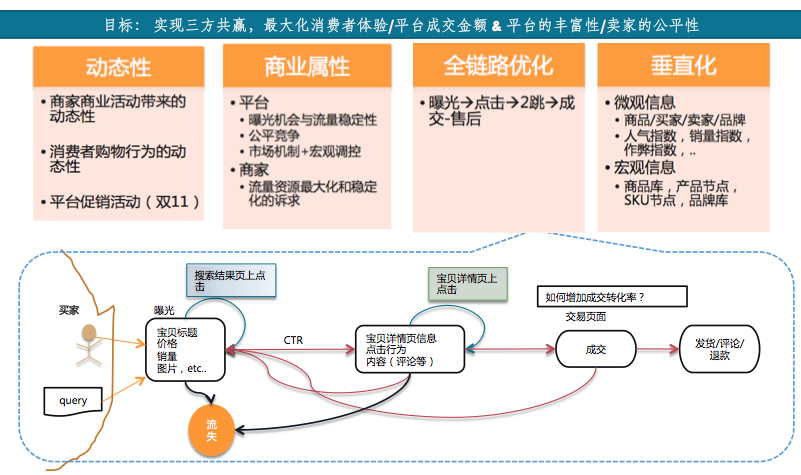
\includegraphics[totalheight=3.0in]{fig/searchProdFea.png}
\caption{电商搜索特性} \label{fig:gansamples}
\end{figure}

淘宝的搜索平台是致力于提供一个一个买家和卖家的公平交易平台;作为一个公平的市场调节员,调整供需平衡,为卖家引导潜在的兴趣用户,以提升其ROI(return on investment),为用户提供满足其需求(user intent)的商品;商业流量下的搜索自然带有其特有的技术特点:

\subsection{动态性}

网页搜索的对象的是分布于各类网站发布的网页,从索引单元上对比,数量上是绝对要远远大于商品搜索的对象集合,如果把每个商品展示页当成是淘宝网站的普通网页的化,表象上讲,商品页面的信息集合应该是网页搜索对象集合的一个子集;网页搜索中的基本对象也存在网页更新,然而淘宝搜索的商品库具有更强的动态性,宝贝的循环搁置,新卖家加入,卖家新商品的推出,价格的调整,标题的更新,旧商品的下架,换季商品的促销,上下架,降价,宝贝图片的更新,销量的变化,卖家等级的提升,商品竞争程度的提升等,都需要淘宝的商品搜索引擎在第一时间捕捉到变化,并及时反映到索引结构中的相应信息单元,而最终的排序环节,这些变化也会动态的融入排序因子,带来排序的动态调整;因此对于商品搜索引擎,要求建立高效的索引更新体系,适应商品类目体系,倒排索引结构,匹配机制的召回逻辑,以及应对商品排序信息及时生效的cache分层机制;

\subsection{全链路优化}

众所周知,相比类似百度这样的网页搜索平台,一个明显的差异是,淘宝搜索平台拥有网购消费者从查询到完成目标商品订单,这样一条完整的行为数据闭合式链路;因此对于用户的一次查询的满意度衡量绝不能止于搜索结果页上看到一个标题相关的商品而发生了点击来判别,post-click之后的商品详情页上的行为,甚至于进入post-pay之后的评论信息都应该成为度量某商品对于某次查询(query)的满意度影响因子;因此,全链路的行为建模会是淘宝搜索体系相比于网页搜索的重要差异之处;既然谈到这点了,再多啰嗦两句,京东也是一家做电子商务的公司,也有着不小的规模,那么如何来看淘宝搜索与京东搜索在全链路优化上的差异呢?从京东模式来看,post-pay环节,由于销售,物流仓储的自营性,可以认为是无差异竞争的;而对于淘宝来说,售后的服务,发货速度,以及纠纷退款等环节是取决于商家与消费者之间的互动来决定的,差异性不言而喻,因此淘宝搜索有必要建立post-pay环节的排序度量因子;

\subsection{商业属性}

电子商务平台的搜索自然具备商业流量的根本属性,商家希望所经营商品通过得到足够的曝光而带来成交;因此,流量资源(曝光)也就成了商家必争之地。搜索排序体系的白盒化和可解释性自然是至关重要。淘宝搜索的ranking,更接近于一个带约束的优化问题,而不是一个简单的排序,优化的目标是最大化平台的成交金额;而约束则是卖家流量分配的诉求;这个环节的涉及到的课题也是电商平台最复杂之处,我会在下面集中阐述下我的一些观点;

\subsection{垂直化}
电子商务搜索属于 vertical search 范畴,相比于网页搜索,对于平台上内容的结构化梳理,以及商业平台上积累的买家,卖家和商品关系数据的挖掘都有更高的要求;因此需要建立 micro analysis 和 macro analysis 双位一体的搜索内容加工体系,宏观分析层面指的是:除了目前已经积累并广泛运用的5级类目之外,完善的商品库建设,spu节点,sku节点,品牌库等,都是必不可少的;微观分析层面则从商品的人气指数,销量指数,作弊指数等角度给出商品自身质量的度量信息;使得搜索结果能够为消费者提供,不仅仅停留在标题相关层面的服务,可以通过合理的宏观分析带来的数据结构化,实现高效的结果查询,通过细致的微观分析,保证优质的商品优先展示给消费者;


\begin{figure}[h]
\centering
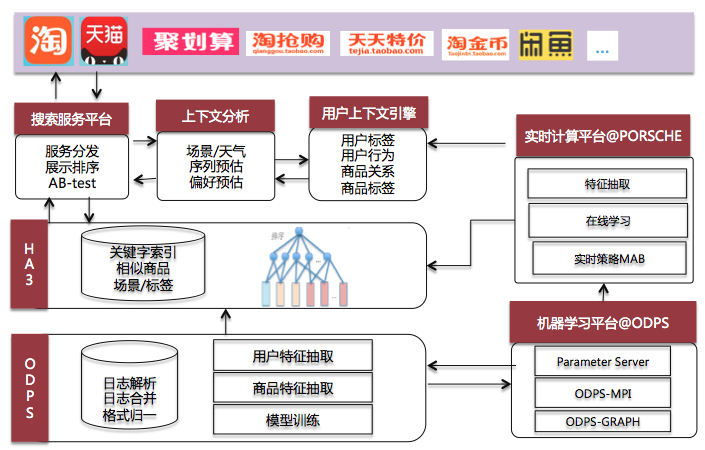
\includegraphics[totalheight=3.0in]{fig/techForBusiness.png}
\caption{智能化助力商业产品} \label{fig:gansamples}
\end{figure}

\section{技术挑战@业务问题} 
\subsection{算法模型} 
像众多互联网企业一样,大数据环境下,基于用户行为建模所面临的技术挑战很多,大家耳熟能详的点列举如下: 
\begin{description}
	\item 投放逻辑带来的数据bias对行为建模的影响
	\item 用户行为数据的稀疏性
	\item 因果关系的模糊性
	\item 用户行为的时效
	\item 行为个性化和非个性化 unified ranking
	\item Cold start modeling
	\item 多样性与精确性的tradeoff (过度个性化)
	\item 长短期个性化融合
\end{description}

\subsection{工程技术} 
随着数据规模的指数级增长,完成复杂数据建模对于工程技术体系的挑战也是不言而喻: 
\begin{description}
	\item 千亿行为和关系数据存储、实时更新和查询
	\item 翻页陷阱
	\item Cache机制
	\item 分级实时体系(数天/小时/秒/ms)
\end{description}

\subsection{效果评估}
效果评估是保证体系迭代朝正向发展的关键保障。
\begin{description}
	\item 模型正确性评估
	\item Ab体系下分群评估
	\item 社会化评测
\end{description} 

\begin{thebibliography}{99}
\addcontentsline{toc}{chapter}{\protect\numberline{}{\hspace{-1.5em}参考文献}}
\markboth{参考文献}{参考文献}
\bibitem{1} C. Burges, T. Shaked, etc.., Learning to rank 
using gradient descent. In Proceedings of the 22nd international 
conference on machine learning, ACM
\end{thebibliography}

 
      %第二章  业务挑战

\chapter{搜索工程和算法架构体系} 
\thispagestyle{empty}

\setlength{\fboxrule}{0pt}\setlength{\fboxsep}{0cm}
\noindent\shadowbox{
\begin{tcolorbox}[arc=0mm,colback=lightblue,colframe=darkblue,title=学习目标与要求]
%\kai\textcolor{darkblue}{1.~~.} \\ 

\end{tcolorbox}}
\setlength{\fboxrule}{1pt}\setlength{\fboxsep}{4pt} 

\section{工程架构} 

\section{算法架构} 

\section{工作流和数据流} 


\begin{thebibliography}{99}
\addcontentsline{toc}{chapter}{\protect\numberline{}{\hspace{-1.5em}参考文献}}
\markboth{参考文献}{参考文献}
\bibitem{1} C. Burges, T. Shaked, etc.., Learning to rank 
using gradient descent. In Proceedings of the 22nd international 
conference on machine learning, ACM
\end{thebibliography}

 
       %第二章  工程算法架构

\chapter{搜索词相关性的技术}
\thispagestyle{empty}

\setlength{\fboxrule}{0pt}\setlength{\fboxsep}{0cm}
\noindent\shadowbox{
\begin{tcolorbox}[arc=0mm,colback=lightblue,colframe=darkblue,title=学习目标与要求]
%\kai\textcolor{darkblue}{1.~~强化学习.} \\ 

\end{tcolorbox}}
\setlength{\fboxrule}{1pt}\setlength{\fboxsep}{4pt} 

淘宝的平台上有数十亿的商品,消费者在平台上想要快速找到自己想买的商品,只能在淘宝搜索输入查询词,也就是我们通常说的query,来表达购物的需求。如果能够理解用户Query背后的购物意图,就能够帮助搜索引擎自动将符合用户意图的商品返回给用户,提升结果的准确率,从而提高用户在平台上的购物满意度和体验。



\section{类目预测}
\subsection{Query类目预测与分析}
用户搜索意图的理解在搜索排序体系下有着重要的作用。要理解用户的意图,一部分可以通过用户的关键词文本来理解语义上的意图;另一方面可以通过用户的行为积累来获得用户的潜在需求意图,即基于用户行为的意图预测
。
\par 文本意图中的类目意图预测是淘宝搜索相关性中的重要组成部分。商品在关键词索引召回之后,在第一轮海选粗排阶段通过类目相关性,可以优先选择更相关类目的商品进入第二轮精排中。一方面保证排序的效率,使得排序在类目相关的商品集合上进行;另一方面从最上层保证类目的相关性,保证用户的体验效果。
\par Query类目预测主要目标是,分析用户的搜索Query和哪些类目的意图更相关。Query类目预测不同于商品类目预测和一般的文本分类问题,主要是因为Query带有的描述信息比较少,而且往往意图比较分散,也就是对于一个用户搜索的Query会有多个可能相关的类目,对预测意图的难度会比较大。例如上图用户搜索“电脑显示器”,其中转接线就属于与用户意图不相关的类目商品。 
\begin{figure}[!h]
	\centering
	\includegraphics[width=0.9\linewidth]{"fig/lm0.png"}
	\caption{}
	\label{fig:lm0}
\end{figure}

\subsection{线上模型实现}
目前线上的版本模型主要包括点击模型和先验模型两部分。
\subsubsection{点击模型}
用户对于搜索的query的点击商品行为,很大程度上反应出类目的相关,即点击越多的类目,越有可能和query的意图在类目维度更相关。
\par 所以点击模型主要依赖于搜索词的历史行为,也就是Query在各个召回商品的类目下的历史一段时间的点击行为做了统计,并且根据各个类目的点击分配比例,通过分数阈值的规则划分类目相关与否的档位。 
\subsubsection{先验模型(新)}
先验模型主要为了解决点击模型带来的马太效应问题,相似类目的点击行为差异和新发类目的商品冷启动问题。
\par 目前依赖的方法主要是是通过Query在类目下的召回结果数以及在类目下商品的占比等因素,相当于商品体量的一个估计。两个模型之后进行融合,通过规则的方式确定相关和不相关的档位阈值。
\subsubsection{在线实现}
每天通过搜索日志中选择一段时间内的中高频Query,通过上述统计规则方法得到Query的类目预测结果,并存储为离线词典。(在线访问时,主要依赖于这份基础数据词典。对于不在词典中的偏长尾的Query,则通过线上丢词的长尾类目预测逻辑进行识别,将在另一篇文章中介绍~)
\subsection{存在的问题与分析}
基于这种融合模型的方法,点击模型带来更准确的类目相关度量,而先验模型对于行为稀疏的类目可以得到召回上的提升,使得线上的相关性效果得到一定的保障。但是在应用中还是存在着以下几个问题:
\par 首先是点击模型,统计历史的类目点击数据对于曝光较多的类目会占优势,对于类目商品体量不均的情况,会使得点击分数更偏向体量大的类目;而且如果存在类目新发商品或新增类目的情况,即使点击数据在近日内有增量,但是也很难在统计值上追上已有类目,所以需要一个根据增量预估整体的方法。其次,在先验模型中的一个重要假设,就是召回的商品越多,越可能是相关的类目,其实并没有考虑语义上是否能保证相关,例如:“茶几”这个Query可以召回“纸巾盒”类目的很多商品,但其实文本语义上这两个意图并不相关。所以先验模型中对于召回的类目,要做语义上的判断和区分。最后,通过人工经验的规则方式将两者融合,得到最终的类目判别结果。而随着商品分布的和用户行为的变化,固定的阈值方法难以满足线上的准确率要求,需要有更合理的综合特征的方式。
\par 基于以上的问题,我们提出了基于DNN+GBDT的类目预测融合模型,对其中的问题进行优化,并得到了准确率的效果提升。在第二部分中会详细介绍每个部分。
\subsection{基于GBDT融合模型的类目预测}
\subsection{基于反馈的模型}
\subsubsection{点击模型(新)}
类似于排序中ctr预估的方法,通过Query和类目下的商品的历史点击行为,预测Query和类目的未来的点击行为。主要使用Query历史7天、15天的曝光、点击等统计特征。
\par 考虑到前面提到的第二个问题曝光带来的不公平点击差异,所以在回归的目标上加上了该类目下展现pv的正则项,使得本身展现高的类目会在未来的展现比例得到一定的弱化。
\subsubsection{价格\&成交模型	}
类目之间的商品的价格差异,在区分类目意图的差异上有着重要作用。
\par 例如,用户搜索“手机”,自然召回的商品有主件“手机”类目和配件“手机保护套”类目,我们可以通过query下的成交价以及各个类目的商品价格加入到特征中。
\par 所以我们建立了一个基于成交和价格的回归模型,同样利用历史的统计信息作为特征主要包括
 
\begin{itemize}
\item query在类目下的成交价格
\item 类目下商品的价格
\item 类目的成交金额
\item query的成交均价等
\end{itemize}
其中的类目下商品价格,为了排除掉过高过低的商品价格,我们在模型中使用在一段时间窗口内,该类目下成交商品价格平均值。
\subsubsection{基于DNN的先验模型(Deep Prior Model)}
首先,对于Query能召回商品的类目的集合可以作为相关类目的一个较小候选集合;然后,对于这部分类目,需要计算词构成的语义的匹配程度的分数。在计算语义的匹配模型中,我们采用了多层神经网络的方法,通过词的embedding方式表示Query和类目,然后通过Query和类目的采样做目标,来训练这个网络。网络结构图如下:
\begin{figure}[!h]
	\centering
	\includegraphics[width=0.9\linewidth]{"fig/lm1.png"}
	\caption{}
	\label{fig:lm1}
\end{figure}

\subsubsection{特征说明}
\begin{itemize}
\item Query Embedding:用每个词id的embedding做组合,其中加入了每个词的统计权重和意图权重。词的统计权重主要为词在Query日志中的搜索pv;意图权重主要为词的标签信息设置的人工权重,例如品牌词、品类词、型号词可能在意图中有更高的权重。最终词的权重表示为 $log( pv ) * tag\_weight $。
\item Category Words Embedding:每个类目下的词,计算tf*idf,这里的idf计算将每个类目作为一个doc,即在越多类目中出现的词,约不重要。选取每个类目下的最高权重的词来表示类目,并进行带权的embedding计算(全连接)。
\item Cate Id Embedding:类目id直接做embedding
\item Cate State Feature:主要为类目下商品的平均成交价等连续值统计特征。
\end{itemize}
\subsubsection{样本\&采样}
样本为Query和类目的pair对,主要来源于以下几个部分:
\begin{itemize}
\item 当前类目与该类目路径名称(其中的词作为Query)为正样本;当前类目和与该类目具有相同父类目(只向上一层)的叶子类目的名称为负样本。
\item 对于有行为的类目,每个类目下随机抽取有行为商品,对每个商品,获取其ctr高的Query作为正样本;同时,这部分Query可以召回的非该行业或一级类目的商品类目为负样本。
\item 对于没有行为的类目和商品,对商品标题中的词做随机采样,作为正样本。此时选择组成Query的词数目有限制,选择过短的随机Query会带来很大的歧义。同时和前面的方法相同,生成的Query召回的非该行业或一级类目的商品类目为负样本。
\item 基于少量人工规则的采样,基于类目之间的互斥关系,Query的正样本类目对应的互斥类目为负样本。
\end{itemize}
\subsubsection{总结\&思考}
\begin{itemize}
\item 为什么使用点击的数据?
\par 点击的样本在准确性上有较高的保证,而且从数据的观察发现,每个类目下的高点击的Query并不一定是和类目相关,但是Ctr高的query往往与类目的关联性很大。而且由于我们丰富了类目的表示,即类目用词来表示的同时也增加了一定的泛化性,也就是说对于词表达比较相似的类目,即使自身行为并不丰富,也可以通过与其表达相似的类目来学习得到和Query的关联性。
\par 选择类目下各个商品的Query与选择类目整体的Query,前者可以带来更丰富的特征,后者可以在统计的丰富上保证准确性。
\item 为什么不使用多分类目标的模型?
\par 最开始设计方案时其实调研过多分类的方案,最后还是选择二分类的框架主要原因有两个:首先 Query的类目预测不同于商品,往往会存在多个合适的类目预测结果,所以如果采用Softmax loss的多分类,则会由于loss本身的限制,难以使得多个类目同时为正,就算是整体的平均loss最低,对于多label的样本中的loss也是比较高;另外,最重要的一点是先验模型的计算是可以预先知道候选类目的,也就是通过召回限制,可以得到Query的候选类目在一个小的集合范围中,相比多分类的全label空间,要缩小了很多倍(15000->50),而且如果以类目作为特征而不是label,可以得到很多类目的统计以及描述类特征。
\end{itemize}
\subsection{基于GBDT的Ensemble模型}
前面所述分别从行为反馈和商品分布得到不同维度的相关性描述,在线上版本的模型中对于各个特征采用分数的规则来决策得到最终的相关类目。我们改进了原有通过人工经验的方式设置相关性分档的规则,通过人工标注的样本,将多个特征通过GBDT模型做最后的决策分档模型。整体图如下:
\begin{figure}[!h]
	\centering
	\includegraphics[width=0.9\linewidth]{"fig/lm3.png"}
	\caption{}
	\label{fig:lm3}
\end{figure}
目前在GBDT的特征包括:
\begin{itemize}
\item 先验模型分数(Deep Prior Score)
\item 点击分数、价格\&成交分数,在Query下所有类目的归一化、比例等。
\item Query召回类目下的商品数、占Query的商品数比例、占类目下的总商品比例。
\item Query分词长度、Query召回的类目总数(描述宽泛性的Query)
\item 类目所属的一级类目、行业等
\end{itemize}
\subsection{模型效果与分析}

\subsubsection{数据效果 \& 页面效果}	
新老版本效果对比,Query搜索“电脑显示器”,类目预测的结果对比(上图为老版本,下图为新版本)
\begin{figure}[!h]
	\centering
	\includegraphics[width=0.9\linewidth]{"fig/lm4.png"}
	\caption{}
	\label{fig:lm4}
\end{figure}

\begin{figure}[!h]
	\centering
	\includegraphics[width=0.9\linewidth]{"fig/lm5.png"}
	\caption{}
	\label{fig:lm5}
\end{figure}
在页面BTS的商品类目对比效果:
\begin{figure}[!h]
	\centering
	\includegraphics[width=0.9\linewidth]{"fig/lm6.png"}
	\caption{}
	\label{fig:lm6}
\end{figure}

\subsection{指标效果}
先验模型的训练中用人工标注的样本作为validation集合,通过网络参数以及样本的分布调整,模型在验证集合的auc可以达到0.8。
\par 人工评测整体模型时会根据算法产生的类目档位相关(2档)、不相关(1档)进行准确率和召回率的判别,主要关注的是2档类目的准确率和召回率。样本抽取时为了更好的暴露各个行业中可能存在的问题,采用分别对每个行业下按照Query pv分布进行采样的方法。在评测样本中,新方法相比老的方法在2档准确率上有10\%左右的提升(68.51\%->78.75\%),召回率略有下降1.61\%(60.98\%->59.37\%)。(因为评测采样的数据样本是每个行业的覆盖量在同样的量级,所以对于较难的长尾行业的数据也会放大,相比线上真实的流量比例,是偏难的一种评测方法)。目前整体的模型数据已经在主搜PC开始BTS。
\par 从效果看对于覆盖率的提升空间还比较大,主要源于一些宽泛Query例如搜索品牌、宽泛描述的品类等问题,对于子品类类目的覆盖率需要在先验模型的采样优化中多加考虑;而且在一些长尾行业的类目上的预测准确率还是需要提升,因为行为比较稀疏,需要更多的商品分布特征。
\par 后续的优化空间主要在先验模型的部分和整体模型的调优,现在只有基于DNN的网络,后续可以考虑更有局部特征能力的CNN和全局性表示的LSTM作为Query和类目的表示。目前由于受限于人工标注样本的数量限制,没有办法做到end to end的整体框架模型,这个也是后续值得优化的一个方向。


\section{基于类目树结构的query长尾类目预测}
\subsection{背景介绍}
\subsubsection{淘宝的类目树体系介绍}
淘宝上有上亿的商品,通过类目来管理这些商品。类目就是商品分类,是商品信息的一种结构化描述,目的是为了管理、导购。淘宝的类目是树状结构的,如下图。一个类目可以细分为更多的下一级类目。类目id=0的类目叫根类目;没有下一级类目的类目叫叶子类目;没有上一级类目的叫一级类目(实际上,一级类目的父类目是根类目,但是根类目是大家不可见的虚拟类目,因为可以认为没有);有下一级类目的类目是下一级类目的父类目;有上一级类目的类目是上一级类目的子类目。如图为例:“电烤箱”、“电饭煲”、“电压力锅”、 “电蒸锅”、“微波炉”等就是叶子类目;“厨房电器”就是一级类目;“厨房电器”是“电烤箱”、“电锅煲类”、“微波炉”的父类目;“电烤箱”是厨房电器的子类目;大家也常常叫一级类目的子类目为二级类目,二级类目的子类目为三级类目,依次类推。淘宝类目树体系的数据一般可以通过tbcdm.dim\_tb\_cate表获取。
\begin{figure}[!h]
	\centering
	\includegraphics[width=0.9\linewidth]{"fig/cwlm0.png"}
	\caption{}
	\label{fig:cwlm0}
\end{figure}
\subsubsection{基于类目树的类目预测}
query的类目预测是淘宝搜索相关性的重要组成部分,通过类目预测,可以把与用户搜索query意图相关的类目对应的商品靠前呈现,从而保证用户的体验效果。
\par 对于高频的query,淘宝已经积累了用户的一些行为数据和统计信息,通过这些数据[建立模型](https://www.atatech.org/articles/85571)往往可以取得较好的预测效果。但对于低频的query,由于缺乏足够的反馈数据,只能通过query本身的语义来推测query意图相关的类目,本文将低频query的类目预测定义为长尾类目预测。
\par 长尾类目预测问题,是一种[multi-label的分类问题](http://ieeexplore.ieee.org/document/6471714/),可以考虑转为multiclass的方式来处理。之所以将multilabel问题转为multiclass问题是基于如下考虑:
\begin{itemize}
\item multilabel的标注数据比较难获取,对于一个query,要罗列出它所有相关的类目很困难,现有top query的2档类目预测准确率也才80\%;
\item multilabel大多数模型是把二档类目都当做同样重要的label来处理,但由于行业下商品、用户行为差异,一个query对应的2档类目分布应该有主次之分,例如"连衣裙"在"女装-->连衣裙"类目应该占大多数,在"大码女装"类目下应该占少数。
\end{itemize}
传统处理多分类的方式利用softmax得到每个节点的概率,对应淘宝的类目预测即只预测**叶子类目**出现的概率,这种方法存在着三个严重的缺陷:
\begin{itemize}
\item 淘宝叶子类目存在着上万个,直接预测上万个叶子类目对应的概率,一方面每次需要对上万个节点计算对应的值,复杂度较高,另一方面softmax函数在top 1的概率区分度较好,但top3-5的类目往往概率值都很接近
\item 没有利用淘宝类目树的体系,相当于只取了类目树叶子节点的信息进行分类
\item softmax划分两档类目难以确定阈值,top K的处理方式对处理宽泛query或明确意图query都不准确
\end{itemize}
为了合理利用淘宝类目树的信息,我们提出了基于类目树的层次分类(以下简称层次分类)方法,其效果如下图,对于query"实木欧式床",我们先预测其到一级类目"住宅家具"、"家装主材"、“尿片/洗护/喂哺/推车床"的概率,然后逐层传导,得到对应每个叶子节点的概率。"实木床”的概率为0.8260是按如下公式计算的,即将概率值逐层传导:
$$P(实木床|实木欧式床) = P(实木欧式床|实木欧式床)\times P(床类|住宅家具,实木欧式床)\times P(实木床|床类,实木欧式床)$$
\begin{figure}[!h]
	\centering
	\includegraphics[width=0.3\linewidth]{"fig/cwlm1.png"}
	\caption{}
	\label{fig:cwlm1}
\end{figure}
基于类目树的层次分类方法相比softmax有着明显的优点:
\begin{itemize}
\item 层次分类可以直接得到各个父节点的概率
\item 层次分类做预测时计算量会小很多,可以考虑树分层遍历贪婪地选出出现可能性大的类目,例如在预测一级类目时直接把概率值较低的类目的分支就不进行预测了。如果贪婪的方式选取每个父节点top的子节点进行预测,层次分类只需要对至多$3^{6}=729$个叶子节点排序取topK, 而softmax则需要对1万多个节点排序取topK
\item 层次分类的准确率会优于softmax分类,层次分类每次对几十个类目预测相应概率,而层次分类是一次对一万多个类目预测概率。实验的效果也证明层次分类预测到叶子类目的准确率比softmax高5\%。
\end{itemize}
本文接下来几章将重点介绍层次分类,具体如下:
\begin{itemize}
\item[-] 第二章主要介绍下业界常用的层次分类模型
\item[-] 第三章主要介绍基于类目树的层次分类的模型及公式推导
\item[-] 第四章主要介绍淘宝长尾类目预测模型的整体框架及相关实验总结
\end{itemize}
\subsection{相关研究}
大规模层次分类领域,业界有很多研究,主要的研究方向在文本分类、蛋白质结构识别等领域。在[A Survey of Hierarchical Classification Across Different Application Domains](https://link.springer.com/article/10.1007/s10618-010-0175-9) 中介绍了常用的层次分类方法, 
\par 主要有三大类:
\begin{enumerate}
\item 平面分类
\item 局部分类器
\item 全局分类器
\end{enumerate}

\subsection{平面分类(Flat classification)}
如下图示例,不考虑类别层次,将类别树种所有叶子节点看做相互独立的平级类别,作为一个多类别分类问题(multi-class)处理,一般使用softmax函数预测各个叶子的概率,选top K作为预测结果。常见的文本分类、手写数据识别都是使用softmax做分类。
\begin{figure}[!h]
	\centering
	\includegraphics[width=0.3\linewidth]{"fig/cwlm2.png"}
	\caption{}
	\label{fig:cwlm2}
\end{figure}

\subsection{局部分类器(Local-model hierarchical classification approaches)}
局部的分类器的方法又细分三类
\begin{enumerate}
\item 预测每个节点
\item 每个母节点建立分类器
\item 逐层分类
\end{enumerate}

\subsubsection{预测每个节点(Local classifier per node approach)}
如下图,对每个节点(叶子和非叶子)建立二分类模型预测,得到所有预测为1的节点,然后遍历树结构找到从根节点到叶子节点全为1的路径,这些路径对应的叶子节点就作为输出的label。如果层次结构中有很多节点,这种方法训练的分类器将非常多,正负样本的采集工作量也是巨大的。
\begin{figure}[!h]
	\centering
	\includegraphics[width=0.3\linewidth]{"fig/cwlm3.png"}
	\caption{}
	\label{fig:cwlm3}
\end{figure}

\subsubsection{每个母节点建立分类器(Local classifier per parent node approach)}
如下图,基本想法就是给每个非叶子节点建立分类器,想法比较直观,本文的层次分类模型主要借鉴该方法。该方法的缺点是无法用在有向无环图的结构里。
\begin{figure}[!h]
	\centering
	\includegraphics[width=0.3\linewidth]{"fig/cwlm4.png"}
	\caption{}
	\label{fig:cwlm4}
\end{figure}

\subsubsection{逐层分类(Local classification per level approach)}
如下图,逐层建立分类器进行。这种方法在近几年的论文中结合神经网络使用较多,如[Hierarchical Classification of Gene Ontology-based Protein Functions with Neural Networks](http://pdfs.semanticscholar.org/0a0c/8c6eab6152910da4165688b2352cc8261d19.pdf)就是使用这种方法改进的网络, 第一层的预测结果作为特征加入第二层中训练,每层的激活函数都是logistic,通过卡一个阈值来输出multi-label。
\begin{figure}[!h]
	\centering
	\includegraphics[width=0.3\linewidth]{"fig/cwlm5.png"}
	\caption{}
	\label{fig:cwlm5}
\end{figure}

\begin{figure}[!h]
	\centering
	\includegraphics[width=0.3\linewidth]{"fig/cwlm6.png"}
	\caption{Hierarchical Classification of Gene Ontology-based Protein Functions with Neural Networks}
	\label{fig:cwlm6}
\end{figure}


\subsubsection{全局分类(Global or big-bang classifier)}

根据整个类别层次学习一个分类模型。如[Decision Trees for Hierarchical Multi-label Classification](https://link.springer.com/article/10.1007/s10994-008-5077-3)就通过决策树来学习一个全局模型。Cai等人基于SVM构造层次分类方法,利用类别层次信息构造判别函数,由SVM模型计算文档在某个类别以及该类别所有祖先类别上得分,然后将这些得分加权作为文档最终得分,以此判别文档类别。
\begin{figure}[!h]
	\centering
	\includegraphics[width=0.3\linewidth]{"fig/cwlm7.png"}
	\caption{}
	\label{fig:cwlm7}
\end{figure}

\subsection{本文层次分类模型介绍}
本文层次分类层的实现方法类似于word2vec中hierarchical softmax的方法,计算从根节点到叶子节点这条路径的概率,路径的概率是按每个非叶子节点走到其子节点概率之积,即损失函数是取**负对数似然函数**。
\par 层次分类模型中主要用到了树结构的概率逐层传导,我们通过对每一层建立判别模型可以简化层次分类的计算。假设query输入数据传入的为K维的向量X,对某一父节点$C_{父}$,其子节点为$C_{子i}, i \in \{1,2,\dots,M\}$,则应该满足概率$\sum\limits_{i}P(C_{子i}|C_{父},X)=1$。从$C_{父}$到$C_{子i}$计算概率是一个明显的多分类问题,我们可以用softmax函数做分类来处理,只是这里的M比较小,一般是2-20。

\subsubsection{基本定义}
为了方便说明,我们定义一些符号,
\begin{enumerate}
\item query输入为K维的向量X
\item 设某条选中的类目全路径(从根节点到叶子节点)长度为$l_{c}$.
\item 设对应的类目树全路径节点为$c_{0}、c_{1}、\dots、c_{l_{c}}$, 其中$c_{0}$为根节点,$c_{1}$为行业,$c_{l_{c}}$为叶子节点,一般$l_{c}$不大于7.
\item 每个$c_{i}$对应的子节点数定义为$N_{c_{i}}$, 其中$i \in \{0,1,2,\dots,l_{c}-1\}$
\item 每个$c_{k}$对应在父节点的位置为$I_{c_{k}}$, 其中$k \in \{1,2,\dots,l_{c}\}$, 且有$0\leq I_{c_{k}} \leq N_{c_{k-1}}-1$
\item 每个非叶子节点对应的向量为$\theta_{c_i}\in R^{N_{c_{i}}\times K}$, 其中$i \in \{0,1,2,\dots,l_{c}-1\}$, $\theta_{c_{i}}^{(t)}$表示$\theta_{c_{i}}$第t行的向量
\end{enumerate}
\par 针对i=$1、2、\dots、c_{l_{c}}$, 我们用softmax得到每个节点$c_{i}$的条件概率,公式如下(假设b相同):

\begin{align}
P(c_{i}|X,c_{i-1}) = \frac{\exp(\theta_{c_{i-1}}^{(I_{c_{i}})}\times X)} {\sum_{s=0}^{N_{c_{i-1}}-1} \exp(\theta_{c_{i-1}}^{(s)} \times X)}
\end{align}

\subsection{损失函数定义}
层次分类的损失函数类似word2vec,用**负对数似然函数**。我们把multi-label输入的样本转为multiclass的样本作为训练,即每次传入的数据是(query,cate)这样的单样本,对每个样本而言,其损失函数的计算公式如下:
$$L=\sum_{i=1}^{l_{c}}L(c_{i})=-\sum_{i=1}^{l_{c}} \ln P(c_{i}|X,c_{i-1})=-\sum_{i=1}^{l_{c}}\ln\frac{\exp(\theta_{c_{i-1}}^{(I_{c_{i}})}\times X)} {\sum_{s=0}^{N_{c_{i-1}}-1} \exp(\theta_{c_{i-1}}^{(s)} \times X)}$$

$$L_(c_{i}) = \ln (\sum_{s=0}^{N_{c_{i-1}}-1}\exp(\theta_{c_{i-1}}^{(s)} \times X))- \theta_{c_{i-1}}^{(I_{c_{i}})}\times X$$

\subsubsection{前向传播计算}
前向传播主要是计算top的Loss值,可以根据Loss的公式由全路径节点为$c_{0}、c_{1}、\dots、c_{l_{c}}$计算得到
\subsubsection{反向传播计算}
反向传播类似于[word2vec](http://blog.csdn.net/itplus/article/details/37969979)  中推导的方式,求出对$\theta、X$的偏导。
\par 以下偏导的计算公式是对单个训练样本而言的,如果是batch训练,则通过循环对每个样本更新反向传播值。
\subsubsection{非路径上的$\theta$偏导}
非类目全路径上的偏导为0
\subsubsection{关于路径上$\theta$偏导}
对于每个$\theta_{c_{i}}^{(t)}$而言(其中$i \in \{0,\dots,l_{c}-1\}$),关于L的偏导只和$L(c_{i+1})$有关,故偏导K维向量如下:
\begin{itemize}
\item[-] 当 $t\neq I_{c_{i+1}}$时偏导为
$$\frac{\partial L(c_{i+1})} {\partial \theta_{c_{i}}^{(t)}} = \frac{\exp(\theta_{c_{i}}^{(t)}\times X)}{\sum_{s=0}^{N_{c_{i}}-1} \exp(\theta_{c_{i}}^{(s)}\times X)}$$
\item[-] 当$t= I_{c_{i+1}}$时偏导为
$$\frac{\partial L(c_{i+1})}{\partial \theta_{c_{i}}^{(t)}}=\dfrac{\exp(\theta_{c_{i}}^{(t)}\times X)}
{\sum_{s=0}^{N_{c_{i}}-1}\exp(\theta_{c_{i}}^{(s)}\times X)}-X$$
\end{itemize}
\subsubsection{关于路径上X偏导}
可以先求关于每个$L(c_{i})$的偏导
$$\frac{\partial L(c_{i}) }{\partial X} =\sum_{s=0}^{N_{c_{i-1}}-1} \dfrac{\exp(\theta_{c_{i-1}}^{(s)}\times X)}{\sum_{s=0}^{N_{c_{i-1}}-1}\exp(\theta^{(s)}_{c_{i-1}}\times X)} \times \theta^{(s)}_{c_{i-1}}-\theta_{c^{i}}^{(I_{c_{i}})}$$

$$\frac{\partial L}{\partial X} = \sum_{i=1}^{l_{c}} \frac{\partial L(c_{i}) }{\partial X}$$


\subsection{层次分类基本框架}

前面介绍了层次分类的的损失函数、前向、后向传播的定义,下面我们具体看下层次分类层的实现框架,如下图:
\begin{itemize}
\item[-] Hierarchical loss layer(图的左边部分), 主要用于层次分类的模型训练
\begin{itemize}
\item[*] 输入K维向量X,及其label为叶子类目cate\_id,以及淘宝类目树结构
\item[*] 前向传播计算损失函数L,是根据传入的cate\_id得到对应在类目树的路径,然后计算每个节点对应的损失函数$L(c_{i})$,然后对loss求和得到$L=\sum_{i=1}^{l_{c}}L(c_{i})$
\item[*] 反向传播则根据类目全路径,将偏导传给底层,得到$\frac{\partial L}{\partial X}$
\end{itemize}
\item[-] Hierarchial predict layer(图的右边部分), 主要用于层次分类的模型预测。模型利用已训练好的层次分类参数及结构进行预测,使用贪婪的算法处理(例如每个父节点选top3的子节点进行计算),通过树的层次遍历,可以得到概率值较高的叶子类目,以此作为输出。
\end{itemize}

\begin{figure}[!h]
	\centering
	\includegraphics[width=0.3\linewidth]{"fig/cwlm8.png"}
	\caption{}
	\label{fig:cwlm8}
\end{figure}

\subsection{前、后向传播优化}
我们注意到损失函数L可以把沿路径计算loss问题(左图)转化为右图展开形式,并行计算,互相不受影响。

\begin{figure}[!h]
	\centering
	\includegraphics[width=0.3\linewidth]{"fig/cwlm9.png"}
	\caption{}
	\label{fig:cwlm9}
\end{figure}

\subsection{基于层次分类的query类目预测}

我们利用层次分类模型来完成淘宝query的长尾类目预测,模型训练的主要框架如下:
\begin{itemize}
\item[*] 输入数据有三部分:
\begin{itemize}
\item[-] Query,用户输入的query
\item[-] Label, 训练时使用的label数据
\item[-] Tree structure, 淘宝的类目树结构,用于层次分类模型构建和先验概率计算
\end{itemize}
\item[*]  特征提取:
\begin{itemize}
\item[-] 从输入Query提取语义相关的特征(semantic feature),
\item[-]从淘宝用户历史行为、商品历史分布中提取统计特征(statistical feature)
\end{itemize}
\item[*]  通过神经网络组合特征进行学习,然后用层次分类模型做训练和预测
\end{itemize}

\begin{figure}[!h]
	\centering
	\includegraphics[width=0.3\linewidth]{"fig/cwlm10.png"}
	\caption{}
	\label{fig:cwlm10}
\end{figure}

下面分别从数据和模型详细介绍下我们的工作,类目预测划档的工作不在上面框架图中,我们会在本章第三节介绍下相关工作。

\subsection{训练数据}
深度模型通常需要大量训练数据,但对于长尾query而言,multilabel问题中高质量的标注label难以获取。我们考虑一些规则的方法,获取训练数据
\begin{itemize}
\item[*] top Query的的数据。top Query由于存在用户的行为数据,往往类目预测准确率较高,我们可以根据一些规则,提取top Query的训练数据,以此来迁移学习长尾类目预测:
\begin{itemize}
\item[-] 每个商品关联的top K的query
\item[-] 历史top query对应的2档类目
\end{itemize}
\item[*] 商品标题及其对应类目。商品放置的类目是最为准确的label,虽然标题数据与query分布上存在着差异,但可以使用标题的数据预训练,得到词和字符的向量表达
\item[*] 标题词采样。标题词采样生成query由于生成query的质量难以保证,准确率较低。
\item[*] 人工标注积累的一批长尾query及其label。
\end{itemize}

\subsection{特征提取}
query长尾类目预测可以提取的特征主要有两部分组成:
\begin{enumerate}
\item 语义特征。语义特征主要是query本身表达的语义,这可以从词、字符维度通过DNN/CNN/LSTM等方式学习query的语义表达,如上面框架图中分别对query以词、字符维度做了embedding, 然后再分别得到query的语义表达向量(128~256维)。另外语义特征还可以考虑词用word2vec预训练,加入词性、tagging等特征(框架图中未画出)等。
\item 统计特征。统计特征主要是从query或词的历史行为数据来获取特征,主要包括:(a)词在各类目分布,互信息;(b)词在搜索中的pv,uv,gmv,ctr,互信息;(c)query历史的pv,uv,gmv,ctr;(4)相似query历史的pv,uv,gmv,ctr;
\end{enumerate}
上面框架图中的特征提取工作如下:
\begin{itemize}
\item[*] 对query归一化后提取语义特征:
\begin{itemize}
\item[-] 中粒度分词进行embedding操作(50w词表), 每个词128维向量表达,之后通过DNN/CNN等方式得到query的语义向量128维
\item[-] 提取query中的字符进行embedding操作)(7000个字符),每个字符64维向量表达,之后通过DNN/LSTM等方式得到query的语义向量128维
\item[-] 把词维度表达的语义向量和字维度表达的语义向量concat,得到256维语义向量
\end{itemize}
\item[*] query归一化后提取统计特征,这里主要考虑通过词类目分布来预估query的类目分布
\begin{itemize}
\item[-] 根据一定规则得到每个词的先验分布
\item[-] 根据词加权平均得到query的类目先验分布,见下面"苹果手机"例子
\item[-] 得到query在叶子类目的概率分布后,以类目树结构解析得到每个节点的概率
\item[-] 将叶子节点和非叶子节点铺平,按概率值降序排,截断top 300的节点及其值作为query的先验类目特征
\item[-]将top300的先验类目特征由稀疏值转为1.5万维向量
\end{itemize}
\item[*] 将语义特征和统计特征做全连,得到组合特征。
\end{itemize}

> 若词"苹果"先验类目概率分布如:  新鲜水果>>苹果:0.5 ,手机:0.5
词"手机"先验类目概率分布如: 手机:0.4,手机壳:0.4,手机配件:0.2
则query"苹果手机"对应的类目先验分布为:手机:$0.5\times w1+0.4\times w2$,手机壳:$0.4\times w2$,苹果:$0.5\times w1$,手机配件:$0.2\times w2$

\subsection{规则划档}
query的特征经过层次分类模型后,我们可以得到query在类目树中的概率分布,我们可以贪婪的选出叶子节点概率值最大的top 20个类目作为候选类目,在这些候选类目中进行划档。

\par 现阶段划档使用的是规则划档,主要有两个规则:
\begin{enumerate}
\item 叶子节点概率大于一定阈值(如0.05概率)
\item 类目全路径下子节点在父节点下概率大于一定阈值(如0.15)
\end{enumerate}

如query “衣柜 简约现代 经济型 宜家”,规则可以方便的将"衣柜"、"简易衣柜"划为2档

\begin{figure}[!h]
	\centering
	\includegraphics[width=0.3\linewidth]{"fig/cwlm11.png"}
	\caption{}
	\label{fig:cwlm11}
\end{figure}

在实验中划档也考虑了简单的模型版划档,效果和规则版相当,后期有时间可以优化模型版划档

|分组| 模型 | 准确率| 召回率 | F1| 备注|
| ------| ------ | ------ |------| ------ | ------ |
|baseline|规则版  |0.8194|0.6194|0.7055|规则是子节点在父节点下出现的概率大于0.15,叶子节点概率大于0.05|
|组一|xgboost|0.8151|0.5897|0.6844|xgboost用1w个query数据训练(每个query10条记录),特征是query层次分类各层概率|
|组一|xgboost|0.8061|0.6253|0.7043|xgboost用1w个query数据训练,特征是query层次分类各层概率+各层相对前一层概率+先验各层概率+先验各层相对前一层概率|

\subsection{实验效果及评测}

\begin{figure}[!h]
	\centering
	\includegraphics[width=0.9\linewidth]{"fig/cwlm12.png"}
	\caption{}
	\label{fig:cwlm12}
\end{figure}


\subsubsection{模型实验对比}
|分组|分类模型| 特征选用|准确率 | 召回率| F1|备注|
|------|------ |------ |------ |------ |------ |------ |
|基准|baseline| |0.5736| 0.8634| **0.6893**|线上现有长尾方法, 作为baseline|
|分组一|softmax|word+char的语义特征| 0.6632 | 0.5725 | 0.6145 |只考虑使用word,char得到的语义特征,用了DNN提取特征,最后分类模型是直接用softmax预测1.2w的叶子类目|
|分组一|softmax|word+char的语义特征+统计特征| 0.6804 | 0.5984 | 0.6368 |在上面基础上加了query的类目先验分布统计特征,其他相同|
|分组二|hierarchical|word+char的语义特征|0.7342| 0.5765| **0.6459** |只考虑使用word,char得到的语义特征,用了DNN提取特征,最后分类模型是使用层次分类模型后规则划档|
|分组二|hierarchical|word+char的语义特征+统计特征| 0.7911|0.6582| **0.718**|在上面基础上加了query的类目先验分布统计特征,其他相同|

从上表可以看出,层次分类模型优于直接对叶子类目分类的softmax模型

\subsubsection{人工评测结果}
人工评测整体模型时会根据算法产生的类目档位相关(2档)、不相关(1档)进行准确率和召回率的判别,主要关注的是2档类目的准确率和召回率。下面是评测结果,可以看出层次模型准确率较高,但召回率偏低,主要的原因是宽泛Query往往只给2-3个类目划为2档,如query“耐克魔术贴女鞋nike”,"女童外套春秋2017新款 韩版"。

| 算法 | 评测数据 | 准确率 | 召回率| 2档丰富度|
| ------| ------ | ------ |------ |------ |
| 层次模型 | 按行业比例采样300个长尾query | 77.04\%|51.03\%|1.84|
| 线上长尾算法 | 按行业比例采样300个长尾query| 63.63\%  | 65.59\% | 2.87|
| 层次模型 | 按pv采样300个长尾query | 88.12\%|52.98\%|1.74|
| 线上长尾算法 | 按行pv采样300个长尾query| 63.63\%|60.60\%|2.66|

\subsection{后续计划}
\begin{enumerate}
\item 完善统计特征的生成逻辑。现有的统计特征计算方式最大的问题会带来大量噪声,如"男拖鞋"query,词"男"会带引入大量与拖鞋不相关的类目的统计信息
\item 确保模型的稳定性。现有类目预测模型有一个很大的问题是query加上一些不相关词后类目预测结果变化较大,或者无法预测。后续考虑在模型中通过attention机制确保中心词相关的类目能预测正确。
\item 融入知识型数据到类目预测模型中。例如将上下位宽泛词、同质类目、互斥类目等规则信息融入到模型中。
\item 考虑和querytagging、相关性等模型一起进行multitask的学习
\end{enumerate}



\subsection{导购思考} 
导购产品包含了底纹、搜索发现、首页分类、下拉等产品,主要功能是在搜索前与搜索中为用户提供便利的搜索引导。因此,为用户提供更加便捷的导购路线,以及让更多的用户使用导购产品,对搜索用户的增长有一定的促进作用; 
当用户使用搜索时,他是有一定的明确需求的,而随着推荐类产品的不断发展,如直播、资讯等,老用户的使用习惯也在发生着变化,从之前的用户主动的需求发起,到现在的用户等待信息的供给,随着用户心智的变化,我们在产品上也需要因势利导的做出更满足用户需求的产品。另一方面,随着用户市场的下沉与扩展,在用户增长的前提下,势必会有大量的淘宝新用户进来,这批用户可能对如何使用搜索并不太熟悉,因此在产品方面,我们需要有更加方便易用的产品形态服务用户; 

导购算法经过了多年的发展与优化,目前已经在召回、排序以及调控策略上有了较深的积累,这也促使我们不断思考如何在新形势下做出更满足用户需求的算法,从当前所面临的问题出发,我们主要从以下几个方面进行了思考:

\begin{enumerate}
	\item 多领域联合: 导购产品包含了多个产品形态,而目前这几个产品形态之间是相互割裂的,在样本、特征以及用户反馈上并没有做到信息上的共享与利用,因此如何将这多个领域进行联合起来,作为一个统一的导购整体,并达到1+1>2的效果,是我们面临的一个主要问题

	\item 用户全生命周期表示: 导购产品分别是在用户无输入情况下为他推荐Query,以及在用户有部分输入情况下进行Query补全,因此对用户的全方位的理解也是所面临的一个问题,比如是否新用户、用户的活跃程度,或者是用户即将流失的状态; 另一方面,如何积累用户的长期行为,比如一年前的行为,而目前的sequence学习方法可能会更加强调当前的行为,而遗忘了较长时间前的信息,所以如何基于lifelong learning的学习机制,对用户的长期knowledge进行积累,并进行不断的累加学习,也是我们需要研究的一个课题

	\item 个性化与多样性的权衡: 目前的导购产品中,比较重视用户的个性化,之前也尝试过在个性化与多样性之间进行一些平衡,但对指标在短期内有一定的负向影响。但如果考虑较长的时间范围,多样性对于用户的活跃度是有正相关的,所以如何在个性化与多样性之间进行平衡,同时通过长期收益来评价效果,也是在导购下需要解决的一个问题

	\item 用户意图识别的负反馈: 在Query推荐场景下,对于用户的负反馈也面临较多的挑战,尤其是在伪曝光的前提下。因为在实际中,我们虽然在搜索框的底纹中,给用户推荐了某个Query,但是他到底有没有真正看到,或者说看到了也确实满足他的意图,但因为各种原因,跳到了其它app上,所以这部分样本不能直接作为负样本。如何获取到用户真正不满意的推荐Query,以及通过bandit的方式将其在后续的推荐中进行一定程度的降权,也是我们在持续优化的一个点

	\item 推荐中的组合优化问题: 今年在底纹中做了较大的产品升级,从之前的单个底纹到现在的多个底纹轮流滚动的形式,在算法上就从之前的top1问题转换到了现在的topN问题,如何决定N的值,以及根据用户的浏览宽度等决定不同类目的组合也是一个新问题,比如有的用户的兴趣点比较狭窄,可能这N个Query就偏向于这一个意图,有的用户兴趣比较发散,我们就可能会在类目宽度上放得更广

\end{enumerate}

搜索导购包含了多个产品形态,如底纹、首页分类、搜索发现以及下拉等产品形态,在产品定位上我们有下面的思考: 

\begin{figure}[!h]
	\centering
	\includegraphics[width=0.9\linewidth]{"fig/20210621225243.png"}
	\caption{}
	\label{fig:20210621225243}
\end{figure}

在用户路径上,底纹、首页分类以及搜索发现是在用户发起搜索前的无Query情况下的推荐,更加关注的是对于用户意图的理解与推荐。而在下拉场景下,当用户已经输入了某个前缀词之后,我们会从效率和个性化两个方面,为用户提供更好的下拉服务

\begin{figure}[!h]
	\centering
	\includegraphics[width=0.9\linewidth]{"fig/20210621225404.png"}
	\caption{}
	\label{fig:20210621225243}
\end{figure}

作为一个导购的平台,对于用户的全生命周期学习与表示能够更好地识别用户意图,同时在不同场景下的样本、特征共享,可以将一个domain的信息平滑的迁移到另一个domain中,这两个方面我们在底纹中进行了初步的尝试。召回与排序一直是算法的核心,今年我们在下拉中尝试了文本生成作为召回的扩展,同时在排序上也加入了position bias的机制来解决位置所带来的偏差; 

底纹: 底纹是导购中非常重要的一个产品,当用户打开手淘首页时,底纹推荐词就随之出现。因此底纹词推荐的精准性对于吸引用户进入搜索是至关重要的。底纹词在这里承接了唤起用户搜索记忆以及提供更精准Query的功能。今年我们在底纹方面尝试了多种产品形态的优化以及算法优化。在产品形态上,今年上半年尝试了多底纹同时展示的产品形态,最终采用了当前的多个底纹词滚动展示的形态。在算法方面,我们分别从召回和排序两个方面进行了升级。主要的优化点有:产品层面上的优化,从传统的单个推荐词到当前的多个词轮播的形式;
召回上,进行了扩覆盖、分层召回以及权益类Query的召回等的扩充;
排序上,我们正在尝试实时联合反馈的LTR排序模型,将多个导购领域的样本、特征进行共享,形成跨领域的学习后续,底纹是导购方面非常重要的算法着力点,后续会继续在lifelong learning、multi-domain learning、组合优化等方面进行长期的深入探索; 

底纹优化的演进历史: 
\begin{enumerate}

\item 基础版本,截止今年7月份之前底纹的产品形态还是跟往年一致,用户每次到达首页会触发一次底纹推荐服务请求,算法返回预测出的最有可能被用户点击的top1个query展示给用户;
\item 多底纹版本,主要考虑到部分用户会在首页停留的时间比较长,如果推给用户的query固定是一个的话没有充分利用到用户的停留曝光机会,我们尝试了在搜索框同时展示1~3个query的样式,但同时会受限于搜索框长度,展示的query不能过长,这一版样式AB效果没有太大变化;
\iteem 滚动底纹,顾名思义是指用户在首页停留期间可以看到多个query固定时间间隔轮播展示,是在以上版本总结和思考的基础上一种新的尝试。既能较好利用用户在首页停留期间的曝光机会,相比基础版本query长度又不会受限,此外加入动效后也能一定程度上吸引用户眼球。经过一段时间bts测试,线上AB效果也符合预期,底纹uctr提升5%;
\item 大促样式,主要在双11当天的大促氛围下对底纹做了颜色加黑加粗的效果强化
\end{enumerate}

底纹的召回和排序优化: 底纹的在线召回以个性化为主,主要的召回类型有偏实时的i2q,q2q,以及偏长期的longtime prefer q,个性化覆盖占比90
\%,众所周知个性化推荐效率要远高于非个性化,那么对于有历史行为的用户如何继续提升个性化覆盖占比,以及对于手淘拉新和用户下沉带来的新用户如何拉新到搜索是这我们在召回优化方面的主要出发点; 
\begin{enumerate}

	\item 整体扩召回,旨在扩大有行为的那部分用户的个性化query召回候选集,主要从i2q,q2q的离线扩覆盖,以及在线拉长用户点击/搜索行为周期入手。通过item的短标题生成,title2query候选集合并等手段,我们的i2q覆盖从原来的3000w宝贝扩充到2.1亿,q2q从覆盖1600w source query扩充到1800w。这块带来的在线效果也比较明显,AB测试使用uv+4\%

	\item 分层扩召回,主要是将无少行为的那部分用户按手淘的新人分层(N0~N8)划分,离线计算每个分层用户偏好的query,在线扩充基于群体的个性化召回候选池,这样做的一个好处是对于纯新登用户来说也能有一定的弱个性化推荐结果

	\item 权益类query,结合之前针对三四线下沉新用户的用研报告,新用户更关注切实的优惠信息,我们尝试了联合运营圈品和获取用户实时红包在底纹透出一些带权益tag类的query,比如“家用拖把 9.9元包邮”等

\end{enumerate}

底纹的排序优化: 在针对新老用户的整体/分层扩召回基础上,我们自然而然会想到排序方面是不是也可以做一些针对性的优化,以下从特征和模型两个方面做简要归纳; 特征,1)user泛化特征强化,新增用户手机品牌、30天浏览类目宽度、浏览卖家数、最近1月手淘访问天数、未来7天气温等特征,离线auc提升1.3\%,在线使用uv也有1个点提升;2)将query维度的先验ctr,引导pv/uv等特征按用户分层细分;
模型,1)新老用户模型分层;2)随着产品形态从单底纹到多底纹滚动的演进,离线模型用最新采样方式采到的样本来更新也能获得不错效果;

基于Bandit重排: 重排阶段是介于精排和最后的展示之间对query排序结果的最后一次在线调整,有时候也称为策略层,一般会考虑排序list的上下文和满足一些体验保障的约束条件(比如类目的重复度等)。在这一阶段我们的优化目标既要兼顾推荐query的点击效率和丰富度,又要结合用户实时反馈尽量减少用户不感兴趣query在下一次的曝光机会。下图展示了底纹重排从最初的精排后topN随机->topN轮播->Bandit重排的优化历程以及背后的思考:

\begin{figure}[!h]
	\centering
	\includegraphics[width=0.9\linewidth]{"fig/20210621230926.png"}
	\caption{}
	\label{fig:20210621230926}
\end{figure}

基于实时联合反馈的LTR排序模型: 在开头问题思考部分我们提到对用户而言从首页跳转到搜索的使用过程中搜前->搜中->搜后是一个连贯而不是割裂的过程,在这个过程中用户实际是跟多个query导购产品有着丰富的交互行为,比如搜索前的底纹,搜索中的下拉、主动输入,以及搜索进入srp页后的锦囊/交互式搜索等。如何将这几个导购产品联动起来,更好地在各阶段满足用户的搜索意图是本部分我们研究的主要出发点。下图是用户从首页跳转搜索过程中与底纹、下拉、主动输入的一个交互示例,在这中间用户提交query的方式有多种,比如底纹、下拉推荐曝光的query有的会被点击,有的只曝光没有有效点击,有点击的我们认为是正反馈,只曝光未点击的是负反馈信息,它们都能一定程度上反应用户在当前时刻的偏好信息;

\begin{figure}[!h]
	\centering
	\includegraphics[width=0.9\linewidth]{"fig/20210621231042.png"}
	\caption{}
	\label{fig:20210621231042}
\end{figure}

传统的底纹、下拉排序任务中都是独立分开优化的,在样本、特征以及用户反馈上并没有做到信息的共享和传递。从上面的分析角度出发,我们思考是不是可以用一种基于实时联合反馈的多任务学习模型,在特征信息层实时拿到用户在各query导购产品的正负反馈时序信息,样本层在各task独有的特征基础上共享联合反馈特征,任务层做multi-task learning,具体如下图所示

\begin{figure}[!h]
	\centering
	\includegraphics[width=0.9\linewidth]{"fig/20210621231132.png"}
	\caption{}
	\label{fig:20210621231132}
\end{figure}

模型结构设计: 基于以上设想,我们提出了一种基于实时联合反馈的LTR排序模型,与上不同的是在实验阶段我们对任务层做了一定简化,通过实时多导购交互的正负反馈特征来学习用户向量,task层先只优化底纹的排序模型。该模型的优化目标是预测底纹推荐给用户的query在未来是否会被点击。相比以往的底纹排序模型特点是在特征层通过利用用户在多导购场景的正负反馈信息强化用户表示。具体来讲模型主要有以下几层: 

\begin{enumerate}

	\item user向量表达层,利用系统之前展示给用户但未点击的底纹query,下拉推荐给用户但未点击的query作为负反馈信息,通过底纹/下拉/主动输入提交的query作为正反馈信息。设计一种Filter Attention结构,利用这些负反馈信息来衡量用户以往意图中哪些意图在下一步将会减弱,反之负反馈中的无效曝光也可以一定程度上被鉴别

	\item user向量表达拼接传统的统计特征和候选query特征,因为原有特征也包含了trigger,user,query的丰富信息

	\item 经过多层全连后,学习点击/不点击二分类问题的交叉熵损失函数

\end{enumerate}




下拉: 手淘的下拉推荐是流量最大的导购产品和搜索发起途径,日均使用uv 1.05亿,占搜索uv的75\%以上;通过下拉推荐的引导pv占总的搜索pv 46\%左右,比用户主动发起搜索的比例还要高。同时下拉又是一个古老的产品,伴随着搜索框的存在而存在,因此如何在一个具有悠久历史的产品上,针对所遇到的问题进行创新,是今年面临的挑战;
\begin{enumerate}
	\item 通过纠错数据、序列数据以及相似Query和文本生成方面的技术,对下拉的召回池进行了扩展,对下拉的引导PV有约4\%的提升

	\item 排序中去除position bias,并建立离线训练与在线效果之间的关联,和深度模型的继续优化,在排序方面对下拉的引导PV有约1\%的提升

	\item 工程方面,今年将下拉迁移到图引擎框架上,在召回排序扩展性和性能上,都有了明显提升。特别是多路召回的并行化和召回结果的混合排序,为下拉带来了50\%的latency下降,同时使得整体线上流程拓展更加灵活,大大加快迭代效率
\end{enumerate}

\begin{figure}[!h]
	\centering
	\includegraphics[width=0.9\linewidth]{"fig/20210621231422.png"}
	\caption{}
	\label{fig:20210621231422}
\end{figure}


全网热榜: 全网热榜的初衷是在用户增长这个大前提下,如何更好的增加用户对搜索的粘性。一方面,当用户带着需求来搜索完商品之后,他可能并不知道当前全网的热门或者趋势的数据是什么,目前的搜索发现部分比较强调个性化的因素;另一方面,当用户并没有明确的需求时,同样可以在全网热榜下面找到一些目前比较普遍热门的商品,让用户在搜索中逛起来。从而提高用户对搜索的使用粘性。是一个算法+运营互相协作的产品。全网热榜的系统流程包含了热点挖掘、榜单管理平台,以及前台投放和效果反馈几个方面; 

\begin{figure}[!h]
	\centering
	\includegraphics[width=0.9\linewidth]{"fig/20210621225831.png"}
	\caption{}
	\label{fig:20210621225831}
\end{figure}

热点挖掘:热点挖掘主要是从淘系内,以及淘系外的数据源中进行挖掘。在淘系内的数据中,我们挖掘的重点分为2个方面,一个是最热点的内容,另一个是趋势Query。最热点的内容是指一直都很热门的,比如像“连衣裙”、“手机”这样的,而趋势Query是指那些之前不太热门,但是突然间火起来的,比如像圣诞节之前的圣诞节礼物,或者某个科技公司新发布的一款产品。对于趋势Query的挖掘,目前主要是通过一些比较重要的特征进行的拟合,比如像Query最近30天的pv uv ctr等指标的变化情况,比如当天uv和前1、2、3、7、15、30天的差值,以及当天uv的增速与前几天的uv的增速的差值等。又比如用户搜索Query之后,点击的商品是否新发布的情况等。通过约70个特征对Query的趋势度进行计算; 

\begin{figure}[!h]
	\centering
	\includegraphics[width=0.9\linewidth]{"fig/20210621225931.png"}
	\caption{}
	\label{fig:20210621225931}
\end{figure}



\subsection{参考文献}

\begin{enumerate}
\item [大规模层次分类问题研究及其进展](http://cjc.ict.ac.cn/quanwenjiansuo/2012-10/hl.pdf)
\item [Hierarchical Multi-label classification with local multi-layer perceptron](https://bmcbioinformatics.biomedcentral.com/articles/10.1186/s12859-016-1232-1)
\item [A Review on Multi-Label Learning Algorithms](http://ieeexplore.ieee.org/document/6471714/)
\item [用深度学习(CNN RNN Attention)解决大规模文本分类问题 - 综述和实践](https://zhuanlan.zhihu.com/p/25928551)
\item [Global Model for Hierarchical Multi-Label Text Classification](http://www.aclweb.org/anthology/I13-1006)
\item [Hierarchical multi-label classification using local neural networks](http://www.sciencedirect.com/science/article/pii/S0022000013000718)
\item [Predicting latent structured intents from shopping queries](https://www.cs.utexas.edu/~cywu/www2017\_shopping\_query.pdf)
\item https://github.com/brightmart/text\_classification
\item [A survey of hierarchical classification across different application domains](https://link.springer.com/article/10.1007/s10618-010-0175-9)
\end{enumerate}



\section{query语义改写}
\subsection{问题背景}
在去年的search 2.0项目中query改写[1]取得了不错的效果,今年的迪拜塔项目我们准备再进一步。首先我们调研了一下突破点,主要的问题还是在于用户query和宝贝描述之间存在GAP,特别是中长尾query。把问题分成以下几种类型:
\begin{itemize}
\item 多种描述:划痕笔/补漆笔/修补笔/点漆笔
\item 信息冗余:   冰箱温控器温度控制==冰箱温控器
\item 属性检索: 118冰箱、60寸液晶电视机4k高清智能60曲面
\item 宽泛意图: 超美吊灯、大容量冰箱
\end{itemize}
\subsection{所做工作}
query改写的目标空间可以分为文本空间和意图ID空间两种类型:文本空间包含词、短语、query,意图ID空间主要包括pidvid、性别年龄尺码等自定义tag、一些语义聚合的标签如:"奢侈","可爱"等。所以我们的工作还是主要基于以下两种形式:
\begin{itemize}
\item 向量化改写:query映射到query,主要针对"多种描述"和"信息冗余"类型
\item 意图ID改写:query映射到意图ID,主要针对"属性检索"和"宽泛意图"类型
\end{itemize}
\subsection{向量化改写}
向量化改写的基本流程仍然是:query向量化⇒向量相似查找⇒相关性判断

\subsubsection{query向量化}
主要优化点在于通过尝试一些有效的向量化方法,对任意query向量化。下面介绍一下我们的做法:
\begin{itemize}
\item seq2seq
\item 完全无监督
\item i2i扩展
\end{itemize}
\paragraph{seq2seq}
这里我们借鉴的是Skip-Thought Vectors[2],这个算法试图通过seq2seq重建句子周围的句子,如下图所示:
\begin{figure}[!h]
	\centering
	\includegraphics[width=0.3\linewidth]{"fig/qr0.png"}
	\caption{}
	\label{fig:qr0}
\end{figure}
模型的目标函数也是两个部分,一个来自于预测下一句,一个来自于预测上一句。如下式:
\begin{figure}[!h]
	\centering
	\includegraphics[width=0.9\linewidth]{"fig/qr1.png"}
	\caption{}
	\label{fig:qr1}
\end{figure}
我们从session中获取训练预料,假设某个session序列是(s1,s2,...,sn),那么一条训练数据就是(si-1,si,si+1),encoder是si词序列的lstm,decoder是分别si-1和si+1的lstm.这样训练下来decoder的上下文向量就学到了这个句子在session中的上下文表示。
\par 其实除了query session,用query来重建其点过的宝贝标题序列同样适用,只不过decoder阶段换成query点过的标题。

\paragraph{完全无监督}
这里我们主要借鉴的WR方法[3],作者在论文中证明:在维基百科上的非标签语料库中使用流行的方法训练word embedding,将句子用词向量加权平均,然后使用PCA/SVD修改一下 。 这种权重在文本相似性任务中将效果提高了约10%至30%,并且击败了复杂的监督方法,包括RNN和LSTM, 它甚至可以改善Wieting等人[4]的embeddings.

算法如其名,主要分为W和R两个步骤:
\begin{itemize}
\item W:就是词向量加权平均的时候的权重。
\item R:使用PCA/SVD remove向量中的common部分。
\end{itemize}    
根据query的描述文本的类型,我们产出了两种向量:
\begin{itemize}
\item 基于query自身的词。
\item 基于query和query点击的宝贝标题的词。
\end{itemize}

在点击数据集上,我们在query相似任务上测试WR,比pai-doc2vec[5]在单特征auc上有1.4个点的提升。
针对上述第二种类型,在原有算法的基础上,我们做了一些改进:
\begin{itemize}
\item 互信息权重
\par query点了一些标题,并不是对标题中的所有词感兴趣,对于相关性任务来说,理论上我们只关注和query最相关的词,所以在W阶段我们加入词和query互信息的权重MI(q,w),即a/(a+p(w))⇒MI(q,w)*(a/(a+p(w))),对应的|s|也根据MI(q,w)进行了scale.上述权重的改变使得单特征auc+3.5个点。
\item 适当加大query自身词的权重
\par 基于review case发现因为线上已经上了相似query改写/意图改写(标题中可能缺失了一些词),导致原始query自身的某些词被attention的权重偏低。值得注意的是,当我们进一步适当提升query自身词的权重之后,auc又会+2.2个点。
更好的做法是把点击的对象的更多属性参与向量化,比如点击的pidvid,意图id等。
\end{itemize}

\paragraph{i2i扩展}
对一些依赖行为的算法,对于一些行为偏少的长尾query通过宝贝的i2i来扩展,可以扩大计算的覆盖率和准确度。这部分我们做了以下工作:

直接召回query历史点击宝贝的i2i宝贝
这个功能主要针对少结果query和低质量query,在去年已经做了,这次我们做了更严格的改写限制和相关性限制,收严上线。
\begin{itemize}
\item 协同过滤算法的扩展
\par q对应的item越多,基于item的CF算法覆盖率越高。针对中长尾query我们用i2i扩展了点击行为。
\item 基于点击数据的WR方法
\par 对于点击少于20的长尾query利用i2i扩展点击数据优化embedding,覆盖query在相似query任务上单特征auc有4个点的提升
\end{itemize}
\subsubsection{向量相似查找}
目前候选query集合设置的500W左右,而需要计算相似的query集合数据量已经到9亿+,相似搜索是一个非常大的计算量。计算步骤如下:
\begin{enumerate}
\item 对候选query集合进行kmeans聚类成C个簇
\item 遍历C个簇中心查找余弦距离最近的topM个类
\item 然后遍历topM个簇中的点获取topK个相似
\end{enumerate}
我们也尝试做了以下的改进实验:
\begin{enumerate}
\item 随机投影:同样数据量和kmeans对比,4096簇,top20\%簇召回率99\%,top10\%簇召回率97\%(kmeans top10\%簇召回率99\%)
\item 积量化[6]:由于我们的维数不高(100维),虽然性能提升1/3,但是流程也复杂了不少。
\par 大规模数据的向量近似搜索是目前很多业务面对的问题,后续还需要再继续调研业界和其他兄弟团队的高效做法,优化上述流程。
\end{enumerate}

\subsubsection{相似判断}
目前线上我们还是继续沿用的GBDT模型,也正在尝试使用深度语义模型,下面介绍下样本选取和模型训练部分。

\paragraph{样本选取}
深度模型依赖大量的样本喂养,而接近于真实分布的样本一直是一个难点。我们主要尝试了以下方式:
\begin{itemize}
\item 行为反馈获取样本
\begin{itemize}
\item query下有不同的改写串rewq,计算出各个rewq所带来的召回和收益情况(点击+成交),通过收益的gap筛选正样本和负样本。
\end{itemize}
\item 从相关性任务中迁移样本
\begin{itemize}
\item 改写和相关性是联动的,query和宝贝相关性的样本可以迁移过来使用。比如:一个宝贝和一个query不相关,那么这个query和点击到这个宝贝的所有query理论上都不相关。
\item 弱标签:好处是数据丰富,获取相对容易,比如:
\end{itemize}
\begin{itemize}
\item q1和q2的相似度我们用(q1,q2点击标题)的bm25或者(q2,q1点击标题)的bm25来构造弱标签
\item 用q1和{q2下挂宝贝}的相似度来衡量q1和q2的相似度:用q1去attention q2点击doc中的词,然后向量化和q1 attention自身doc的词向量化距离进行比较,选取一些高置信度的作为label
\item 用简单模型的输出结果来获取样本,用我们已有的GBDT模型来预测,取得分数高于一定阈值或者低于一定阈值的分别作为正样本和负样本。
\end{itemize}
\item 规则构造样本
比如:使用同义词和冲突词的片段替换分别构造正样本和负样本
\end{itemize}

\paragraph{模型训练}
这部分双11之前我们基于上述样本尝试了一部分,后面由于时间关系没有上线。下面就简单说讲一下我们初步调研的一个模型:高频词和短语通过语言模型或者点击文档能获取很多扩展的语义,容易获取高质量的embedding。而长尾query由于行为稀少,单存依赖自身信息获取embedding的质量通常不理想。调研了一下基于Skip Convolution或BiLSTM+Self-attention,通过合理设计联合训练网络,把词和短语级别丰富的embedding信息迁移到长尾query上,实现提升长尾字符串embedding质量的目标。
\begin{figure}[!h]
	\centering
	\includegraphics[width=0.3\linewidth]{"fig/qr2.png"}
	\caption{}
	\label{fig:qr2}
\end{figure}

\begin{itemize}
\item 网络的左半部分:
主要为了学习query在“session”、“点击”、“query自身”三个维度的融合表示,在相似q任务上我们继续更新和query相关的向量
 三个维度主要目的在于学习词,短语粒度的语义信息,泛化到所有query
每个维度的query model可以使用跳跃卷积(skip-cnn),主要是考虑商品搜索的query对term位置的信息较为不敏感,也可以选择双向lstm+attention. 
其实这个思路和我们的评测人员的思路很像,评测两个query是否相关,除了一个整体判断,更多的是把query拆解成一些‘短语’去判断。
\item 网络右半部分 
第二部分主要是为了解决相关性判定的问题,用了一个二分类的模型
这里把q-q pair的特征也作为网络的一部分输入
\end{itemize}

\subsection{意图ID改写}
\subsubsection{精确cpv改写}
为了解决用户直接搜索属性而标题不写属性的问题,我们把属性改写做了全类目的覆盖。
\par 另外把所有意图改写的逻辑做到了在线改写,这样更利于长尾query的覆盖。 

\subsubsection{数字类宽泛query改写}
对于意图比较宽泛的query,比如畅销手机,大容量冰箱,虽然在query向量改写中会有所体现,但是对于行为较少的query改写的还是不太理想。我们采取的做法是把他们映射到我们的意图id空间,比如价格,销量,pidvid,年龄,性别,尺码,季节,新品等。
\par 这次我们重点关注了数字类型的改写。主要分成两个步骤:
\begin{itemize}
\item 宽泛短语挖掘:首先阿里分词的粒度肯定是不够用的,我们首先进行了phrase mining[7],然后依据以下3点进行挖掘:
根据种子词:这个就是尽可能寻找更多的数字类型的形容词,比如{大,小,长,高,胖,瘦...}
根据极限前缀:{最,超..}这些极限词为前缀的短语往往也是我们想要的
根据session信息,在一些包含明确数字意图的query中,也可以挖掘过一些宽泛短语。比如用户搜索"节能冰箱"之后就有可能下一步搜索"一级能效冰箱"这种具体的量化词了。
\item 短语到pidvid的映射:有了短语之后就可以进行短语到pidvid的映射了,也主要尝试了下面3种方法:
基于一些映射规则:价格类的词到价格,畅销类词到销量/人气等。
基于点击行为:当前term在某个属性值的分布vs属性值在所有term的整体分布,如果分布的差异大于一定阈值,则可以认为term和属性值之间有关联,可以挂靠
基于向量相似度:根据短语点击的宝贝标题和宝贝pidvid对应的宝贝标题,用上面的WR方法分别把短语和属性都映射到标题空间的向量。给定一个短语,根据向量相似度就可以召回其最相关的属性了,但是这个方法的准确率不太高,做推荐还可以,做改写的话还需要进一步的优化。
\end{itemize}

最后show几个挖掘的例子,字段含义:短语|叶子类目ID|映射的pidvid|映射的pidvid的文本
\begin{itemize}
\item | 大 容量 | 350301 | pidvid::148776183:7563249 OR pidvid::148776183:92238 OR pidvid::148776183:92239 | 洗涤公斤量:8kg;洗涤公斤量:10kg;洗涤公斤量:15kg
\item | 迷你 | 121366015 | pidvid::122216906:34872414 OR pidvid::122216906:75369125 OR pidvid::122216906:75475137 | 化妆品净含量:20g/ml;化妆品净含量:20g;化妆品净含量:8g/ml
\item | 0 - 6个月 | 211104 | pidvid::6932095:4097935 OR pidvid::20017:39834535 OR pidvid::20017:3306535 | 适用阶段:一段;适用年龄:6个月以下;适用年龄:新生
\end{itemize}
\subsubsection{知识图谱}
这部分主要是和第三方数据的合作,进行了初步尝试,还在进展之中
\begin{itemize}
\item 商品知识图谱
\par 商品知识图谱那边沟通了一些数据:品牌,新品,产品库,影视、明星同款标签,同义词/上下位等,这些都可以在改写上应用。目前主要是品牌和一些标签数据在bts。
\item query知识图谱
\par 主要是cpv扩展的数据和一些知识的定义,如果"奢侈"在某些类目下可以用品牌来定义,这些对query扩召回也非常有用。
\item 评论数据
\par 把从评论里面抽取的标签参与召回,比如‘料子好’,‘尺码合身’,’板型好看‘,‘质量好’,‘服务好’等
最后show一个搜索‘版型好看的连衣裙’的结果对比,见下图:
\end{itemize}

\subsection{进一步计划}
上述的query改写可以带来GMV和UV价值各+2个点的效果。可以想象query改写的空间依然是巨大的,但是我们还有很多没有做好,也还有很多要做。
\par 对于深度模型我们会继续做,考虑query生成的思路特别是强化学习选词,Query向量的表征空间扩展到属性空间,图像空间甚至是用户空间。关于改写的目标,相关性是基础,但绝不是最终目标,后续会考虑目标改写query的价值甚至是个性化改写。
\par "相似"对应衡量query之间的关系还是太粗了,后续我们要把query改写的类型明确化,比如同义和蕴含(上下位),对于query之间的关系我们正在尝试一些方法[8]来挖掘。后续我们计划挖掘更多的知识,并考虑如何把知识融入到模型之中。

参考文献:
\begin{itemize}
\item https://www.atatech.org/articles/66690
\item Ryan Kiros, Yukun Zhu, Ruslan Salakhutdinov, Richard S. Zemel, Antonio Torralba, Raquel Urtasun, Sanja Fidler. Skip-Thought Vectors
\item Sanjeev Arora, Yingyu Liang, Tengyu Ma.  A Simple but Tough-to-Beat Baseline for Sentence Embeddings
\item John Wieting, Mohit Bansal, Kevin Gimpel, and Karen Livescu. Towards universal paraphrastic sentence embeddings
\item http://help.aliyun-inc.com/internaldoc/detail/34590.html?spm=a2c1f.8259796.2.159.boklrB
\item https://www.atatech.org/articles/15961
\item https://www.atatech.org/articles/50958
\item Ruiji Fu , Jiang Guo , Bing Qin.Learning Semantic Hierarchies via Word Embeddings
\end{itemize}

\section{Query Tagging}
\subsection{背景及历史}

在整个搜索体系中,用户query的理解对搜索结果起着非常重要的作用,是搜索链路中较为关键的一环,会直接间接的影响到商品召回,相关性,排序等各个方面。而QueryTagging作为其中一个部分,承担着将原始query进行结构化打标的任务,Demo如下:

\begin{figure}[!h]
	\centering
	\includegraphics[width=0.3\linewidth]{"fig/qt0.png"}
	\caption{query: 2016秋水伊人大码连衣裙}
	\label{fig:qt0}
\end{figure}

精准的tagging结果有利于帮助搜索引擎了解用户需求(例如用户所关注的品类,品牌,风格等),从而给用户提供更优质的搜索结果。同时,我们也能通过QueryTagging结果分析出用户的搜索习惯,各种品类品牌的搜索趋势等等,方便产品运营同学了解市场,了解用户。
\par 要做打标,第一个面临的问题就是需要明确标签候选集。大家都知道,淘宝的每个商品上都包含着丰富的结构化信息(类目,属性等),而通过分析日志不难发现大部分的用户query内容都体现在这些信息里面。因此,我们基于商品的cpv数据,结合用户最常见的搜索意图,构建了一套适用于主搜业务的标签体系(目前共计42种Tag类型),link: http://searchwiki.alibaba.net/index.php/QT-tag%E6%98%A0%E5%B0%84%E6%95%B0%E6%8D%AE
\par 在任务初期,缺乏标注语料的年代,引入任何高大上的模型都是空谈。因此为了构建打标任务,我们采用了简单有效的词典匹配方法。针对不同类目,在词典的质量和覆盖上都做了大量工作。效果也十分显著,渐渐的将打标任务的准确跟召回都提升到了百分之八九十。对类目预测,相关性等后续业务都带来了不小的帮助。
\par 然而随着业务的逐渐精细和不断发展,我们对QueryTagging也提出了更加严格的要求。词典版本的许多弊端慢慢开始展现,例如无类目预测query下的召回问题,一词多义问题等等。而深度学习的慢慢普及,以及前期词典版本带来的一些语料沉淀,也给我们解决这些弊端带来了可能,因此我们尝试在QueryTagging任务中引入Deep Learning模型进行优化,并最终在目标数据集上取得了较好的效果提升。

\subsection{Sequence Labeling模型}
QueryTagging可以看成是一个分类问题:对每个term,我们需要根据上下文信息来判断,它属于标签体系中的哪个类别。我们尝试过将其作为一个标准的分类问题来处理,抽取term本身的特征以及上下文特征作为输入,标签作为输出,但是效果不太理想,一方面特征工程比较麻烦,需要人为的去处理很多看似有用的特征;二是这种做法对上下文信息的利用不是非常充分。
\par 因此在做了一些尝试后我们将问题重新转换回序列标注问题,使用目前较为流行的bilstm+crf框架,避免了许多复杂的特征工程,并且最终在无类目预测query上取得了较好的效果提升。
\par 模型结构图如下:
\begin{figure}[!h]
	\centering
	\includegraphics[width=0.3\linewidth]{"fig/qt1.png"}
	\caption{}
	\label{fig:qt1}
\end{figure}

整个网络包含三个层次,Embedding layer, Feature layer, Inference layer, 逐层介绍:
\begin{enumerate}
\item Embedding layer:

Embedding layer主要由三部分concat组成,
\begin{itemize}
\item[*] term维度embedding
\item[*] character维度embedding,通常使用CNN或RNN将字符维度抽取成term维度的向量表达。
\item[*] term维度的一些手工特征,例如是否是数字,是否全英文等。
\end{itemize}
\item Feature layer
Feature layer 根据输入的embedding向量进行特征抽取,理论上可以是任意的DNN,CNN或者RNN网络。
考虑到RNN在处理序列问题上的优点和特性,我们真实实验中使用的是双向LSTM,同时我们对比过多层堆叠的LSTM结构,在效果上相差不大。
\item Inference layer
Inference layer根据feature layer抽取的特征,需要对每一个term做分类任务,可以是一个简单的softmax layer,也可以是序列标注中常用的crf layer。考虑到CRF能考虑到不同tag之间的转移概率信息,我们在实验中采用了CRF。
\end{enumerate}


\subsection{与知识图谱的结合}

QueryTagging任务与搜索目前正在构建的知识图谱体系息息相关,双方互为输入输出。一方面,QueryTagging的打标结果能帮助知识图谱进行实体识别,实体链接等工作。另一方面,知识图谱内丰富的知识数据有利于帮助Tagging任务处理未识别词,提升已识别词的准确率。相信随着知识图谱的不断完善,tagging也会有更好的表现。


\subsection{实验}

QueryTagging任务一直以来存在的一个问题是无类目预测的query下,打标效果较差。主要原因在于词典版本是基于类目维度的,在无类目信息下,词典的覆盖跟准确都有较大问题。而在带类目预测query下,打标的质量较高。因此我们使用带类目预测的query作为训练样本对模型进行训练,对无类目预测的query进行预测,从而提升无类目预测query下的打标准确率与召回率。

\subsubsection{评测结果}

我们在无类目预测query下,针对词典版本以及模型版本的打标结果分别进行了评测。评测流程是随机抽取2000条左右无类目预测query提供给外包同学对打标结果进行审核。同时对外包审核结果会进行抽查,确保审核准确率在95\%以上。

\par 从评测结果上看,模型版优化后的数据指标明显优于词典版本评测指标。具体表现为
<font color=red>accuracy +12\%, precision +4.6\%, recall +8\%</font>。


\subsection{思考及展望}
从实验效果看,带类目query的学习对无类目query的打标帮助很大,同时也能解一些词典版本无法解决的问题,这是我们第一次将DeepLearning引入到主搜QueryTagging任务中,使用了业界比较流行成熟的算法架构,带来了不错的效果提升。但实际上,主搜QueryTagging的场景下仍有许多问题待解,例如分词错误导致的打标错误,型号词识别问题等等,这些都不是一个模型能通吃的,它们也给我们带来了更多的场景供算法发挥,例如带类目与无类目数据之间的迁移学习,tag+分词的multitask任务,打标与知识图谱的结合等等,这些也都是后续优化的方向。

\subsection{部分参考文献与链接}
\begin{itemize}
\item Adversarial Multi-Criteria Learning for Chinese Word Segmentation
\item Named Entity Recognition with Bidirectional LSTM-CNNs
\item End-to-end Sequence Labeling via Bi-directional LSTM-CNNs-CRF
\item Part-of-Speech Tagging for Twitter with Adversarial Neural Networks
\item QueryMatrix平台 (http://sqi.alibaba-inc.com/MatrixQ/index.htm)
\item Query全景洞察(https://sqi.alibaba-inc.com/babel/queryintention/queryUser/industryDesc.htm)
\item 知识图谱阡陌平台(http://sqi.alibaba-inc.com/qianmo/toSetKgPinlei.htm)
\end{itemize}

\section{Query纠错}
\subsection{背景}

在实际的搜索输入框中用户输入的查询词query不一定都是完全正确的, 此时如果直接使用用户输入的query去查倒排索引, 一般情况下都无法召回正确的宝贝, 甚至召回不了宝贝.为了提高用户的使用体验, 一般的搜索系统都会提供query纠错的功能, 在检测到用户输入的query有误的情况下, 会提示用户对应的正确query或者直接对用户的query进行纠正, 方便用户直接得到想要的结果. 

\subsection{任务说明}

在英文拼写纠错系统中, query错误的形式主要分为两种: 一种是Non-word Error, query中部分英文单词不是实际词典中存在的单词, 比如: theree is nothing  --> . 另外一种是Real-word error, 即部分英文单词是词典中存在的词, 只是在当前语境下, 这个单词是错误的. 比如: three is nothing --> there is nothing

考虑到中文的特殊情况,以及中文存在拼音输入的问题, 因此相比单纯的英文纠错之外, 中文系统的拼写纠错会稍微复杂一些. 在淘宝搜索系统中, 拼写纠错包括三个子任务:

\begin{enumerate}
\item 英文纠错

淘宝中常见的英文输入错误主要是英文品牌输入错误. 例如: ipone手机 --> iphone手机, barberry围巾 --> burberry围巾等, 和英文系统中的错误类型基本一致.
\begin{figure}[!h]
	\centering
	\includegraphics[width=0.3\linewidth]{"fig/jc0.png"}
	\caption{}
	\label{fig:jc0}
\end{figure}

\item 中文纠错

中文汉字的错误形式一般是”别字”错误, 比如:拼音相似以及不同地区发音不一致导致的错误, 比如: 雅麻连衣裙 --> 亚麻连衣裙. 字形相似导致的错误: 榨汗机 --> 榨汁机. 

\begin{figure}[!h]
	\centering
	\includegraphics[width=0.3\linewidth]{"fig/jc1.png"}
	\caption{}
	\label{fig:jc1}
\end{figure}

\item 拼音转换

由于中文目前大多是拼音输入, 因此用户输入的query可能是原始拼音串或者是错误的拼音串. 此时需要将原始query转换成正确的中文. 

\begin{figure}[!h]
	\centering
	\includegraphics[width=0.3\linewidth]{"fig/jc2.png"}
	\caption{}
	\label{fig:jc2}
\end{figure}

\end{enumerate}

\subsection{实现方案}

Noisy Channel Model(即噪声信道模型), 是一种比较常用的用于语言识别, 拼写纠错,机器翻译等领域的一种普适性模型. 模型形式很简单:

\begin{figure}[!h]
	\centering
	\includegraphics[width=0.3\linewidth]{"fig/jc3.png"}
	\caption{}
	\label{fig:jc3}
\end{figure}

噪声信道模型主要是根据带有噪声信号的输入来还原输入的信号. 形式化定义为:

\begin{figure}[!h]
	\centering
	\includegraphics[width=0.3\linewidth]{"fig/jc4.png"}
	\caption{}
	\label{fig:jc4}
\end{figure}

即: 在给定输出O的情况下, 找出概率最大的的输入I. 在实际的纠错系统中, 用户实际输入的query为Q, 我们需要找出对应的最大可能的正确输入query C*, 这个query才是用户真实想要搜索的query.  我们总共尝试了三个版本的纠错方案, 但本质上都是在观测到用户输入query Q的情况下, 求解对应的概率最大的正确query.  下面介绍下我们在淘宝搜索中的拼写纠错的工作.

\subsection{基于HMM的拼写纠错}

首先我们复现了基于HMM的拼写纠错流程. 整个流程如下图所示, 整个过程主要分为两个部分: 候选query生成和候选query排序. 

\begin{figure}[!h]
	\centering
	\includegraphics[width=0.3\linewidth]{"fig/jc5.png"}
	\caption{}
	\label{fig:jc5}
\end{figure}

为了生成候选正确query(C),  首先针对输入query (Q)中的每一个word都生成对应的候选正确word集合. 然后从每一个输入word的候选word集合中选择topK 来组合生成对应的正确query.

\subsubsection{候选query生成}
针对原始query中的每一个word, 根据对应的候选生成逻辑生成候选word集合. 
\begin{enumerate}
\item 当前word为中文
主要根据拼音相似,字形相似两种先验知识生成候选的正确中文word, 同时我们根据session log中统计的中文常见输入错误形式补充对应的候选正确中文word. eg: 瓶 --> 平,品,屏,评,频,拼,凭

\item 当前word为英文字符串
针对英文字符串, 主要是根据编辑距离来生成候选正确英文word. 线上主要是根据编辑距离<=2来生成候选正确英文word. 

\item 当前word为pinyin串
由于拼音输入法的问题, 因此英文字符串有可能是中文对应的拼音. 为了处理这种情况, 离线我们根据query log获取了常见的中文ngram, 并以此构建了常见的拼音串以及对应的切分位置. 比如:  longjing --> long | jing \^A 253. 在线生成候选时会先对拼音串进行切分, 然后根据切分之后的每个拼音生成对应的候选中文word.
\end{enumerate}

\subsubsection{候选query排序}
在候选query排序阶段, 针对原始query对应的word序列, 从每个word对应的候选正确word集合中选择一组概率最大的word序列, 即是对应的候选正确query. 形式化定义为:
$$  C^* = \mathop{\arg\min}_C P(C|Q) = \mathop{\arg\min}_C \frac{P(C,Q)}{P(Q)} = \mathop{\arg\min}_C P(C,Q) $$

$$= \mathop{\arg\min}_C(\pi_{C_1}\Pi_{i=1}^{l-1}a_{{C_i}{C_{i+1}}}\Pi_{i=1}^{l}b_{C_i}(Q_i))  $$

C*: 最优正确query ; C: 任一候选query; Ci:候选query中的第 i 个字; 
Q: 原始 query ;  Qi : 原始 query中对应的第i个词;   L :query 长度   

候选query排序中每个query对应的概率由两部分组成:Language Model和Error Model.
$$ \Pi_{i=1}^{l-1}a_{{C_i}{C_{i+1}}} $$Language model: 表示候选 query C 出现的可能性大小. 

$$ \Pi_{i=1}^{l}b_{C_i}(Q_i)) $$ Error model:表示候选C 被错写成 Q 的可能性大小.

为了计算候选query C出现的可能性大小. 我们尝试了两种概率计算方式: 一种是传统的ngram语言模型, 另外一种是LSTM语言模型.

\subsubsection{N-gram语言模型}

首先我们使用了经典的N-gram语言模型来计算候选query C的概率. N-gram语言模型也称为n-1阶马尔科夫模型. 它有一个基本的假设: 当前词的出现概率仅仅与前面n-1个词有关. 因此候选query C出现的可能性大小为:
$$ P(S) = P(W_1,W_2,...,W_k) = \Pi^k_{i=1}P(W_i|W_{i-n+1},...,W_{i-1}) $$
离线基于7天的淘宝搜索Query log, 使用srilm工具生成了trigram语言模型, 用于在线计算候选query的语言模型概率.
\subsubsection{LSTM 语言模型}

在计算候选query C出现的可能性大小时, 传统的N-gram语言模型由于仅仅考虑了前面的n(n<=4)个字, 在计算整个query的概率时会存在一定的偏差. 为此我们尝试使用LSTM语言模型来计算整个query的概率. 
LSTM语言模型计算整个query的概率示意图如下图所示.

\begin{figure}[!h]
	\centering
	\includegraphics[width=0.3\linewidth]{"fig/jc6.png"}
	\caption{}
	\label{fig:jc6}
\end{figure}

在每一个时间步t, 都会根据前面所有时间步的语义信息来计算当前word出现的概率. 最终通过各个时间步的概率log相加即是当前句子出现的概率. 通过上面的计算可以发现, 因此相比于n-gram语言模型, LSTM语言模型能够根据前面所有字的信息来计算下一个字的概率.
![image.png](http://ata2-img.cn-hangzhou.img-pub.aliyun-inc.com/e3383a51bcf910e47b358588213f5835.png)
$$ P(W_1,W_2,...,W_T) = \Pi^T_{i=1}P(W_i|W_1,...,W_{i-1}) $$

\subsubsection{基于Seq2seq的拼写纠错}

前面两个版本的候选query空间是通过先验知识和search log统计确定的, 因此只能覆盖一些常见的错误形式. 但是实际系统中错误的query可能是各种形式, 导致统计模型覆盖不到. 比如: 远动鞋-->运动鞋. 为了解决这个问题, 我们实验了端到端的Seq2Seq拼写纠错模型

\subsubsection{模型结构}

sequence-to-sequence(序列模型) 的输入和输出都是一个序列. 这种模型的一个重要特点就是输入和输出序列的长度是变长的. 而且由于是端到端的结构, 该模型能够减少很多人工处理以及人为制定规则的工作.Seq2Seq模型结构通常由Encoder和Decoder两部分组成, 而且一般通过RNN来实现对应的功能.

在用户输入错误的query的情况下, 求解出对应的正确query也是一种encoder-decoder过程. 模型encoder的输入是用户的原始query.  模型decoder的输出是对应正确的query. 整体结构图如下图所示.

\begin{figure}[!h]
	\centering
	\includegraphics[width=0.3\linewidth]{"fig/jc7.png"}
	\caption{}
	\label{fig:jc7}
\end{figure}

\subsubsection{encoder网络}

该部分主要是用来将输入的句子按照顺序进行编码, 直到最后输出表示整个句子的语义向量C. 形式化定义为:
$$ h_t = f(x_t,h_{t-1}) $$
$$ c = \phi (h_1,...,h_T) $$

其中xt为当前时刻的输入, ht-1为lstm上一个时间步的输出. C一般是RNN最后一个时间步的输出, 或者是各个时间步输出的加权和.

由于RNN的特点是把前面每一步的输入信息都考虑进来, 因此理论上这个语义向量C包含了整个句子的语义向量.

\subsubsection{Decoder网络}

该部分主要是在根据encoder网络输出的代表句子语义的向量C, 通过另外一个单独的RNN网络, 来解码获取对应的输出序列. 形式化定义为:

$$ h_t = f(h_{t-1},y_{t-1},c) $$
$$ P(y_t|y_{t-1},...,y_1,c) = g(h_t,y_{t-1},c) $$

其中, ht-1为Decoder阶段上一个时间步的隐向量输出. 而yt-1为上一个时间步预测的输出符号. 而yt为根据上一个RNN时间步的隐状态ht-1以及上一个时间步预测的输出字符yt-1, 并结合整个句子的语义向量来预测当前时间步的输出符号yt.

\subsubsection{实验细节}

\paragraph{Char-based embdding}

为了方便处理错误的英文单词以及减少模型复杂度, 在进行encoder和decoder过程中, 我们选取的是char-based word embedding. 

\par 首先, 即使是一个在词典中从未出现过的错误英文单词, 根据字符维度的embedding并通过lstm encoder也能够正确获取到输入query对应的向量表示. 

\par 其次, 在decoder阶段, 通过使用char-based embedding, 在每个时间步预测下一个word的过程中, softmax的量级也只是K级别(常见的中文字符+26个英文字符), 相比于字维度以及词维度几十万维的参数空间, char-based embedding能够显著的减少模型复杂度. 

\paragraph{训练样本}

我们主要从以下两个部分构造基于seq2seq拼写纠错模型的训练样本.
\begin{enumerate}
\item 基于HMM版本线上覆盖的数据

\par 通过离线埋点, 获取线上纠错覆盖的wrong query? correct query的query纠错pair作为模型的训练数据.

\item 人工构造的训练样本

\par 仍然是从query log中,抽取没有发生错误的query, 并随机更改其中的一个word来构造训练样本. 同时, 为了让模型学习正确query本身的信息, 我们抽取了Query log中正确query以及其自身作为目标也作为训练样本的一部分.
\end{enumerate}

\subsection{模型效果及上线优化}

\subsubsection{模型效果}

通过人工标注构建了2500+的错误query以及对应的正确query作为验证集.在验证集的基础上, 我们对比了各个模型的效果. 在验证集上的召回率指标如下表所示.

\begin{figure}[!h]
	\centering
	\includegraphics[width=0.3\linewidth]{"fig/jc8.png"}
	\caption{}
	\label{fig:jc8}
\end{figure}

从实验效果上来看, 相比基本的HMM+N-gramm, 通过增加LSTM语言模型分数以及使用seq2seq模型都能显著提高spellcheck的召回率. 

同时通过实际的case发现, 基于Seq2Seq的模型能够解决部分基于HMM版本没有覆盖的问题. Eg:

\begin{figure}[!h]
	\centering
	\includegraphics[width=0.3\linewidth]{"fig/jc9.png"}
	\caption{}
	\label{fig:jc9}
\end{figure}

\subsubsection{LSTM上线}

HMM + LSTM语言模型版本, 目前正在线上做bts. 前期由于在线lstm forward比较耗时,经过优化, 最终达到了上线的性能要求. LSTM forwrad的性能优化指标为:

\begin{figure}[!h]
	\centering
	\includegraphics[width=0.3\linewidth]{"fig/jc10.png"}
	\caption{}
	\label{fig:jc10}
\end{figure}

\subsubsection{服务调用}

通常针对query的处理都可以通过离线cache的方式来搞, 不过针对纠错query来说, 由于错误query的形式多种多样,而且pv不会大都不会很高. 因此完全使用cache的方式不合适, 还是需要配合在线纠错来提高用户体验.
\begin{enumerate}
\item 基本的HMM + Ngram语言模型版本目前已经在线全量, 实际纠错的效果可以在taobao直接搜索查看; 或者通过: [Matrix Q Demo](http://sqi.alibaba-inc.com/MatrixQ/index.htm?id=3\&query=xinkuanlianyiqun)查看更多详细的信息:
\item 为了满足业务方的直接调用, 我们提供了: [basic\_service的调用接口](http://gitlab.alibaba-inc.com/newqp/basic\_service/wikis/Rewrite )
\item 如果需要根据业务自己的log数据进行纠错数据建模, 请参考: [OpenQP wiki](http://gitlab.alibaba-inc.com/newqp/openqp/wikis/spellcheck\_rewrite)
\end{enumerate}

附录: 欢迎体验Matirx Demo: [http://sqi.alibaba-inc.com/MatrixQ/index.htm?id=3](http://sqi.alibaba-inc.com/MatrixQ/index.htm?id=3)

参考:
\begin{itemize}
\item Xie Z, Avati A, Arivazhagan N, et al.,2016 Neural Language Correction with Character-Based Attention.
\item Bahdanau et al., 2014. Neural Machine Translation by Jointly Learning to Align and Translate
\item Cho et al., 2014 . Learning Phrase Representations using RNN Encoder-Decoder for Statistical Machine Translation
\item qSpell : Spelling Correction of Web Search Queries using Ranking Models and Iterative Correction
\item Peter Norvig. 2007. How to Write a Spelling Corrector. On http://norvig.com. Very nice summary with straightforward Python demo code.
\item I Sutskever, O Vinyals, QV Le. Sequence to sequence learning with neural networks
\item Sundermeyer M, Schlüter R, Ney H. LSTM neural networks for language modeling[C]//Thirteenth Annual Conference of the International Speech Communication Association. 2012.
\end{itemize}

\section{语义相关性}

传统的搜索文本相关性模型,如BM25通常计算Query与Doc文本term匹配程度。由于Query与Doc之间的语义gap,可能存在很多语义相关,但文本并不匹配的情况。为了解决语义匹配问题,出现很多LSA,LDA等语义模型。随着深度学习在NLP的应用,在IR和QA(问答系统)中出现了很多深度模型将query和doc通过神经网络embedding,映射到一个稠密空间的向量表示,然后再计算其是否相关,并取得很好的效果。本文调研了微软,IBM Waston实验室、Google等在这方面的一些工作,并介绍我们在淘宝搜索上做的些工作。  



\subsection{DSSM、CDSSM,LSTM-DSSM及相关系列工作}
\par 微软的DSSM及相关系列模型是深度语义模型中比较有影响力的。集团内PS上有DSSM分布式实现,而且也有多业务应用:https://www.atatech.org/articles/67415
DSSM首先将query和doc表示成一个高维且稀疏的BOW向量,向量的维度即词典的大小,每一维表示该term在query或doc中出现的频次;如果向量每一位直接用单词,会出现维度非常高,而且对一些未登录词无法处理。作者做了一个非常有用的trick word-hash: 将每个单词表示成一个letter-tri-gram的序列, 例如:boy切分成\#-b-o, b-o-y, o-y-\#, 然后再表示成letter-tri-gram向量。把每个单词向量累加起来即表示整段文本的向量。
\begin{figure}[!h]
	\centering
	\includegraphics[width=0.9\linewidth]{"fig/xgx0.png"}
	\caption{}
	\label{fig:xgx0}
\end{figure}

\par 然后,通过几层全连的网络连接将这个高维稀疏向量压缩成一个稠密低维向量,在这个向量空间内,通过计算query与doc向量的cosin相似度来衡量相关程度。训练的目标是对同一query下取1个点击doc作为正样本, 随机4个未点击doc作为负样本,让正负样本的区分尽可能大:
\begin{figure}[!h]
	\centering
	\includegraphics[width=0.3\linewidth]{"fig/xgx1.png"}
	\caption{}
	\label{fig:xgx1}
\end{figure}


由于DSSM对文本embedding时没有考虑term的顺序信息,又陆续提出了采用Convolution和LSTM对文本embedding,可以保留词序信息。其中,Convolution是实现方式通过对query或doc用固定大小滑动窗口取片段,对每个片段内文本用word-hash+dnn压缩, 然后取max-pooling表示整个query或doc向量。
\par 此外, 无论是Convolution还是LSTM对文本embedding, 都涉及到通过词或局部片段的向量生成整个句子的向量,比较简单粗暴的方法是直接取sum、avg或者max等。微软的学者们进一步做了改进,提出利用Attention机制来学习各个词组合成句子向量的权重。以LSTM-DSSM为例,LSTM在每个时间步(term)上输出的隐向量h, 输入给一个attention网络$s(h)$, 输出权重后softmax归一,然后对每个词的隐向量加权平均生成句子向量。$s(h)$的参数和相关性目标一起来训练。这种Attention机制也比较弱,因为不同的query对同一个doc的“关注”点可能是不一样的, 这种方式只能对doc生成唯一的向量。
\begin{figure}[!h]
	\centering
	\includegraphics[width=0.3\linewidth]{"fig/xgx2.png"}
	\caption{}
	\label{fig:xgx2}
\end{figure}


最近,微软的学者们又提出了一个观点:query与doc的相关程度是由query里的term与doc文本精准的匹配,以及query语义与doc语义匹配程度共同决定。而且,term匹配与term在doc中的位置和紧密度有较大关系。因此,他们用一个local model来表达term匹配程度,distribute model表达语义匹配程度,把这两个子模型放在同一个模型来训练。distribute model类似与DSSM来学习语义匹配关系。Local model的输入是一个$n_q*n_d$的矩阵$m$,$n_q$是query中term个数,$n_d$是doc中term个数,位置$m(i,j)=0 or 1$表示query里的第i个词是否与doc里的第j个词匹配,对这个输入矩阵通过convolution抽取特征并向量化。据其实验结果,这种结合term匹配信息的模型效果要优于DSSM等语义模型。



\begin{figure}[!h]
	\centering
	\includegraphics[width=0.5\linewidth]{"fig/xgx3.png"}
	\caption{}
	\label{fig:xgx3}
\end{figure}


\subsection{Google相关工作}
Google的学者在用convolution对文本向量化是相比CDSSM做了些改进。Convolution的方法参考了Nal Kalchbrenner等对文本用卷积来做分类的方法。
      首先,对句子中的每个词做embedding, 然后将词的embedding concat起来组合成一个矩阵,有点类似图像的表达。然后,在这个矩阵上通过不同feature map抽取特征,然后pooling生成一个维度的向量来表达句子。 对Query和Doc的语义向量, 再通过一个bilinear的模型计算其语义相似度:$sim(x_q,x_d) = x_q * M * x_d$。 最终,语义相似度与其它相关排序特征,以及query和doc向量一起作为决定排序的因素,通过pointwise的DNN模型来训练。
\begin{figure}[!h]
	\centering
	\includegraphics[width=0.4\linewidth]{"fig/xgx4.png"}
	\caption{}
	\label{fig:xgx4}
\end{figure}

\subsection{IBM Waston实验室相关工作}
      问答系统有很多种类型,其中给定一个Question和候选Answer,从候选Answer中挑选最合适的答案,这个过程与信息检索中的相关性模型非常相似。Waston实验室在InsuranceQA数据集实验了上述类似的模型,并综合CNN和LSTM的优势,提出了几种有意思的混合模型:

(1) Convolutional-pooling LSTM
用一个Bi-LSTM作为word embedding的方法,然后word embedding concat成矩阵表达句子,用卷积来抽取组合特征作为question和anwser的向量表达,再计算cosin loss.
\begin{figure}[!h]
	\centering
	\includegraphics[width=0.4\linewidth]{"fig/xgx5.png"}
	\caption{}
	\label{fig:xgx5}
\end{figure}

(2)Convolution-based LSTM
先对原始文本用卷积捕捉局部的N-gram信息, 然后在这个基础上用Bi-LSTM来学习更大范围的上下文依赖关系。
\begin{figure}[!h]
	\centering
	\includegraphics[width=0.4\linewidth]{"fig/xgx6.png"}
	\caption{}
	\label{fig:xgx6}
\end{figure}



   (3) Attentive-LSTM
相比LSTM-DSSM, 在Attention机制上做了些改进,与NMT的Attention机制接近,即:通过Answer中的词向量加权平均生成整个Answer的向量时,每个词的权重是由Question向量和词向量来决定的。Question的表达仍由其所有词向量的avg或sum,max来表示。

\begin{figure}[!h]
	\centering
	\includegraphics[width=0.4\linewidth]{"fig/xgx7.png"}
	\caption{}
	\label{fig:xgx7}
\end{figure}

\subsection{其它相关工作}
      上述工作主要集中在如何更好生成Query和Doc向量表达,如何设计两个向量comparision function以计算相似度也有很多种方法。Shuohang Wang总结了6种方法:NN, NTN, EUCCOS, SUB, MULT ,SUBMULT+NN。分别对query和doc向量计算乘、减、欧式距离、cosin、bilinear、concat,以及这几种计算的组合。

\begin{figure}[!h]
	\centering
	\includegraphics[width=0.4\linewidth]{"fig/xgx8.png"}
	\caption{}
	\label{fig:xgx8}
\end{figure}

另外在机器阅读理解也有很多类似工作,本文就不展开描述了。下面介绍下我们的相关工作。


\subsection{我们的工作}
我们对淘宝搜索做了大量的语义改写后(参加Search2.0之QueryRewrite, https://www.atatech.org/articles/66690),matching不仅局限于term的匹配了,下面分别从数据和模型介绍下我们的工作。
\subsubsection{训练数据}
深度模型通常大量的训练数据,而对商品搜索相关性这个问题,获取大量高质量训练数据并不容易。网页搜索通常直接采用点击数据作为是否相关的label,在商品搜索上不是很有效:用户点击行为与价格、图片、个性化偏好等很多因素相关,仅依赖点击数据对相关性样本有太多噪声; 而采用人工标注数据,准确率相对较高,但受时效性、成本等因素限制较大。因此我们结合了这两种方式来获取训练数据:
\begin{enumerate}
\item 用多维度规则对行为数据采样,获取大量(亿级别)准确率相对较低的训练数据,先用这些数据training一个较好的模型;
\item 再采用数量相对少(100w)、准确率高的人工标注数据fine-tuning之前training好的模型。
\end{enumerate}
 
\subsubsection{模型}
模型设计主要考虑的几个因素:
\begin{enumerate}
\item 淘宝上Query和商品标题存在大量长尾词,尤其大量数字和英文组合的货号、型号、容量等,分词无法穷尽。仅通过词来对query和标题embedding会损失很多信息,需要考虑字符维度。
\item 商品除了标题外了,还有图片、类目、属性等信息可以利用。
\item 工程实现线上计算要轻量,两个向量的compare function要控制计算复杂度。
\end{enumerate}
我们现在采用的模型如下:



\begin{enumerate}
\item 对Query和标题向量我们采用DNN + Char-LSTM组合的方式:DNN能高效地学到TOP词的embedding, Char-LSTM能捕获到较长尾的字符组合。引入Char-LSTM后模型比较难训练,我们使用query和标题文本语料pretraining LSTM-AutoEncoder, 获得比较好的初始参数;同时TOP词的embedding采用word2vec初始化,模型能更快收敛。
\item 在商品标题的embedding上增加了一个类目预测的multi-task, 使得不同类目的商品在向量空间内有更好的区分度,对模型效果和收敛速度都有比较好的提升。
\item online ranking对latency要求比较高,除了工程优化外,模型上也有优化空间。在我们数据上实验发现compare function中全连层的深度和宽度对模型影响比较大。全连层宽一些效果会比较好,但计算量增加会很大;借鉴ResNet全连层设置窄一些,并加深模型,可以保证效果同时较大减少计算量。
\end{enumerate}
我们抽样部分query抓取线上排序结果, 与该模型排序后TOP30人工评测GOOD比例提升1.31\%。该模型现在正在线上BTS中。
          
\par 体验demo:http://sqi.alibaba-inc.com/MatrixQ/index.htm?id=28

5.3 后续计划
\par 商品除了标题和类目,图片也是很重要的信息来源,后续加入图片信息,同时也在尝试用query和商品向量做召回,实现multi-modal检索。
\par 另外,Attention机制也是一个被证明重要的提升点。受限于线上ranking latency的要求,不可能对每个商品标题根据query来计算其"关注"的部分,但可以引入一些self-attention的方法来生成更好的标题向量。


参考文献:
\begin{enumerate}
\item Shen, Y., He, X., Gao, J., Deng, L., \& Mesnil, G. (2014). A Latent Semantic Model with Convolutional-Pooling Structure for Information Retrieval (pp. 101–110). Presented at the the 23rd ACM International Conference, New York, New York, USA: ACM Press. http://doi.org/10.1145/2661829.2661935
\item Services, E. U. C. (2014). Learning Deep Structured Semantic Models for Web Search using Clickthrough Data, 1–8.
\item Deep Sentence Embedding Using Long Short-Term Memory Networks: Analysis and Application to Information Retrieval. (2016). Deep Sentence Embedding Using Long Short-Term Memory Networks: Analysis and Application to Information Retrieval, 1–25.
\item Zhai, S., Chang, K.-H., Zhang, R., \& Zhang, Z. M. (2016). DeepIntent: Learning Attentions for Online Advertising with Recurrent Neural Networks
(pp. 1295–1304). Presented at the the 22nd ACM SIGKDD International Conference, New York, New York, USA: ACM Press. http://doi.org/10.1145/2939672.2939759
\item Mitra, B., Diaz, F., \& Craswell, N. (2016). Learning to Match Using Local and Distributed Representations of Text for Web Search, 1–9.
\item Improved Representation Learning for Question Answer Matching. (2016). Improved Representation Learning for Question Answer Matching, 1–10.
\item Feng, M., Xiang, B., Glass, M. R., Wang, L., \& Zhou, B. (2015). APPLYING DEEP LEARNING TO ANSWER SELECTION: A STUDY AND AN OPEN TASK , 1–8.
\item Severyn, A., \& Moschitti, A. (2015). Learning to Rank Short Text Pairs with Convolutional Deep Neural Networks (pp. 373–382). Presented at the the 38th International ACM SIGIR Conference, New York, New York, USA: ACM Press.
\item Kalchbrenner, N., Grefenstette, E., \& Blunsom, P. (2014). A Convolutional Neural Network for Modelling Sentences
\item Wang, S., \& Jiang, J. (2017). A COMPARE-AGGREGATE MODEL FOR MATCHING TEXT SEQUENCES, 1–11.
\item Lin, Z., Feng, M., Santos, dos, C. N., Yu, M., Xiang, B., Zhou, B., \& Bengio, Y. (2017). A STRUCTURED SELF-ATTENTIVE SENTENCE EMBEDDING, 1–15.
\end{enumerate}

\section{Multi-Modal Matching Model}
\subsection{背景}
在淘宝商品搜索系统中,除了词维度的matching外, 在语义维度matching我们分别在query改写和深度语义相关性模型上做了一些工作,参考[1][2]。这些工作主要还是局限在文本域上。然而,商品搜索相比较网页搜索一个很大的差别在于,商品除了拥有标题文本以及结构化属性外,每个商品还必须包含商品主图:一方面,这些图片是对文本信息很好的补充;另一方面,我们认为对于风格、款式等一些抽象的概念,图片比文字可能更具有表达力。如下图,这些Query下对应的商品通过文本域上的改写和语义相关性,已经无法召回和计算相关程度:Query中标红的词无法匹配,标题中也不存在语义相关的描述。

        
\begin{figure}[!h]
	\centering
	\includegraphics[width=0.4\linewidth]{"fig/mmm0.png"}
	\caption{}
	\label{fig:mmm0}
\end{figure}
\begin{figure}[!h]
	\centering
	\includegraphics[width=0.4\linewidth]{"fig/mmm1.png"}
	\caption{}
	\label{fig:mmm1}
\end{figure}



因此,如何融合商品上文本、图像多个模态的信息来表达的商品,并解决Query与商品Matching问题,是一个很有价值和意思的课题。我们和idst图像团队的同学一起做了一些探索。
\subsection{模型}
受益于Deep Learning强大的表达能力,不仅在文本、图像这两个领域取得很大进展,一些跨模态的应用也被越来越多的研究,包括:image caption, visual qa, sentiment analysis, content-based multi-modal retrieval等。基本思路是将自然语言和图像两种模态的数据经各自的编码模型转换为同一特征空间的向量,然后针对特定任务设计特征向量之间loss函数。
\par 我们所采用的网络设计如下图所示,此系统主要包括:文本编码模型、图像编码模型和图像文本匹配关系的学习,下面逐个进行介绍。

\begin{figure}[!h]
	\centering
	\includegraphics[width=0.4\linewidth]{"fig/mmm2.png"}
	\caption{}
	\label{fig:mmm2}
\end{figure}
\begin{itemize}
\item 文本编码:文本编码的作用就是将用户搜索query转为定长实数向量$V_{text} \in R^D$,该向量能够反映用户语义信息,便于和图像编码向量进行比较。我们在实验中尝试过LSTM、Char-CNN等结构,最后综合考虑性能和效率采用了如上图所示的分词DNN编码结构。其首先对query进行分词,每个分词的word embedding初始参数随机;分词长度固定,不足补零,过长直接截断;后续接入两个全连接层,经过Batch Normalization和L2Norm作为文本特征编码输出。整个文本所有参数random初始化,并利用梯度下降进行训练。
\item 图像编码:图像编码模型主要是将图像文件转化为能反应图像内容的特征向量$V_{image} \in R^D$。图像CNN基础模型采用ResNet152, 由于图像CNN参数过多,如果采用end2end方式进行模型训练,batch size受限于显存大小不能设置太大、同时训练耗时会很长。因此,我们利用淘宝商品主图、以叶子类目为分类目标,对 ImageNet pre-trained ResNet 152进行finetune,最终训练得到CNN基础特征模型。图文模型中的图像编码特征是在分类CNN特征基础上进行transfer,transfer和文本编码网络类似,包括全连接层、Batch Normalization和L2Norm。
\item 图像文本匹配关系学习:我们利用内积来衡量图像和文本之间的相似性,即:
$$S(V_{image, V_{text}}) = V_{text} * V_{image}$$
\end{itemize}

整个网络的目标函数采用ranking loss:

$$L=\sum\{ max(0,  \mu - S(V^i_{image}, V^i_{text}) + S(V^j_{image}, V^i_{text}) + max(0, \mu - S(V^i_{image}, V^i_text) + S(V^i_{image}, V^j_{text})) \}$$
其中${i,i}$图像和文本是正对样本,${i,j}$是负对样本,为正对和负对之间相似性得分差异性的一个常数阈值,可根据不同应用场景进行设定。通过最小化上述目标函数,可使得相关的图像和文本之间具有较大的相似性得分,而不相关的图像和文本之间的相似性得分则较小。
淘宝商品搜索具体实现:
\begin{itemize}
\item 选择服饰行业的9个一级类目;
\item 图像基础模型即使用淘宝商品主图、以9个一级类目对应的叶子类目为分类目标训练得到;
\item 图文模型训练数据选自用户搜索点击log, 第一版BTS模型共利用6000w左右图文pair;
\item 最终输出特征向量维度为256维。
\end{itemize}
BTS上线前我们抽取了一批服饰行业query进行了相关性评测,评测从图像相关性、商品相关性两个角度进行,结果如下:

\begin{figure}[!h]
	\centering
	\includegraphics[width=0.4\linewidth]{"fig/mmm3.png"}
	\caption{}
	\label{fig:mmm3}
\end{figure}
Top1-5的图像相关性达到88\%,商品相关性69\%。

\subsection{模型改进A : 挖掘图像信息表达}

我们在实验中发现,图像编码特征对Cross Modal search的性能影响很大。对于淘宝商品而言,除了主图、多图数据也是对同一商品的更多展示信息。而且图像基础特征提取可以放在离线进行,因此离线部分模型可以做的相对复杂一些。相比现在BTS采用的模型,改进如下图所示:

\begin{figure}[!h]
	\centering
	\includegraphics[width=0.4\linewidth]{"fig/mmm4.png"}
	\caption{}
	\label{fig:mmm4}
\end{figure}

商品item的多张图像基础特征向量表示为:$\{ U^k_{item} \}^K_{k=1}$,利用如下self-attention机制学习权重,最终得到统一商品向量表示:


$$h^k=\sigma(W_uU^k_{item}) \odot \sigma(W_m m_{item})$$

$$\alpha_k = softmax(W_hh^k)$$

$$V_{item} = F_v(\sum^K_{k=1}\alpha_kU^k_{item})$$

其中

$$m_{item} = \sum^K_{k=1}U^k_{item}$$
下面是一些利用visual self-attention学到的多图权重分布,可以看到一些文字图、细节、吊牌图权重基本会比较小,符合我们的期望。


\begin{figure}[!h]
	\centering
	\includegraphics[width=0.5\linewidth]{"fig/mmm5.png"}
	\caption{}
	\label{fig:mmm5}
\end{figure}

\begin{figure}[!h]
	\centering
	\includegraphics[width=0.5\linewidth]{"fig/mmm6.png"}
	\caption{}
	\label{fig:mmm6}
\end{figure}

在我们自己的一个评测集上,此改进模型相比线上BTS模型效果提升明显,mean rank指标从49降低到27(越小越好)。
 
\subsection{模型改进B: 图文联合解决图像不可识别意图}
前面我们主要解决的是图像上可识别的搜索query,对于一些含有图像上比较难以处理的tag (e.g. 品牌、型号),我们的文本编码词典暂时未覆盖。下一步我们要考虑的是同时解决图像不可识别tag,而这些信息而从商品标题、属性进行挖掘。基本的网络结构如下图所示:


\begin{figure}[!h]
	\centering
	\includegraphics[width=0.4\linewidth]{"fig/mmm7.png"}
	\caption{}
	\label{fig:mmm7}
\end{figure}

其中query利用QueryTagging对分词进行打标,将图像不可识别的tag独立进行编码(对应图中的Slice);商品编码信息来源除了图像,同时加入标题、属性等信息。对于query中不包括相应tag,则对应Slice编码为全0,这样采用内积相似性度量情况下,不会影响该query其他部分的正常搜索召回。该版本模型还在进行调试训练,实际效果敬请期待。
\subsection{线上实验
}
\begin{figure}[!h]
	\centering
	\includegraphics[width=0.4\linewidth]{"fig/mmm8.png"}
	\caption{}
	\label{fig:mmm8}
\end{figure}
该模型在线应用面临一个较大的挑战:给定一个Query向量,如何快速与海量商品集合计算相似度,确保精度地召回TOP K个相似商品。靠谱的主搜工程团队同学已实现了基于图近邻查找算法NSG,参考[3],从500w商品向量中检索top1200个商品仅需4ms, 召回精度99.8\%。而且,与之前主搜的文本倒排召回完美无缝结合,对算法同学使用起来很方便。
BTS效果:第一阶段覆盖了服务行业下9个一级类目的中长尾Query,占整体PV大约8\%。这部分覆盖Query因为文本召回结果有限,通过召回了更多相关商品,用户可以有更多优质商品挑选,对于引导成交效果非常明显,成交笔数能提升10个点以上:


\begin{figure}[!h]
	\centering
	\includegraphics[width=0.4\linewidth]{"fig/mmm9.png"}
	\caption{}
	\label{fig:mmm9}
\end{figure}

\subsection{总结}
一期覆盖了流量较大的服饰行业,后续将继续扩展行业。当然,有些行业可能也不适合做图文检索,例如:3C、家电等行业。
\par 现在商品的文本和图像特征融合还做的比较简单、粗糙,后续会继续深耕模型,期望能做到商品文本、属性和图像真正的互补和融合;同时,商品的表达不仅限于召回阶段的应用,后续和语义相关性模型融合实现端到端的Multi-modal Matching。
\newline 参考:
\begin{enumerate}
\item https://www.atatech.org/articles/66690 Search2.0之Query Rewrite
\item https://www.atatech.org/articles/85492 DL语义相关性以及在淘宝搜索中的应用
\item https://www.atatech.org/articles/95738 

[4] Nam, H., Ha, J.-W., \& Kim, J. (2016). Dual Attention Networks for Multimodal Reasoning and Matching
\item He, K., Zhang, X., Ren, S., \& Sun, J. (2017). Deep Residual Learning for Image Recognition
\item Morency, L.-P. (2017). Tutorial on Multimodal Machine Learning
\item Zadeh, A., Chen, M., Poria, S., Cambria, E., \& Morency, L.-P. (2017). Tensor Fusion Network for Multimodal Sentiment Analysis
\end{enumerate}



\begin{thebibliography}{99}
\addcontentsline{toc}{chapter}{\protect\numberline{}{\hspace{-1.5em}参考文献}}
\markboth{参考文献}{参考文献}
\bibitem{1} C. Burges, T. Shaked, etc.., Learning to rank 
using gradient descent. In Proceedings of the 22nd international 
conference on machine learning, ACM
\end{thebibliography}

 
       %第三章  搜索词

\chapter{ 基础排序算法技术 }
\thispagestyle{empty}

\setlength{\fboxrule}{0pt}\setlength{\fboxsep}{0cm}
\noindent\shadowbox{
\begin{tcolorbox}[arc=0mm,colback=lightblue,colframe=darkblue,title=学习目标与要求]
%\kai\textcolor{darkblue}{1.~~强化学习.} \\ 

\end{tcolorbox}}
\setlength{\fboxrule}{1pt}\setlength{\fboxsep}{4pt} 

\section{商品销量预测与人气分模型 }

\section{详情页满意度模型} 
@仁重

\section{用户浏览模型\&用户点击满意度模型}  

\section{网络效应分}


\begin{thebibliography}{99}
\addcontentsline{toc}{chapter}{\protect\numberline{}{\hspace{-1.5em}参考文献}}
\markboth{参考文献}{参考文献}
\bibitem{1} C. Burges, T. Shaked, etc.., Learning to rank 
using gradient descent. In Proceedings of the 22nd international 
conference on machine learning, ACM
\bibitem{2} 流量个性化v.s商业化 - 双11珠峰项目中控算法, http://www.atatech.org/articles/67132
\bibitem{3} 确定性保证下流量分配在线全局优化策略, http://www.atatech.org/articles/55983
\bibitem{4} 搜索流量确定性项目总结, http://www.atatech.org/articles/59651
\bibitem{5} 网络效应分介绍, https://www.atatech.org/articles/52962
\bibitem{6} Unbiased Learning-to-Rank with Biased Feedback, http://weibo.com/ttarticle/p/show?id=2309404077533346815648
\end{thebibliography}

 
      %第四章  商品理解模型

\chapter{ 用户理解算法技术 }
\thispagestyle{empty}

\setlength{\fboxrule}{0pt}\setlength{\fboxsep}{0cm}
\noindent\shadowbox{
\begin{tcolorbox}[arc=0mm,colback=lightblue,colframe=darkblue,title=学习目标与要求]
%\kai\textcolor{darkblue}{1.~~强化学习.} \\ 

\end{tcolorbox}}
\setlength{\fboxrule}{1pt}\setlength{\fboxsep}{4pt} 

\section{用户画像模型}
物以类聚,人以群分。不同的人群,在总体上有着不同的行为特点和购物需求。我们对用户的了解,是从他/她所属的人群开始的。人群可以按不同的维度划分,如性别、年龄、购买力、地域等。例如,在服饰行业中,男性用户更喜欢买男装,女性用户更喜欢买女装。这样,在用户搜索“T恤”时,我们可以根据他的性别展示更符合他偏好的结果。不同年龄段的用户的购物需求也会有明显的差异,例如穿衣风格或者手机款式。
	为了识别用户所属的人群,需要使用尽量多的数据。最基础的是用户注册的信息,不过这种信息有时并不准确。比如,用户注册时填的不准确,或者用户把账号长期给家人使用。所以还需要使用用户在网站上的行为数据来校正这些数据。这时会使用机器学习的方法,把用户肖像建模看成一个分类问题,使用各种来源的数据来预测用户所属的人群。
	\subsection{性别}
	性别作为用户最重要的基本属性之一,必然是个性化考虑因素。对电子商务网站来讲,性别也是搜索和推荐系统决策因素之一。淘宝主要消费群体是女性,用户数据容易被女性行为主导,人气排序下表现尤为明显。性别个性化则是根据用户的性别影响排序,在用户query没有明确表明性别的情况下提前与用户性别相同的商品,旨在减少翻页次数or换query次数从而提高ctr。另外,如果用户能看到更多与其购买意图相关的商品,可能会提高成交转化率。
	\paragraph{背景}
	为了利用性别影响排序,首先需要解决如何标记商品性别。商品的性别可通过类目或者属性来表现,而类目的性别表现又分为窄义性别和广义性别。窄义性别表现类目有服饰、鞋和包等,此类型只要提前相应类目或者类目下具有某些特征的商品即可;广义性别表现类目包括窄义类目和诸如手机、电脑、游戏币等隐含类别,该类型下商品的性别与类目无关,而是由商品本身的特征决定的,如颜色、风格等(与性别无明显关系),这类性别标签需要挖掘才能发现。
	性别个性化另外一个重要的方面是如何预测用户性别。用户注册时的性别信息和支付宝实名认证都可以作为判断性别的依据,但考虑到用户可能填错以及实名认证用户少、甚至有账号被同时多个用户使用的情况,我们不能直接应用这些信息。个性化用到的性别必须有物理性别与淘宝性别之分,所以必须建立一套合理的性别预测方案。
	\paragraph{建模}
	训练:
	根据一级类目成交的性别占比得到男性、女性、无性别购买类目组(一级类目的子集)。对有购买记录的用户:根据用户在性别相关类目下的ipv及ipv天数、支付宝笔数及金额、虚拟物品笔数占比及不同时间段ipv占比计算各维度权重,得到回归模型。对无购买记录的用户:女性类目总体ipv和ipv天数、男性类目总体ipv及用户注册时长作为预测维度计算权重得到回归模型。
	预测:
	根据用户是否有成交启用不同模型,回归值大于等于0时为女性,否则为男性。
	\paragraph{特征}
	\begin{itemize}
	\item{分别15个女性、男性倾向类目的点击总数}
	\item{分别15个女性、男性倾向类目的购买总数}
	\item{强女性类目点击天数}
	\item{强男性类目点击天数}
	\item{总点击天数}
	\item{强女性类目购买天数}
	\item{强男性类目购买天数}
	\item{总购买天数}
	\item{女性倾向类目点击次数占比}
	\item{男性倾向类目点击次数占比}
	\item{点击占比熵}
	\item{女性倾向类目购买次数占比}
	\item{男性倾向类目购买次数占比}
	\item{购买占比熵}
	\item{强女性、男性类目类目点击天数差占有点击天数的比例}
	\item{强女性、男性类目类目购买天数差占有购买天数的比例}
	\end{itemize}
	\paragraph{效果}
	最终效果,总体召回率:86\%,总体准确率:94\%。
	\begin{table}
		\centering
		\caption{准确率}
		\begin{tabular}
			{|l|l|l|l|l|l|}
			\hline
			新版&样本数&预测男&预测女&召回率&准确率\\
			\hline
			真实男&1380636&1192135&73080&86.3\%&93.4\%\\
			\hline
			真实女&1353568&84840&1156177&85.4\%&94.1\%\\
			\hline
		\end{tabular}
		\label{性别准确率}
	\end{table}
	\subsection{年龄}
	用户年龄的识别可以简单的使用身份证上的生日计算年龄。
	\subsection{购买力}
	随着中国经济和电子商务的快速发展,用户也在快速成长,对于高品质、高端商品的需求不断上升,而目前我们的搜索对于这部分用户需求的满足不是很好,高端用户在不断流失。本项目的旨在通过算法和运营配合挖掘出淘宝上的高端用户,同时展现给这些用户合适的商品,以提高这部分用户的体验和留存率。
	\paragraph{商品的价格档}
	为了便于在业务中分析各种数据,可以将用户的购买力分成几个档次(如1~7档),档次越高表示用户的购买力越大。用户的购物行为中可以很方便的体现购买力。这时需要先确定商品的价格档。由于每个类目商品的价格差异很大,所以需要按类目来划分。
	例如:最近一个月主搜引导成交的笔单价从小到大排序,按指定分位点划分成七档,如:0,0.2,0.4,0.6,0.8,0.9,0.95,1。
	\paragraph{用户购买力模型}
	我们使用了GBDT模型,训练用户的购买力。以未来搜索引导的成交在类目下的价格分档为目标,建立了一个多分类的模型。
	\paragraph{特征}
	\begin{itemize}
		\item{服饰类成交额、笔单价(衣)}
		\item{食品类成交额、笔单价(食)}
		\item{日用品开销(家居百货)}
		\item{是否有房+住房档次(住)}
		\item{装修档次(住)}
		\item{是否有车+车档次(行)}
		\item{酒店门票类开销(行)}
		\item{购买品牌、奢侈品}
		\item{职业}
		\item{教育程度}
		\item{年龄段}
		\item{手机型号}
		\item{资产等级}
		\item{好友关系}
	\end{itemize}
	\subsection{家庭账号}
	但由于家庭账号,或者代买的情况。
	\subsection{用户-商品CTR预估}
	\paragraph{背景}
	“个性化”在淘宝搜索中起着至关重要的作用,即让不同的用户看到最符合自己需求的商品。为了实现这个目标,最直接的方式就是预估商品到不同人群的ctr。当用户搜索时,使用这个分数排序,就可以把符合用户所属人群的商品优先展示。
	\paragraph{建模}
	
\section{Cohort模型} 

\section{AI4B实战} 

\begin{thebibliography}{99}
\addcontentsline{toc}{chapter}{\protect\numberline{}{\hspace{-1.5em}参考文献}}
\markboth{参考文献}{参考文献}
\bibitem{1} 
\end{thebibliography}

 
    %第五章  用户理解模型

\chapter{个性化搜索背后的核心技术}
\thispagestyle{empty}

\setlength{\fboxrule}{0pt}\setlength{\fboxsep}{0cm}
\noindent\shadowbox{
\begin{tcolorbox}[arc=0mm,colback=lightblue,colframe=darkblue,title=学习目标与要求]
%\kai\textcolor{darkblue}{1.~~强化学习.} \\ 

\end{tcolorbox}}
\setlength{\fboxrule}{1pt}\setlength{\fboxsep}{4pt} 

进入正题之前首先谈一谈个性化方向后续需要关注的几个点,搜索个性化时至今日,已经成为
互联网网站的技术标配,虽然业界取得了一些成绩,但挑战仍然存在;

首先来看看为什么要作个性化,搜索中引入个性化的目的是什么
每天有 近30000个查询“连衣裙”的消费者,query + “user context” 的查询逻辑能够实现不同的消费群体看到不同商品投放结果,实现平台上人-货匹配在搜索流量上的个性化细分,比如说,“肥胖”的女性查询结果里面更多的展现宽松风格的商品,而消费能力高的消费者更多的展现高品位的大牌商品,从而达到流量投放效率的最大化;总而言之,目的是两个 : 
a). 提升流量匹配效率:具体表现在购物路径上的效果指标;
b). 改善宽泛query下得流量集中性,提升宽泛query下不同人群看到的展示商品不同,而带来成交商品和点击商品的丰富性;
总而言之:对于广大消费者,由于个性化能够细分搜索意图,拟合个体偏好,有助于更快捷找到需求;

弄清楚了搜索个性化的目的,下面想来澄清几个问题:

1. 个性化并不是定制化

Customization:实现的境界是 You are what you say you are? 或者说,平台按照系统理解的用户profile,并按照某种特定个性化规则去投放,即是,实现 you are what the system thinks you are. 对于针对用户的查询结果的信息展示是局限在explicit 的“feature”层面,比方说,按照购买力匹配规则,按照品牌偏好规则等等;定制化的好处的确能够在某种程度上带来强的个性化体验,但是带来的伤害也是不言而喻;
而Personalization是:根据用户行为所挖掘的偏好信息来进行展示商品的投放,即是,实现 you are what you click on and what you buy;对于针对用户的查询结果的商品展示是基于“内容和数据”层面;不去刻意的假设用户的行为是由于某个特定维度(人口统计类特征,偏好类特征,人群特征)造成的,消费者点击或成交行为的发生,是所有个性化信息的综合表现;为什么我在这里先提出这个问题,因为经常听到的很多关于,目前线上个性化效果不尽人意的反馈,在这里,也不去刻意回避我们自己的问题,个性化数据,模型的覆盖率,准确性和时效性等都需要进一步的优化和改进;然而,对于那些为了增强所谓的个性化体验而实行的规则式匹配逻辑,都是极其不科学的做法,对于消费者而言,他们需要的是找到一个符合他/她需求的商品,而个性化体验强弱与否并非是最终的目的,我相信的是,消费者不会因为我们预测到他的性别,购买力,偏好的品牌就做出点击或购买的决策,个性化是我们系统实现高效的【人-货】匹配效率的手段,并非是消费者的购物诉求;在这里也请从事个性化方面的运营,产品,甚至算法同学能时刻理解这点;

2. 不要陷入活跃/资深用户的悖论

正常的用户无论其活跃与否,都不会愿意浪费时间去填写所谓的友好的交互式表单来帮助系统去理解他们,从而得到更好的个性化体验;他们关注的是展示商品整体是否满足他们的需求,而不会去刻意的由于商品的某个维度匹配了他/她得某个偏好而做出最终的选择;这里列举一个曾经的产品设计,在搜索结果页,给出用户可以定制的个性化偏好交互界面,希望消费者能告诉我们他们的个性化profile,出发点是好的,结局大家懂的;

3. 个性化explore的重要性

随着个性化元素在搜索全链路的渗透,从query的个性化标注,海选的个性化召回,精排中的个性化排序因子,以及个性化rerank,个性化展示,使得最终呈现给用户的内容取决于系统底层根据用户历史行为所挖掘的个性化特征,人口统计学维度,兴趣点偏好维度,session级别实时特征,过度的”user specific historical behaviour driven“的个性化投放,会使得用户逐渐丧失对展示结果的新鲜感,并且视野变得越来越狭窄, 进而使得底层的用户数据模型丧失自我修复和自我扩展能力;因此一个完整的个性化体系,必须考虑explore机制的设计环节;

4. 个性化评估的方法论

要想推动个性化效果的正向迭代,首先需要建立起合理的效果评估体系;然而这仍然是一个很大的问题,学术界流行的准确率,召回率,F1值,AUC,RMSE,等都有很大的局限性,这一层面的评估,只能保证数据模型的正确性;而在实际工作中,这些指标上的不一定能保证线上效果的收益;因此我们需要第二层次的评估手段,来看个性化算法效果。实现个性化的投放效果,是系统层面的主动而为,而且并没有去引导消费者端在一次搜索看到展示结果后,做出选择。 因此在消费者不知情情况下,消费者的行为反馈可以用来作为个性化效果评估的一个手段。对于已经上线的个性化特征,需要部署相应的统计分析模块,在ABtest机制下,监控各个特征的覆盖率,以及覆盖流量下的点击率,转化率等;虽然无法直接统计到这些特征对于点击和转化带来的精确影响,但是通过追踪高权重user的体验 - 点击率,2跳率,转化率等,能够了解这些特征的影响趋势,及早发现问题;这里特别强调下,采用高权重user的行为数据来分析的原因是,高权重用户意味着是活跃用户,意味着行为丰富,而这类用户的个性化特征的表现会更有代表性;最后,我也来谈谈对于针对个性化效果的社会化评测的意见和想法,便于理解,就以用户购买力为例来讲讲,为了更好来把握该维度数据的有效性,经常利用的手段是社会化评测来给定一些查询下,看看展示结果里面展示商品的价格是否符合评测者的价格偏好,从表象上看,似乎没有问题,然而,这里面确有一个本质上的问题,我们限定了这些参与评测人得判断角度,只关注商品价格,并给出满意与否的结论,而在实际购物场景下,用户对于商品满意与否接受与否,并不是只限定在价格本身,因此这样的评测还是有一定的局限性;我个人的观点,还是去真实的模拟线上的判断环境,不去刻意要求消费者去关注某个固定的维度,只是给出site by site的结果,让用户判断哪边展示的商品更符合他的口味,当然,这不同site的展示结果的差异,背后只是某个维度的个性化带来的影响,这样去评测,才更加客观;总结一句话,就是众包评测的关键是,希望参与者能做出客观的反馈,不应该做任何主观性的引导;

5. 个性化体系对于系统和框架的影响

在搜索场景下实现个性化的效果,就需要去建模分析 【query-user-商品】三元组构成下得海量数据分析,数据是极端稀疏的,算法时间和空间的复杂性,都对于体统能很好的支持分布和并行的数据分析和建模能力提出了很高的要求;另外,用户偏好的时效性,也需要我们能够实现增量,实时计算能力,个性化的实施,使得传统引擎依赖的性能优化利器,cache机制无法施展手脚,因此对于引擎的创新性改造也提出了更高的要求;另外,个性化数据的挖掘都是存在不确定性的,如何来设计一套能够保证误差不会累积的算法体系,也就是说需要建立一套数据自我修复的实时反馈体系,来保证由消费者端实时获取的客观反馈数据参与到个性化投放环节来保证模型的自我修复能力快于数据误差的传播速度;这样才能保证数据产生的价值形成良性的循环,构成大数据生态体系;



个性化是一种解决“长尾需求”的方式,“长尾理论”说的是用户需求集中度越来越低,用户和用户之间不一样,
我们如何来区分这种不一样? 个性化搜索就是融合推荐元素,以实现:用户个体需求主导的 “pull” 式搜索加
平台以数据驱动的方式对用户进行“push”式相关信息推送;


综述性的东西,@三桐,@公达

\section{匹配学习}
	
\subsection{一阶人货匹配模型} 
	@公达 u2i,u2s,u2b 

\subsection{高阶人货匹配模型} 
	@公达 u2i2i,u2s2i,u2b2i 

\subsection{深度匹配模型} 

\subsection{序列匹配模型} 

前面三个章节我们递进的描述了用户与单个商品之间的匹配方式和模型。
然而,上述方法均假设用户的购物行为之间是独立的——并不存在依赖、相关或序列关系。

举例来说,一个用户$U_1$2天内依次购买了以下商品:烤箱、面粉、奶油;另一个用户$U_2$半年内依次购买了孕妇衣、尿布和奶瓶。我们先考虑用户$U_1$,我们可以从他购买了烤箱和面粉2种商品推断他很可能想要做蛋糕(而这从每个单一买的商品都是很难推断的),因此也许需要奶油;再考虑用户$U_2$,我们可以从她依次购买了孕妇衣和尿布推断她很可能怀孕过并且已经生了小宝宝(从某一件来推荐会比较勉强),因此马上会需要奶瓶等婴儿用品。

从上面例子我们可以看出,用户的购物行为之间往往是存在高阶依赖关系的,即仅用户购买了一个商品集合$\{A, B, C\}$后,才会购买商品$D$;同时,用户的购物行为也会存在序列关系,即用户购买C,仅会在他依次购买了商品A和B之后。在这2种关系下,我们前3节使用的模型会很难捕捉这类规律。因此我们需要一种模型,能整体的考虑用户的行为历史(而不是将其行为拆分成一个一个的单独分析),进而推断他接下来的需求。

下面我们会首先介绍几种经典的序列模型以及带有记忆功能的模型,然后会详细介绍在淘宝搜索中,我们怎样使用这类模型做到用户与商品之间的序列匹配。

在机器学习的任务环境中,我们有大量的场景都是需要做一个序列预测和带有记忆的推断的。例如在query自动补全的场景下,我们需要根据用户输入的文字或者词序列来预测用户下一个最可能会输入的词语;又例如有这样一个问题,需要让机器在阅读了一整篇文章后,回答若干关于这个文章的问题。这类问题和场景下都需要模型具有一定的记忆能力,能在获取新信息的同时,记住部分老的信息。

A) 最常用而有效的方式是使用一个递归神经网络模型(RNN \cite{4,5})。正如其名字描述的,递归神经网络在隐层结构上存在一个循环,即当前隐层的输入是上一个隐层的输出以及当前的输入2项一起。由于每个隐层的信息都能递归的输入到下一个隐层中,因此会具有一定的记忆能力。如图\ref{fig:RNN},我们将RNN按时间序列“打开”,可以看到前一时刻的隐层$S_{t-1}$和当前输入$X_t$会共同影响当前的隐层$S_{t}$。

\begin{figure}[h]
	\centering
	\includegraphics[width=0.8\linewidth]{"fig/RNN"}
	\caption{递归神经网络(RNN)示意图}
	\label{fig:RNN}
\end{figure}	

然而RNN存在的最大问题是“梯度消失和爆炸”问题\cite{6}。这是因为在神经网络进行反向传播(backpropagation)的时候,传播的梯度会是$w_{l,h}(t)$(递归网络的权重)的倍数;因此在递归层数较深的时候,梯度会消失掉(当$|w_{l,h}*y^{'}_{l}|<1$)或者爆炸(当$|w_{l,h}*y^{'}_{l}|>1$)。由于RNN存在“梯度消失和爆炸”问题,RNN的“记忆”只能是很短期的,并不具备长期的记忆。

B) 为了解决梯度消失和爆炸”问题,一种更为巧妙的递归网络结构LSTM(Long Short-Term Memory)cite{5}被设计了出来。在LSTM中,RNN中递归的隐层单元被一个存储单元(LSTMUnit)所替代,每个存储单元由一个输入门(InputGate),一个输出门(OutputGate)和一个长期的内部的通过遗忘门(ForgetGate)更新的内部状态(Cell)相关联,如图\ref{fig:LSTM}。

\begin{figure}[h]
	\centering
	\includegraphics[width=0.3\linewidth]{"fig/LSTM"}
	\caption{LSTM(Long Short-Term Memory)示意图}
	\label{fig:LSTM}
\end{figure}

内部状态Cell可以可以理解为模型存储的长期记忆:每进行一次递归迭代的时候,Cell会通过遗忘门遗忘掉部分记忆,同时通过输入门决定当前输入有多少有效信息是需要被记住的,从而得到新的记忆。最终的输出通过当前新的记忆得到,由输出们决定新的记忆中哪些是当前需要的。在LSTM的反向传播过程中,不同于RNN中梯度是一个连乘的形式(由于链式法则),可以转化成一个连加的形式,因此有效的避免了梯度的消失和爆炸,从而具备一定的长期记忆的能力。在基础的LSTM基础上,学者们提出了多种LSTM的变种,比如\cite{10}、GRU\cite{11}和 Clockwork RNN\cite{12},他们在计算性能上会有较大的差别,然而效果基本没太大差距\cite{13,14}。一个基本的LSTM更新公式如下:
\begin{eqnarray}
i_t &=& \sigma(W_{hi} * h_{t-1} + W_{xi} * x_t + b_i)
\\
f_t &=& \sigma(W_{hf} * h_{t-1} + W_{xf} * x_t + b_f)
\\
o_t &=& \sigma(W_{ho} * h_{t-1} + W_{xo} * x_to+ b_o)
\\
g_t &=& tanh(W_{hg} * h_{t-1} + W_{xg} * x_t + b_g)
\\
c_t &=& (f_t .* c_{t-1}) + (i_t .* g_t)
\\
h_t &=& o_t .* tanh(c_t)
\end{eqnarray}

C) 递归神经网络外主要能有效的处理“序列”相关的问题,因此被大量的用在NLP的问题中。除了RNN外,也有一些其他的模型有类似功能,例如神经图灵机(Neural Turing Machine, NTM\cite{7})和记忆神经网络(Memory Networks,MenNN\cite{8,9}),他们在不同场景下会比RNN“记住”更久远的信息,从而得到更好的效果。神经图灵机的主要思想是使用一个$M*N$的矩阵取存储一份长期记忆(这与LSTM是类似的,只是LSTM维护的是一个向量),该矩阵和一个神经网络共同进行学习和预测。记忆矩阵会通过选择性的读和写来进行迭代更新,同时由于每部分都是可微的,因此可以通过梯度下降法进行训练。NTM的基本工作原理如下图:

\begin{figure}[h]
	\centering
	\includegraphics[width=0.5\linewidth]{"fig/NTM"}
	\caption{Neural Turing Machine(NTM)示意图}
	\label{fig:NTM}
\end{figure}

记忆神经网络\cite{8}主要用在长期记忆的推断,网络会从一个长文本中自动的将重要的信息编码后记录下来。最后产出的模型能回答关于长文本的任何问题——根据问题从记忆中寻找相关内容,然后产生答案。一个经典的MemNN的预测过程由简单的4步组成:
\begin{itemize}
	\item[-] 将输入$x$编码成一个隐向量$I(x)$。
	\item[-] 更新记忆$m_i$,$m_i=G(m_i, I(x), m)$。即通过当前的隐向量,当前记忆,整体记忆,去更新记忆中的一块内容。
	\item[-] 通过当天的记忆内容和输入决定输出向量。$o = O(I(x),m)$
	\item[-] 最后将输出向量解析成最终的回答。$r = R(o)$
\end{itemize}
然而MemNN的一个问题在于并不能End-to-End的去学习,同时NTM和MemNN并没有关注输入的顺序信息。

3,在个性化搜索中,最为重要的是怎么去理解和认识一个淘宝的用户。除了用户的一些基本画像信息,我们拥有最为关键的、与其他平台不同的数据是用户在淘宝上的行为。由于用户在淘宝上的行为天然是一个长期的行为序列,因此很自然考虑使用RNN等序列模型取进行处理。一个最基础的模型结构如图\ref{fig:MULTI-LSTM}。

\begin{figure}[h]
	\centering
	\includegraphics[width=0.5\linewidth]{"fig/MULTI-LSTM"}
	\caption{淘宝序列匹配模型示意图}
	\label{fig:MULTI-LSTM}
\end{figure}

从图中我们可以看到网络主要由3大部分组成,分别是:1,首先得到用户的行为序列;2,将用户的行为序列经过一个带记忆的网络编码成隐向量H;3,将H通过多目标网络训练不同的目标。那么下面我们将从这三方面详细说明淘宝搜索中的序列匹配模型。

a)首先是用户序列部分。我们使用用户有过行为的商品序列作为用户的表示,每一个商品被embedding到一个128维的向量中,这个向量可以从word2vec的方法进行无监督学习得到,也可以从一个长期fine tune的深度神经网络得到。在获得商品表示的算法中,一个商品embedding前的编码主要包括商品ID、店铺、类目、价格信息。

\begin{figure}[h]
	\centering
	\includegraphics[width=0.9\linewidth]{"fig/Item_embedding"}
	\caption{商品embedding}
	\label{fig:Item_embedding}
\end{figure}

商品的embedding部分是在训练训练网络前提前训练好的,我们并没有将其放到训练序列的网络中,主要是因为ID特征十分稀疏,在一个LSTM的网络中,数据可能并不支持训练这么大规模的特征维度,从而影响模型的整体效果。然而这样的问题是,预训练得到的商品只包含了基本的商品特征,可能并不最适合当前的序列匹配网络。因此受transfer learning的启发,
向量经过embedding的商品向量并不是直接作为特征输入到LSTM或者MemNN中,而是根据商品的行为类型(点击、成交、收藏、加购)和来源经过不同的卷积核生成一个新的128维向量,然后输入到序列网络。这样既对用户的行为进行了区分,可以学习得到不同行为的重要性;同时对预训练得到的商品向量往新的目标上调整。

b)在得到用户的商品行为序列后,我们需要使用一个序列或者记忆模型,将序列编码成一个通用的用户状态H。这里我们对比了LSTM和End-to-end memory network\cite{9}。LSTM在上文中已经有过一些介绍,而一个End-to-end memory network与经典的memNN的区别在于它可以通过一个整体的网络去学习,基本的网络结构如图\ref{fig:end2end}。它首先将输入序列中的每一项同时映射成2个向量$m_i$和$c_i$,分别表示“输入记忆”和“输出记忆”。“输入记忆”决定序列中每一项的重要性$p_i$,$p_i$和和$c_i$相乘求和得到输出向量$o$。输出向量$o$和用户向量决定最终的答案$a$。LSTM使用一个记忆单元$Cell$去记忆历史信息;而End-to-end memory network正着重于将原始序列压缩,并自动挖掘序列中元素的重要性。我们使用两种方法在大量数据上进行了实验对比,从AUC来看LSTM会略优于End-to-end memory network,但是End-to-end memory network在计算速度上会远优于LSTM。
\begin{eqnarray}
c_i &=& \sigma(W_{c} * x_{i}
\\
m_i &=& \sigma(W_{m} * x_{i}
\\
p_i &=& Softmax(u^T m_i)
\\
o &=& \sum_{i}p_i c_i
\\
a &=& Softmax(W(o+u))
\end{eqnarray}

\begin{figure}[h]
	\centering
	\includegraphics[width=0.9\linewidth]{"fig/end2end"}
	\caption{End-to-end memory network}
	\label{fig:end2end}
\end{figure}

c)在得到的用户的隐向量后,进行匹配是容易的,只需要一个不用太深的DNN网络对用户向量H和商品向量放到一起进行预测即可。但是为了学到更加鲁棒的网络结构,我们使用multi-task的相关技术\cite{16}建立了多个辅助目标共同学习。因为multi-task learning不是本章重点,因此不再详细介绍,结果部分会有相关对比结果。


4,结果展示
	
\section{排序学习}
	@元涵,@凌运, @龙楚
\subsection{}

\section{展示学习}
	个性化短标题:@苏哲,@仁重 

\section{模型参数优化} 
	@公达

\section{AI4B实战} 

\begin{thebibliography}{99}
\addcontentsline{toc}{chapter}{\protect\numberline{}{\hspace{-1.5em}参考文献}}
\markboth{参考文献}{参考文献}
\bibitem{1} 淘宝搜索全链路有效行为量化模型(UBM\&UCM), http://www.atatech.org/articles/38550
\bibitem{2} User Browsing Model的实现与应用, http://www.atatech.org/articles/23111
\bibitem{3} 搜索个性化介绍, http://www.atatech.org/articles/48548
\bibitem{4} Mikolov, T., Karafi´at, M., Burget, L., Cernock`y, J., Khudanpur, S.: Recurrent neural network based language model. J. Interspeech. 1045–1048 (2010)
\bibitem{5}  Hochreiter, S., Schmidhuber J.: Long short-term memory. J. Neural Computation. 9(8), 1735–1780 (1997)
\bibitem{6} Learning Long-Term Dependencies with Gradient Descent is Difficult
\bibitem{7} Graves, A., Wayne, G., Danihelka, I.: Neural Turing Machine. arXiv preprint:1410.5401v2 (2014)
\bibitem{8} Weston, J., Chopra, S., Bordes, A.: Memory Networks. C. International Conference on Learning Representations. arXiv:1410.3916 (2015)
\bibitem{9} Sukhbaatar, S., Szlam, A., Weston, J., Fergus, R.: End-To-End Memory Networks. J. Advances in Neural Information Processing Systems. 28, 2440–2448 (2015)
\bibitem{10} Gers, Felix A and Schmidhuber, J: Recurrent Nets that Time and Count. J. in IJCNN 2000
\bibitem{11} Cho, Kyunghyun and Van Merrienboer, Bart and Gulcehre, Caglar and Bahdanau, Dzmitry and Bougares, Fethi and Schwenk, Holger and Bengio, Yoshuai: Learning Phrase Representations using RNN Encoder–Decoder for Statistical Machine Translation. arXiv preprint arXiv:1406.1078 (2014)
\bibitem{12} Koutnik, Jan and Greff, Klaus and Gomez, Faustino and Schmidhuber, Juergen: A Clockwork RNN. J. arXiv preprint arXiv:1402.3511 (2014)
\bibitem{13} Zaremba, Wojciech: An Empirical Exploration of Recurrent Network Architectures. in LMLR 2015
\bibitem{14} Greff, Klaus and Srivastava, Rupesh K and Koutnik, Jan and Steunebrink, Bas R and Schmidhuber, J: A search space odyssey. IEEE transactions on neural networks and learning systems (2016)
\end{thebibliography}

 
       %第六章  个性化搜索

\chapter{实时计算背后的核心技术}
\thispagestyle{empty}

\setlength{\fboxrule}{0pt}\setlength{\fboxsep}{0cm}
\noindent\shadowbox{
\begin{tcolorbox}[arc=0mm,colback=lightblue,colframe=darkblue,title=学习目标与要求]
%\kai\textcolor{darkblue}{1.~~强化学习.} \\ 

\end{tcolorbox}}
\setlength{\fboxrule}{1pt}\setlength{\fboxsep}{4pt} 

\section{实时计算的意义}
相比传统的网页搜索引擎,淘宝搜索由于以下几个原因对实时性的要求非常高:

首先,众所周知,淘宝具有很强的动态性,宝贝的循环搁置,新卖家加入,卖家新商品的推出,价格的调整,标题的更新,旧商品的下架,换季商品的促销,宝贝图片的更新,销量的变化,卖家等级的提升,等等,都需要搜索引擎在第一时间捕捉到这些变化,并在最终的排序环节,把这些变化及时地融入匹配和排序,带来结果的动态调整。

其次,从2013年起,淘宝搜索就进入千人千面的个性化时代,搜索框背后的查询逻辑,已经从基于原始Query演变为【Query+用户上下文+地域+时间】,搜索不仅仅是一个简单根据输入而返回内容的不聪明的“机器”,而是一个能够自动理解、甚至提前猜测用户意图(比如用户浏览了一些女士牛仔裤商品,然后进入搜索输入查询词“衬衫”,系统分析用户当前的意图是找女性相关的商品,所以会展现更多的女士衬衫,而不是男生衬衫),并能将这种意图准确地体现在返回结果中的聪明系统,这个系统在面对不同的用户输入相同的查询词时,能够根据用户的差异,展现用户最希望看到的结果。变化是时刻发生的,商品在变化,用户个体在变化,群体、环境在变化。在搜索的个性化体系中合理地捕捉变化,正是实时个性化要去解决的课题。

最后,电商平台也完成了从PC时代到移动时代的转变,随着移动时代的到来,人机交互的便捷、碎片化使用的普遍性、业务切换的串行化,要求我们的系统能够对变化莫测的用户行为以及瞬息万变的外部环境进行完整的建模。

\section{在线学习系统架构}
早先的搜索学习能力,主要是基于批处理的离线机器学习。每天离线训练模型,然后将训练得到的模型推送到线上系统做打分预测,线上预测阶段模型不会变化。这种离线模型+在线预测也是工业界常用的模式,但如上节说过,淘宝搜索因为其自身的特征,这种模式有很大弊端。在离线批量学习中,一般会假设样本独立服从一个未知的分布,但如果分布变化,模型效果会明显降低。而在淘宝搜索业务中,很多情况下,一个模型生效后,样本的分布会发生大幅变化,因此离线学到的模型已经不能很好地匹配线上数据了。所以需要通过在线学习,不断地实时调整模型,拟合最新的线上数据,特别是在大促这种数据分布变化很大的场景下。

为了满足在线学习的需求,搜索技术团队自主开发了基于parameter server的在线学习框架,如下图所示,目前已经实现了FTRL,矩阵分解,深度学习等多种在线学习模型,模型更新后会实时推送到线上打分引擎。

	
\section{在线FTRL}
逻辑斯蒂回归(LogisticRegrssion)应该是工业界最经常使用的一个模型,能处理超大规模的样本量和特征量。为了防止学习算法过拟合(overfitting),通常会在算法中加入正则项(regularization)。在逻辑斯蒂回归模型中,优化目标一般如下式:

上式中的第一项是模型loss,第二项为正则项。最常见的正则是使用L2-norm,这是由于L2-norm是smooth and strong convex,导数比较好计算。另外一种常见的是L1-norm,相对L2-norm,L1-norm产生的解容易落在坐标轴上,落在坐标轴也就意味着对应的w为0,从而得到稀疏解。L1-norm的好处在于可以使模型得到更多的稀疏解。稀疏解不仅能提升模型的泛化能力,而且在线部署阶段也能节省模型存储空间。

但传统的在线优化算法,比如随机梯度下降(SGD),并不能有效得到稀疏解。如何onlinelearning得到稀疏解也是一个研究的课题。

\paragraph{Truncated Gradient}
为了得到稀疏解,最简单粗暴的方式就是设定一个阈值,当权重小于这个阈值时将其设置为0,如下面的伪代码。这种方法实现起来很简单,也容易理解。但实际中应用中,简单进行截断会造成这部分特征的丢失。
上述的截断法太过简单粗暴,因此TG在此基础上进行了改进,如下:
其中𝜆(𝑡)∈ℝ且𝜆(𝑡)≥0。TG同样是以𝑘为窗口,每𝑘步进行一次截断。当𝑡/𝑘不为整数时𝜆(𝑡)=0,当𝑡/𝑘为整数时𝜆(𝑡)=𝑘𝜆。从公式(3-1-3)可以看出,𝜆和𝜃决定了𝑊的稀疏程度,这两个值越大,则稀疏性越强。尤其令𝜆=𝜃时,只需要通过调节一个参数就能控制稀疏性。

\paragraph{FOBOS}
先前向后切分(FOBOS,Forward-Backward Splitting)是由John Duchi 和Yoram Singer提出,在FOBOS中,将权重的更新分为两个步骤:
前一个步骤就是一个标准的梯度下降过程,后一步是对前一步下降的结果进行微调。观察第二个步骤发现对W的微调也分两部分,第一部分保证微调不要偏离第一步找到的梯度下降方向太远,第二部分则用于处理正则化,产生稀疏解。

\paragraph{RDA}
前面提到的TG、FOBOS都还是建立在SGD的基础上,属于梯度下降类型的方法,这类型方法的优点就是精度比较高,并且TG和FOBOS也都能产生稀疏解。正则对偶平均(RDA,Regularized Dual Average)是从另一个方面来求解Online Optimization。RDA算法中优化的是前T轮所有loss的平均,可以达到平均效果较好。

\paragraph{FTRL: Follow The Regularized Leader}
FTRL是google McMahan提出的算法,它综合考虑了FOBOS和RDA的优点,兼具FOBOS的精确性和RDA优良的稀疏性,其特征权重更新公式为:

该优化公式分为3部分,第一部分表示累计梯度和,就是让损失函数下降的方向;第二部分是表示新的迭代结果不要偏离已经产生的迭代结果太远;第三部分是正则项,有用于产生低遗憾的强凸二范数和产生稀疏解的一范数。另外值得一提的是FTRL采用针对每个特征不同的自适配的学习速率,直观的解释是如果特征出现的次数多,对这个这个特征的权重比较置信,学习速率就比较小,对于很少出现的特征学习速率就比较大。

\section{在线FTRL stacking on GBDT}
	@元涵

\section{在线矩阵分解}
	@达卿,@席奈

\section{在线深度学习,WDL模型} 
	@京五 @元涵

\section{Online Learning To Rank} 
本章主要讲解如何利用Online Learning To Rank的思想对之前产出的各种模型分数进行ensemble。

在之前的叙述中,无论是FTRL分或者个性化分或者商品网络效应分等等都会在一次搜索中给一个宝贝打上不同维度的特征分$s_i\in R$。如何对这些特征分做合理的ensemble是产出排序之前最后的一步。传统的方法,每当有一个新分数$s_{new}$开发完成后,计算新分数$s_{final} = s_{raw} + \gamma s_{new}$会人工调整新加特征分数的权重$\gamma$,通过A/B测试,选取该特征分合理的权重。
其实,不同的特征分之间由于训练目标大多是ctr、cvr这样的指标,不可避免的有着一些耦合性,因此我们期望采取learning的方式自动地选出最合适的ensemble方案,以进一步优化线上指标。

基于可解释性及性能等原因考虑,我们定义最终ensemble形式为线性形式如下:
$$s_{final} = f(s) = w^Ts; s\in R^m; w\in R^m, w_i>0$$
其中$s_i$在前期产出时已经保证是大于0的实数,$w$是我们需要学习的模型参数

\paragraph{Online Learning及意义}
为了学习出合适的$w$,我们完全可以采用离线训练的方式,抽取前n天曝光而没有行为的宝贝作为负例,在搜索场景有点击、购买的宝贝作为正例,训练带权的LR( logistic regression) 来形成一个point wise的ltr任务。

当商品得到足够多的曝光,且搜集的数据充分,label准确的情况下,确实可行;但对于淘宝搜索这个商品量巨大,且label只能通过隐式反馈来提取的场景,这就不太合适了。

以下举个例子来说明训练的模型和采集的样本分布有很大的关系:假设有$s_1, s_2$2个特征分,首先我们完全依据$s_1$进行排序,top的商品都有相同的较大的$s_1$;基于这样的样本学习在$s_1$上缺乏区分度,因此学习到的模型更倾向于给$s_2$一个大的权重。然后我们再完全依据$s_2$进行排序,情况相反,模型会更倾向于给$s_1$一个大的权重。

由于每次新生效的ensemble权重模型会影响线上排序结果即曝光的商品,而转而影响训练结果。
如此循环的情况下,我们采取Online Learning的思路,能在秒级完成模型更新,分钟级进行模型投放,尽可能通过频繁更换投放模型来减小样本分布导致的训练问题。

此外,双十一那样的大促场景,用户的购买习惯也不是前期的模型所能包含的,实时搜集结果、训练、投放的循环,也更为合理。

\paragraph{Learning to Rank算法应用}
在算法部分,我们已经尝试过pointwise、pairwise、listwise的训练方法,下面我们以pointwise为例说一下大致的实现过程。
对于pointwise类的,我们修改我们的ensemble方式为$s_{final} = f(s) = w(c)^Ts$,其中$c\in R^k$表示了用户的一些contextual信息。$w(c)$的函数形式可以是一个神经网络或者其他可导的形式。

类似于LR的思路,定义loss:
$$L(\textbf{w}) = \sum_{j} n_jlog(1+exp(-y_j\textbf{w}(c)^T\textbf{s}_j))$$
其中$\textbf{s}_j\in{R}^m$是每个排序中商品j用不同方法产生的待ensemble的分数,$\textbf{w}(c)\in{R}^m$是所学的特征分的权重,
$y_j\in\{-1,+1\}$是正负样本的label,$n_j\in{R}$是不同样本根据来源例如点击、成交不同而带的不同权重。

基于Porsche平台,我们可以秒级地处理淘宝搜索的最新日志。
当某个用户点击、加购或者购买行为发生后,我们可以关联获取得到用户之前所看过的商品情况,实时地进行特征与label的抽取。
通过类似于SGD或者Rmsprop等基于梯度下降的模型训练方式,对loss进行online的mini batch形式的优化。
每隔一定时间,就进行线上投放。

其他的pairwise及listwise也可以基于此思路进行样本的抽取及算法设计,此处就不再赘述了。但由于online优化支持算法的限制,一些基于树的模型可能无法适用。

\paragraph{多目标实现}
在上节中,我们提到了$n_j\in{R}$所代表的样本权重。实际应用中,通过$n_j\in{R}$不同的设置方式,能够得到不同的排序效果。

\subparagraph{CTR}
在以点击率为目标的时候,不使用成交样本,仅使用点击样本,对所有正负例设置$n_j=1$可以优化点击目标。

\subparagraph{GMV}
在以搜索总成交额为目标的时候,对成交正样本设置$n_j=\lambda Price_j+gap$,对点击正样本及所有负样本设置$n_j=1$可以使优化目标更偏向于成交额
其中$Price_j$为j商品的成交单价。

\subparagraph{GMV+客单价}
在以提升客单价基础上尽可能提升总成交额为目标的时候,对成交正样本设置$n_j=\lambda Price_jG(PriceRank_j)+gap$,对点击正样本及所有负样本设置$n_j=1$。
其中$G(PriceRank_j)$为一个非线性函数,引入G函数的目的是给高价的商品赋予更多的权重,而减少低价商品的权重;$PriceRank_j\in [0,1]$为j商品在叶子类目中的价格排名。
实际G函数形式为$G(PriceRank_j)=exp(\gamma (PriceRank_j-0.5)), \gamma>0$。
通过权重这样的变化,最终在线上排序结果上兼顾客单价及成交额。

以上例举了实际场景中应用较多的目标设置方案。基于pointwise的ltr算法仅通过设置$n_j$就完成了不同目标设置任务。

\paragraph{展望}
完成Online Learning to Rank整个框架之后,相比于传统的手工调整ensemble权重除了效果提升外,还有更加深远的影响。

传统的方法,为了调整b/c商品的比例,我们可能直接通过给某些待ensemble的具体特征分加权来调整。
而如今,借助于Online Ltr技术,仅需要在上层设置一个简单的b/c加权方案来修改$n_j$,就可以调整所有待ensemble的分数的权重,且包含了contextual信息,ensemble手段更加丰富。

目标、手段清晰分离的做法使我们可以更多地把眼光放在目标的设定上,更容易地完成更复杂的任务,例如优化双十一、双十二大促之前的商品加购价值结合GMV的目标等任务。
若配合以实时的监控系统,我们还可以实现更为复杂的闭环调整系统。


\begin{thebibliography}{99}
\addcontentsline{toc}{chapter}{\protect\numberline{}{\hspace{-1.5em}参考文献}}
\markboth{参考文献}{参考文献}
\bibitem{1} 搜索双链路实时计算体系@双11实战,http://www.atatech.org/articles/44909
\bibitem{2} 基于在线矩阵分解的淘宝搜索实时个性化, http://www.atatech.org/articles/38646
\bibitem{3} BP如何运行, http://www.offconvex.org/2016/12/20/backprop/
\end{thebibliography}

 
       %第七章  实时计算

\chapter{ 智能决策体系的建立 }
\thispagestyle{empty}

\setlength{\fboxrule}{0pt}\setlength{\fboxsep}{0cm}
\noindent\shadowbox{
\begin{tcolorbox}[arc=0mm,colback=lightblue,colframe=darkblue,title=学习目标与要求]
%\kai\textcolor{darkblue}{1.~~智能决策.} \\ 

\end{tcolorbox}}
\setlength{\fboxrule}{1pt}\setlength{\fboxsep}{4pt} 




\section{ 基于MAB的排序策略优化 } 
	@帛逸

\section{ 基于CMAB的排序策略优化 } 
	@公达,凌运

\section{ 基于强化学习的排序策略优化 } 
	@哲予,@达卿

\section{ 级联式 }

\section{AI4B实战} 


\begin{thebibliography}{99}
\addcontentsline{toc}{chapter}{\protect\numberline{}{\hspace{-1.5em}参考文献}}
\markboth{参考文献}{参考文献}
\bibitem{1} 实时策略寻优, http://www.atatech.org/articles/44963
\bibitem{2} 强化学习博客,http://blog.exbot.net/?s=%E5%BC%BA%E5%8C%96%E5%AD%A6%E4%B9%A0&x=2&y=1
\end{thebibliography}

 
      %第八章  智能决策系统

\chapter{消费者权益智能分发核心技术}
\thispagestyle{empty}

\setlength{\fboxrule}{0pt}\setlength{\fboxsep}{0cm}
\noindent\shadowbox{
\begin{tcolorbox}[arc=0mm,colback=lightblue,colframe=darkblue,title=学习目标与要求]
%\kai\textcolor{darkblue}{1.~~带约束优化问题} \\ 

\end{tcolorbox}}
\setlength{\fboxrule}{1pt}\setlength{\fboxsep}{4pt} 


\section{问题框架性描述} 
在我们的业务场景下,经常会遇到这样的问题,比方说平台希望通过流量资源吸引商家提供
更多更有价值的货源;大促的时候,希望通过向消费者发放一定数额的红包或者购物券,
来激发消费者的购物意愿;那么要解决好这类业务需求,我们需要解决以下几个关键问题: 
\begin{description}
	\item 平台如何来规划用来调度的资源?这一部分,我们通常需要根据有效收集需求方的
	大量离线数据,分析其所能满足平台要求的效率情况来估算资源总量。 
	\item 平台如何来高效的完成离线计划?这一部分,我们通常需要根据需求方在平台上
	在线服务的实际效率和累积收益与离线计划的差异来动态合理的调整,称之为在线分配。
\end{description}

大体的问题框架下涉及的符号定义和关系示意图如图所示: 
\begin{figure}
	\centering
	\includegraphics[width=1.0\linewidth]{"fig/or.png"}
	\caption{资源分配图}
	\label{fig:or}
\end{figure}	


\begin{align}
max \sum_{s_i \in S, d_j \in D} X_{s_i,d_j} \times G_{s_i,d_j} \\
s.t. \mbox{       }& \sum_{s_i \in r_{d_j}=\{s_k | \exists <s_k,d_j> \}} X_{s_i,d_j} \times C_{s_i,d_j}  \leq b_{d_j}  \\
& \sum_{s_i \in \{s_k | \exists <s_k,d_j>\}} X_{s_i,d_j} \times G_{s_i,d_j}  \geq p_{d_j} \\
& X_{s_i,d_j} \leq 1 \\
& \sum_{d_k \in \{ d_j | \exists <s_i, d_j> \}} X_{s_i,d_k}=1
\end{align}
\end{proof}

\subsection{离线计划问题建模}

平台总资源池,$R$, 资源需求方集合,$D={d_i}$, 对于资源需求方,可能涉及两个限制条件,
任意一个需求方$d_i$的资源与平台签订的minimum resource volumn,这个是需要平台满足
需求方的bottom request,还有一个是需求方为每一个资源需要支付基本的cost,而需求方
能够支付的预算是有限的,

\subsection{在线分配模型}


\subsection{应用实例:红包智能化发放算法} 

是$R$;
平台需求方,$D=\{ d_i \}$, 能够用来向平台换取资源的预算上限表示为$b_i$ $\forall d_i \in D, B(d_i) \leq b_i$, 
平台将资源 $r_i$ 分配给需求方 $d_j$ 的概率是 $x_{i,j}$ 且平台从此次分配中获取的收益为 $c_{i,j}$. 
则整个问题可以建模为: 



\section{购物券/红包发放技术} 
	@达卿,@云志

\section{附录} 
我们先思考梯度下降(GD)这种一阶方法:这里一个问题是步长控制问题。这时牛顿法这些二阶方法出现了:将函数在局部极值点附近进行二阶Taylor展开近似可得:其中,为梯度向量,为Hessian矩阵。对上式求导并置0,以求在二阶近似原函数的情况下快速求出函数极值点,可解得:结合两个更新公式可知,Hessian矩阵起到了控制步长的作用。简单粗暴点的说,Hessian矩阵的特征值控制了更新步长。详细的,我们知道对实对称矩阵而言:其中,是单位特征向量矩阵,是对应特征值对角矩阵。故:可以看出,这里控制(每个特征方向)步长的,有两个东西:原来的一阶梯度和对应的Hessian矩阵特征值。所以很多用gradient descend算法进行分析时,经常会说Hessian矩阵特征值这东西,极端的则表示这种,若特征值间差异巨大,则有些方向学习缓慢,有些不断波动,(二维情况就是你经常看到的那种蛇形曲线...)这些现象也侧面说明了步长这东西


\section{结束语} 
What is a good example of combining machine learning with operation research to solve a major problem? 


Controlling incoming and outgoing traffic in an airport is a very good Operations Research problem. This can be coupled with say, machine learning algorithm for weather prediction to make best use of the facilities available in an airport. The OR algorithm would solve the existing problem, while the ML idea would keep track of unexpected emergency landings by predicting based on suitable metrics.


Internet congestion control:

Sequencing problems are generally looked at as Operations Research areas. One of the first examples that are cited as an application of Operations Research is assembly line scheduling. If we look at internet congestion control as a similar model, we can apply an Operations Research based sequencing model coupled with ML algorithms for predicting sudden rise in traffic, virality etc.

Like I mentioned in the beginning, any problem under any domain can be modeled using Machine Learning and Operations research concepts. The efficiency of the same might be debatable.




\begin{thebibliography}{99}
\addcontentsline{toc}{chapter}{\protect\numberline{}{\hspace{-1.5em}参考文献}}
\markboth{参考文献}{参考文献}
\bibitem{1} http://www.atatech.org/articles/66486, 双11搜索关键词红包:商家、用户与平台的三方共赢
\bibitem{2} 双11关键词红包:搜索链路新型互动性产品探索, http://www.atatech.org/articles/44778
\bibitem{3} 淘宝外卖智能补贴算法, http://www.atatech.org/articles/72599 
\bibitem{4} 大数据下线性最优化问题solver介绍, https://www.atatech.org/articles/69242?commentId=115358#comment-115358

\end{thebibliography}

 
       		%第九章  消费者权益智能分发核心技术

\chapter{迁移学习}

\graphicspath{ {FIG/} }

\thispagestyle{empty}

\setlength{\fboxrule}{0pt}\setlength{\fboxsep}{0cm}
\noindent\shadowbox{
\begin{tcolorbox}[arc=0mm,colback=lightblue,colframe=darkblue,title=学习目标与要求]
%\kai\textcolor{darkblue}{1.~~强化学习.} \\ 

\end{tcolorbox}}
\setlength{\fboxrule}{1pt}\setlength{\fboxsep}{4pt} 


\section{营销场景下的深度迁移学习应用} 

\subsection{为什么要迁移学习}

用户通过手机进入淘宝APP首页,上面有非常多的应用诸如聚划算,淘抢购,特价,金币,清仓等独立的推荐场景,这些场景我们都称作营销场景。
这些场景和搜索场景不太一样,用户不用输入关键词,就能获得个性化推荐结果。营销场景的商品每天都在变化,有些场景允许报名商品能持续投放
几天,有的场景可能就一个小时后就下线了(比如淘抢购)。这些商品上在单一渠道上累积的行为数据差异比较大,对于新上来的商品需要面临冷启动问题。
尤其是小类目下这类情况特别突出。在这些小类目下,由于流量的不均匀,标注样本非常难获取。

另外一方面,我们在大的渠道(搜索)积累了非常多的用户画像,商品的profile等信息,这些信息应该能非常有效的应用到上面的小场景中,提升目前的
个性化推荐的精准度。
这些都是我们使用迁移学习的初衷。 

从业务需求上来讲,应用迁移学习是非常自然的,尤其在聚划算这个大的平台上,运营和产品会不定期的推出一些新的更小的场景,来丰富产品形态以及
满足消费者更加多样化的需求,这些小场景通常在推出的时候获得的流量是很小的,而且商品量的集合也不大,所以利用大场景的用户行为数据来做
个性化推荐是首选。

此外,Andrew Ng(下图) 指出,迁移学习将会是机器学习奔向下一步成功的发动机,同时他指出迁移学习在工业界的成功应用也会越来越多。

\includegraphics[scale=0.5]{TL_NG}

所以无论是从我们目前服务的业务需求出发还是业界的流行趋势,迁移学习掀起下一阵机器学习浪潮应该是不远的将来的事情。
	
\subsection{什么是迁移学习}
离开领域(domain)谈迁移学习是没有什么意义的,在AI大行其道的今天,对于单一领域(domain)下的学习任务(无论输入是图片,句子),只要有足够
的标注数据,我们都非常擅长完成这类任务。难的是我们面临一个新的domain, 而且这个domain 没有多少标注数据,我们如何利用前面熟悉的domain
的模型或者数据来改善当前domain的学习任务。这个就是迁移学习的能力了。在正式定义迁移学习之前,我们有必要给出一些基本的符号和定义。



\subsubsection{符号和定义}
迁移学习里面有2个比较重要的概念,domain(领域) 和 task(任务). 领域(D)通常包括一个feature space $\chi$ \text{和 feature space 之上的边缘概率分布} P(X)\text{,
其中} $X = {x_1,...,x_n} \in \chi$ \text{.}

给定一个domain, D = \{$\chi,P(X)$\}, 任务T包含一个label space Y 和定义在Y上的条件概率P(Y|X), 这个条件概率分布通常从训练样本中学习出来。

有了上面的定义,我们可以简单的定义迁移学习如下: 给定一个source domain $D_S$ ,一个对应的source task  $T_S$ , 
以及一个target domain  $D_T$ 和 target task  $T_T$ , 迁移学习的目标是充分利用  $D_S$  和  $T_S$ \newline
 的信息来学习在target domain 上的条件概率 {P(Y|X)} , 通常 $D_S \neq D_T$ 或者 $T_S \neq T_T$.

为了便于下面对迁移学习的阐述,我们列出下面的的符号列表:



\subsection{迁移学习的方法}
按照前面对迁移学习的正式定义,迁移学习可以分成几大类。如果 $X_S \neq X_T$ 也就是source domain 和 target domain 的样本空间不一样,

那么称作这类迁移学习是异构的迁移学习,反之我们称为同构迁移学习。 通常而言,我们面对的场景在样本上的分布都是有差异的,比如在淘宝这个大环境当中, 
搜索场景和聚划算(淘抢购)等营销场景在样本上的分布无论是用户行为在时间上的差异还是商品在不同时间段上的表现都不一样。 

下面我们重点介绍几个我们尝试的几个经典的迁移学习方法,一个是基于实例的迁移学习,还有一个是基于参数的迁移学习.


\subsubsection{基于实例的迁移学习}
前面提到过,当我们面临一个新的domain的时候,通常都会面临标注样本比较少的境地,然后手工标注样本的成本又非常之高。典型的比如某个行业或者频道

要上线一个新的场景,通常这类场景不大可能获得一个比较好的流量入口,而且商品都是运营BD 商家通过招商报名进来,商品不会太多,然而这些商品

在大的场景当中(搜索,猜你喜欢)都有丰富的用户行为,这些大的场景的行为数据如何用到新的场景当中,是我们这小节要讨论的重点。

我们定义$X_s$ 为 source domain 的 instance space, 定义 $X_d$ 为 target domain 的 instance space,

\text{定义 Y = \{0, 1\} 为分类的labels. 在基于实例的迁移学习当中,我们的目标是充分利用 }

\text{source domain 和 target domain 2者的标注样本合集来优化分类器的性能.}

同时, 定义训练数据集合 T = \{X x Y\}, 我们将T 划分 成  $T_s$ 和 $T_d$ ,其中 $T_d = \{(x_i^d,y)\}$,

$T_s = \{(x_j^s,y)\}$.

有了上面的定义,我们现在来讨论如何基于实例来做迁移学习,比较著名的有Transfer AdaBoost 方法。这个方法其实是把AdaBoost的思想用到了

迁移学习领域。Adboost其实是一个学习框架,通过调整训练样本的权重来提升弱分类器的性能, 同样,AdaBoost 也假设训练样本和测试样本的分布

是一致的。在TrAdaboost 方法中,对于target domain 里面分类错误的样本,会加大其权重;对于source domain 中分类错误的样本,会降低其权重。

这个方法思路比较简单,而且容易实现。这个算法的详细内容如下:

\noindent\rule[0.25\baselineskip]{\textwidth}{1pt}
TrAdaBoost 算法 

\noindent\rule[0.25\baselineskip]{\textwidth}{1pt}

输入: $T_d, T_s$, 一个基分类器 L, 以及 最大迭代次数 N. 

初始化:  {先对每个训练样本赋予一个权重 $W^1 = (w_1^1,...,w_{n+m}^1)$}

For t = 1,...,N
\begin{enumerate}
\item 设置 {$p^t = w^t/(\sum_{i=1}^{n+m} w_i^t)$}

\item 调用基分类器 L, 得到映射:{$h_t : X->Y$}

\item 计算 $h_t$ 在 $T_s$ 上的分类错误:  \newline

$\epsilon_t = \sum_{i=n+1}^{n+m} \frac{w_i^t |h_t(x_i) - c(x_i)|}{\sum_{i=n+1}^{n+m} w_i^t}$

\item 设置 ${\beta^t = \frac{\epsilon_t}{1 - \epsilon_t}} \text{以及} {\beta = \frac{1}{1+\sqrt{2lnn/N}}}$

\item 更新样本权重向量

{

$w_i^{t+1}$ = 
\begin{equation}
\begin{cases}
w_i^t\beta^{|h_t(x_i) - c(x_i)|}, 1 \leq i \leq n\\
w_i^t\beta_t^{-|h_t(x_i) - c(x_i)|}, n+1 \leq i \leq n+m
\end{cases}
\end{equation}

}
\end{enumerate}

输出最终分类器:

{

$h_f(x)$ = 
\begin{equation}
\begin{cases}
1, \prod_{t=\lceil N/2\rceil}^{N} {\beta}_t^{-h_t(x)} \geq \prod_{t=\lceil N/2\rceil}^{N} {\beta}_t^{-\frac{1}{2}} \\
0, otherwise
\end{cases}
\end{equation}

}

\noindent\rule[0.25\baselineskip]{\textwidth}{1pt}



\subsubsection{基于参数(特征)的迁移学习}
通常基于实例的迁移学习,基本的思路都是调整source domain 的 权重,使得source domain 和 target domain 的 样本的边缘概率分布尽可能

保持一致。当source domain 和 target domain 的 边缘概率分布完全一样的时候,基于instance的迁移学习的效果应该会很好。但是在实际情况中

这个条件经常不会满足。所以基于特征转化(feature transformation)或者参数的迁移学习 就会派上用场。通常这类 迁移学习的思路要么把source

domain 的feature space 和 target domain 的feature space 映射到一个common space, 然后基于common space 加上 fine tuning 应用

到 target domain 上,或者 单向的把source domain的feature space 映射到 target feature space,然后再在target feature space 上

再进行学习。 在训练方式上,通常用DNN来做映射,训练方法基于普通的BP算法即可。在这个小节,我们简单介绍 2个方法。

我们要解决的是online LTR(learning to rank)的任务,这个任务是任何成熟的搜索或者推荐系统在ranking的阶段都应该做的事情,online LTR 会

扑捉到线上实时数据的分布的变化,学习出每个基础特征的权重,影响排序。我们在搜索和聚划算都应用了online LTR. 在2个场景上都取得了一定的效果,

由于任务在两个场景上的相似性,我们希望用搜索大场景上的learned model 来 改善 小场景上的 learned model. 

在每个场景上我们用DNN 来fit online data, 同时两个network共享一些layers. 其网络结构设计如下:


\includegraphics[scale=0.5]{TL_share.png}

图中只画了一个共享层,实时当中,我们有尝试2-3层,效果上2层最好,当share layers的数目增加的时候,效果并没有明显改进。此外,由于我们都是在线

训练的,为了训练的速度,我们也没有用非常多的share layers. 训练的方式上,两个network都是独立训练的,因为数据都是以streaming 模式一条一条

过来的,再结合营销线业务的特点,通常10点左右,营销线会有一个流量高峰,这个时候如果target domain 的model 还受到 source domain 的干扰很大

的话,会很影响效果。这个时候可以采取连续batch 训练的策略,也就是在这段时间内,连续训练target domain的network, 直到模型比较稳定,才加入source domain 的训练。



我们简单分析下前面的网络结构。 这个网络结构训练的是2个独立的子任务,每个子任务接受一个用户状态的输入,然后通过全连接进行投影,在输出的时候和
商品向量进行点乘然后经过一个logistic变化,再输入到交叉熵(loss)当中,所以本质熵来看,从LTR的任务来看,还是一个线性模型。一个改进思路
用user state vetor 和 item vector 交叉做一些非线性变换,改进后的网络结构如下:

\includegraphics[scale=0.5]{TL_MLP.png}

下面的user vector 和 item vector 在2个子网络上都是共享的,这个网络结构充分利用了user vector 和 item vector 的交叉和连接等非线性操作,
在实际情况中,AUC 从0.76提升到0.8, 线上效果也提升比较显著。


在训练方式上,由于我们是做online training 的, 2个子网络的训练都是独立的,不会有相互的影响。即使我们可以控制先训练target domain到某个
稍微稳定的状态,在一起训练两个domain, 实际上,这种训练还是有比较大的缺陷,主要问题是,无法将source domain 对 target domain 的负面
影响给消除。 那么如何消除这种不利影响呢?可以在训练方式上进行改进。一个直观的想法是,我们加入一个额外的 classifier, 用来区分当前的样本
来自source domain 还是 target domain, 原先的训练方式还是不变。这种训练方式会引入2个目标,一个目标是最小化模型在source domain上
的loss, 另外一个目标是最大化domain classifier 在 domain instance 分类上的loss. 网络训练到domain classifier 无法 区分当前
样本来自source domain 还是 target domain的时候,说明已经达到最优。这种类似于“对抗训练”的方式可以用下图表示。

\includegraphics[scale=0.5]{TL_DA.png}

我们简单理解下训练流程:其中颜色标绿的部分可以看作是deep feature extract, 上面蓝色的部分的部分是target domain 的 label classifier.
这两个部分一起构成标准的前向网络。标红色的是domain classifier, 这个domain classifer 和 上面的target domain 的label classifier 是
共享feature extract layers的,训练的时候,用正常的BP算法就可以,但是domain classifier 是 通过所谓的Gradient reversal layer 将梯度
的负值进行反向传播。

具体来说,我们用$G_f$ 来表示绿色部分,$G_f$ 的作用是将输入input映射到一个D维向量f,

参数空间表示为 $\theta_f$ , 那么 $f= G_f(x;\theta_f)$. 同理,我们用($G_y$)来表示图中蓝色的部分,

参数空间$\theta_y$, 红色的部分我们用($G_d$)来表示,参数空间是($\theta_d$).

在训练的时候,我们是要最小化$G_f$,$G_y$在training set上的loss,但同时要最大化$G_d$的loss.

也就是说,这个网络里面的参数$\theta_f$在同时最小化$G_y$的loss的同时,还要使得$G_d$ 的loss最大.

可以定义loss function 如下:

$E(\theta_f, \theta_y, \theta_d) = \sum_{i=1...N}{L_y(G_y(G_f(x_i;\theta_f);\theta_y),y_i)} - \lambda\sum_{i=1...N}{L_d(G_d(G_f(x_i;\theta_f);\theta_d),y_i)} = \sum_{i=1...N}{L_y^i(\theta_f,\theta_y)} - \lambda\sum_{i=1...N}{L_d^i(\theta_f,\theta_d)}$


结合前面的Gradient reversal layer, 参数更新方式 为:



$\theta_f \leftarrow \theta_f - \mu(\frac{\partial L_y^i}{\partial \theta_f} - \frac{\partial L_y^d}{\partial \theta_f})$

$\theta_y \leftarrow \theta_y - \mu\frac{\partial L_y^i}{\partial \theta_y}$

$\theta_d \leftarrow \theta_d - \mu\frac{\partial L_d^i}{\partial \theta_d}$



\subsection{迁移学习在营销场景下的应用和效果}

\subsection{结论和展望}

\begin{thebibliography}{99}
\addcontentsline{toc}{chapter}{\protect\numberline{}{\hspace{-1.5em}参考文献}}
\markboth{参考文献}{参考文献}
\bibitem{1} Gan导读,http://weibo.com/ttarticle/p/show?id=2309404060390806926698
\end{thebibliography}

 
 %第十章  迁移学习

\chapter{对抗学习}
\thispagestyle{empty}

\setlength{\fboxrule}{0pt}\setlength{\fboxsep}{0cm}
\noindent\shadowbox{
\begin{tcolorbox}[arc=0mm,colback=lightblue,colframe=darkblue,title=学习目标与要求]
%\kai\textcolor{darkblue}{1.~~强化学习.} \\ 

\end{tcolorbox}}
\setlength{\fboxrule}{1pt}\setlength{\fboxsep}{4pt} 


\section{GAN的技术应用} 



\begin{thebibliography}{99}
\addcontentsline{toc}{chapter}{\protect\numberline{}{\hspace{-1.5em}参考文献}}
\markboth{参考文献}{参考文献}
\bibitem{1} Gan导读,http://weibo.com/ttarticle/p/show?id=2309404060390806926698
\end{thebibliography}

 
 			%第11章  对抗学习

\chapter{ 反作弊技术 }
\thispagestyle{empty}

\setlength{\fboxrule}{0pt}\setlength{\fboxsep}{0cm}
\noindent\shadowbox
{
	\begin{tcolorbox}[arc=0mm,colback=lightblue,colframe=darkblue,title=学习目标与要求]
	
	\kai\textcolor{darkblue}{1.商品信息管理}
	
	\kai\textcolor{darkblue}{2.反作弊算法}
	
	\kai\textcolor{darkblue}{3.卖家理解和应用}
	
	\end{tcolorbox}
}
\setlength{\fboxrule}{1pt}\setlength{\fboxsep}{4pt} 

\section{商品信息管理}

商品是电商平台的核心,用户来到淘宝天猫购物,不论是搜索场景、推荐场景还是其他场景,从海量的商品中挑选自己中意的商品时,往往会考虑商品很多维度的信息。譬如商品的品牌、风格、类目、尺码等基本属性;商品主图,详情页图片等图像信息、商品标题的文本信息;甚至还包括商品的销量、评价等消费者打分的一些信息。平台上沉淀的商品信息绝大部分都来自商家本身,少部分来自消费者。商品的一连串属性信息,包括商品标题,商品类目,商品图片等都是商家自行发布,而商品销量、评价等来自消费者。由于阿里平台电商的商业竞争模式,商家在发布商品时错填、乱填等信息质量上面投机取巧比比皆是,包括商品质量造假,销量、评价的不真实,不论是从还商家一个公平竞争的平台方面考虑,还是提升消费者在平台的粘性和效率而言,平台对商品信息质量的管控都是十分必要的。

一个完整的风控系统是非常复杂的,不仅包括数据层,所谓的特征层,还包括算法、业务以及落地层,其中最核心的模块是算法模型层。算法模型层包括黑/白名单,规则策略,算法模型等。传统的风控模型主要是以挖掘特征为主,利用传统的机器学习方法,譬如朴素贝叶斯/GDBT/决策树等,优点是模型可解释,缺点也很明显,对数据的建模能力一般,召回不够,风控覆盖不足。近几年深度学习(DL)大热,尤其在图像、语音、自然语言领域,DL模型在很多问题上能做端到端(End2End)的训练,对数据的建模能力更强,具有扩大召回的能力,因此风险识别中我们也采用了一些复杂的机器学习模型。搜索商品风险管理的整体技术架构流程图如\ref{fig:chap12_risk_graph}。

\begin{figure}
	\centering
	\includegraphics[width=0.8\linewidth]{"FIG/riskpool.png"}
	\caption{商品风险体系结构}
	\label{fig:chap12_risk_graph}
\end{figure}

\begin{itemize}\setlength{\itemsep}{-6pt}
	\item
	商品理解,商品的特征挖掘。
	\item
	风险算法模型,通过构建风险模型,提高对多种风险类型的识别覆盖。
	\item
	风险类型,商品理解和算法模型的结合,我们覆盖了炒信、假货、类目错放等多种风险类型。
	\item
	风险治理,覆盖平台多个重要场景,包括搜索端的流量调控,商品端的风险商品处罚,以及平台治理部进行商品剔除等。
\end{itemize}

上图是商品信息管理中的大致风险分类以及识别时使用的算法模型。由于商品信息管理风险的复杂和多样性,很多风险类型是不同的部门合作完成,感谢常龙、独悟、谦言等合作团队。下面简单介绍几个风险类型的识别情况。

\subsection{类目错放}

\subsubsection{概述}

淘系是基于类目体系来管理、发布和运营商品的,将商品放到不同类目下,一方面可以更好地方便行业运营管理该类目下的商品,提高商品的规范性;另一方面通过类目关联,类目预测等技术手段方便消费者搜索到满意的商品。商品实际发布是由卖家主导的,因此会出现卖家将商品放到一个错误的类目的情况,即类目错放。
类目错放大致分为三种情况,第一,无意错放,新的卖家可能不了解类目体系,或者类目边界模糊;第二,故意错放,有的商品放到相似的类目下可能会获得更多的收益;第三,恶意错放,淘系的电商平台,不同的类目可能有不同的管理规范,譬如监管力度等,有些卖家就借机通过将商品放到其他类目,获得不当利益。为了还卖家一个公平的竞争平台,还消费者一个健康发展的生态环境,类目错放的识别和治理变得不容小觑。

\subsubsection{识别}

对全网商品标题进行文本方面的分析,以分类算法为基础,对商品类目错放进行识别与预测。本文以朴素贝叶斯为例,对于给定的训练数据集,输入样本x,设$U_i$,$x=\left \{ a_{1},a_{2},...,a_{m} \right \}$ 为一个待分类项,其中$a_{i}$为x的一个特征
设类别集合为$C=\left \{ y_{1},y_{2},...,y_{n} \right \}$ 需要计算一个样本x所属类别概率,因此需要分别计算:
$P\left ( y_{1} |x\right ),P\left ( y_{2} |x\right ),...,P\left ( y_{n} |x\right )$
当$P\left ( y_{k} |x\right )=max\left \{ P\left ( y_{1} |x\right ),P\left ( y_{2} |x\right ),...,P\left ( y_{n} |x\right ) \right \}$ ,则判断样本x属于第k类。
为了计算样本属于每个类别的概率,根据贝叶斯公式变换为
$P\left ( y_{i} |x\right )=\frac{P\left ( x|y_{i} \right )P(y_{i}))}{P\left ( x \right )}$
由于分母对于所有类别为常数,因此只需要将分子最大化
即$P\left ( x|y_{i} \right )P(y_{i})=P\left ( a_{1} |y_{i}\right )P\left ( a_{2} |y_{i}\right )...P\left ( a_{m} |y_{i}\right )=P\left ( y_{i} \right )\prod_{j=1}^{m}P\left ( a_{j}|y_{i} \right )$
此时问题转换为求每个类别下不同特征出现的概率\\
\begin{center}
	$P\left ( a_{1} |y_{1}\right ),P\left ( a_{2} |y_{1}\right ),...,P\left ( a_{m} |y_{1}\right );$\\
	$P\left ( a_{1} |y_{2}\right ),P\left ( a_{2} |y_{2}\right ),...,P\left ( a_{m} |y_{2}\right );$\\
	......\\
	$P\left ( a_{1} |y_{n}\right ),P\left ( a_{2} |y_{n}\right ),...,P\left ( a_{m} |y_{n}\right )$\\	
\end{center}

类目错放的整体流程如图\ref{fig:chap12_cate_level}
\begin{figure}
	\centering
	\includegraphics[width=0.8\linewidth]{"FIG/cate_level.png"}
	\caption{类目错放流程图}
	\label{fig:chap12_cate_level}
\end{figure}

\subsection{评价排序}

\subsubsection{概述}

商品评价体系提供了商品、物流、服务等一套的客户体验反馈机制,在整个电商系统中占据着重要角色。在大部分消费者的购物链路中,评价内容具有至关重要的参考价值。没有哪个消费者愿意为负评如潮的商品买单,一些商家正因为看到了此商机,在评价体系中作弊,譬如放入大量的广告信息,为了抢占流量,选择去刷好评,在评价环节中获得不当流量等手段。商品评价体系能够天然的作为一种监督和参考机制,因此净化评价体系,打击黑色交易,还消费者一个真实、可靠、有效的生态评价系统显得尤为重要。

\subsubsection{识别}

商品评价识别模型包括离线和实时模型,其中离线模型的样本主要是人工标注,卖家反馈和评价操作日志,特征主要是一些评价内容相关的文本特征,消费者属性特征以及行为特征。大致框架见下图\ref{fig:chap12_remark_offline}。
\begin{figure}
	\centering
	\includegraphics[width=0.8\linewidth]{"FIG/remark_offline.png"}
	\caption{评价排序离线模型}
	\label{fig:chap12_remark_offline}
\end{figure}

商品的虚假评价的离线识别在生态评价系统的打造过程中起着尤为重要的作用,然而存在的问题是,由于离线模型不能及时的获取用户、商品、店铺等维度的实时信息,因此仅用离线模型,商家可能已经取得一部分利益之后才会被识别处罚。所以我们需要一个实时识别虚假评价的模型,结合商品属性、店铺属性以及用户商品店铺的长期属性,实时识别与实时处罚,及时遏制商家获得不当流量。实时的技术框架如图\ref{fig:chap12_remark_online}

\begin{figure}
	\centering
	\includegraphics[width=0.8\linewidth]{"FIG/remark_online.png"}
	\caption{评价排序离线模型}
	\label{fig:chap12_remark_online}
\end{figure}

\subsection{图片质量}

\subsubsection{概述}

图片是消费者了解商品的第一道窗口,图片质量是商品质量的重要组成部分,一张好的图片可以提高消费者购买的概率。在淘宝天猫平台上,很多商家为了提高商品关注度,经常会在商品图像上嵌入宣传、解释、促销、兼职等文本信息,我们称之为图像牛皮癣。而对于阿里平台而言,要综合考虑页面展示的美观、规范效果,更要防控图像上文本信息带来的虚假宣传、违规促销等问题。因此,商品图像上是否包含文本信息、文本信息所占图像的比例、在图像中的位置等成为了监测的重点。传统的牛皮癣识别主要是通过人工审核方式去识别图像中的文本信息,但是面对每天千万级被的数据量,人力成本和时间成本都是无法承受的。当前深度学习在语音识别和图像分类领域,相较传统方法有了非常大的提升,它已成为学术界炙手可热的课题,这在追求新技术的互联网行业表现的尤为突出。深度学习是机器学习的一个分支,它的主要特点是通过多层次的学习而得到对于原始数据的不同抽象层度的表示,进而提高分类和预测等任务的准确性,即深度学习在分类与预测问题的求解具有显著的优势。我们目前使用深度学习算法,结合淘宝天猫图像数据,对牛皮癣的识别进行了升级。

\subsubsection{识别}

图片牛皮癣的识别我们分为检测和识别两块。

\begin{bfseries} 
	检测模块
\end{bfseries}

倾斜的文字常常难以检测,我们提出了一种全新的端到端的检测网络SegRPN,用于检测任意角度倾斜的文字。不同于前任的方法,我们将分割融入到检测网络中,前人的方法大多是基于整张图像来生成文字候选区域,我们只在有文字的区域生成文字候选区域,这样能够极大的提高效率和速度。 同时我们利用分割的结果拟合角度信息,可以进行任意角度文字的回归,兼具时效性和准确性。 该方法在ICDAR2015的数据集上取得了0.8023的F-measure,在所有公开论文中达到了最高水平。检测框架如图\ref{fig:chap12_npx_detection}

\begin{figure}
	\centering
	\includegraphics[width=1.0\linewidth]{"FIG/npx_detection.png"}
	\caption{牛皮癣检测技术框架图}
	\label{fig:chap12_npx_detection}
\end{figure}

\begin{bfseries} 
	识别模块
\end{bfseries}

传统的OCR识别流程大体是先把文字区域进行切分,把切分好的字块送入单字符识别器来进行识别打分,然后用动态规划的算法把这些字块进行最优化组合从而得到是别的文本行答案。这种方法十分依赖于切分算法的好坏,如果切分不好的话很难得到准确的识别结果。我们尝试使用了基于序列学习的整行识别模型,使用Convolution +LSTM+CTC的方法可以避免复杂的分割过程,实现端到端的训练和预测。如图1所示,这套端到端的系统包括自底而上的三部分:最底层的卷基层用来对输入图像自动提取一个特征序列;然后这个特征序列会被送入中间的RNN网络从而对特征序列的每一帧给出相应的预测;最后面的transcription layer用来把每一帧的预测结果转换成我们需要得到的结果序列, CTC loss能够有效的利用字符序列的上下文信息进行序列解码,提高识别率。识别框架如图\ref{fig:chap12_npx_recognition}

\begin{figure}
	\centering
	\includegraphics[width=0.8\linewidth]{"FIG/npx_recognition.png"}
	\caption{牛皮癣识别技术框架模型}
	\label{fig:chap12_npx_recognition}
\end{figure}

\begin{bfseries} 
小结\\
\end{bfseries}
商品是阿里整个平台的核心,因此保证商品信息的健康发展是我们义不容辞的责任。2018年1月10号上午阿里巴巴对外发布《2017年阿里巴巴知识产权保护年度报告》年报显示,目前阿里在假货等风险防控上运用图像算法、生物实人认证等9大“黑科技”,每时每刻都在对平台上的近20亿商品进行识别。

\section{DeepGraph算法平台}

从淘宝成立的第一天开始,阿里就在与作弊势力做抗争。作弊行为,包括普遍理解的刷单作弊、活动的薅羊毛,以及其他方方面面的用假的动作尝试影响推荐、排序的行为。这其中,
炒信、刷单等虚假交易产业,甚至还会为各类网络违法犯罪活动提供犯罪工具或便利,如催生出大量虚假的高信用、高销量店铺。这些店铺有的被挂在第三方网站进行高价售卖,有的则被直接用于销售假冒伪劣产品、诈骗等违法犯罪行为。2016年10月25日,阿里巴巴联合国家发改委、工商总局、中央网信办等部门以及其他互联网公司,共同组建了“反刷单联盟”,联手打击、治理网络刷单这一社会痛点问题。

阿里巴巴每年投入巨大的精力用于解决这一问题。在对抗过程中,作弊手法不断升级,反作弊的算法模型和工程系统也在不断升级。从规则到模型,从图传播到深度学习模型,从离线计算到实时识别,反作弊的模型不断优化,计算能力不断提升,召回比例也不断提高。我们搭建了基于图的DeepGraph通用算法平台,提供了包括图模式匹配、图挖掘、图传播以及深度学习等各种通用算法能力。业务上,从只覆盖交易,到覆盖曝光、点击、收藏、加购、交易、评价和物流、资金全链路,我们的反作弊能力随之一步步从走向成熟。

传统的数据挖掘和机器学习多数围绕结构化数据展开,而底层存储和计算平台也根据需求为关系型数据库。其实,数据之间存在的多种多样的关联关系,例如不同实体之间的直接关联,通过计算而获得的相似性等等。这些关联关系中蕴含着大量的价值,直到最近才越来越多的被利用和挖掘出来。

在阿里的场景中,也有多种多样的Graph数据——买家与商品/卖家的点击/加购/购买行为二部图、买家与买家的共同购买网络、商品与商品的共同被点击网络、买/卖家与买/卖家的设备网络等等。为了更好的支持阿里生态中多样的业务,以及对图算法的效率和效果的需求,我们基于新一代阿里自研的图计算引擎构建了DeepGraph算法平台。

\begin{figure}
	\centering
	\includegraphics[width=0.95\linewidth]{"FIG/DeepGraph"}
	\caption{DeepGraph体系结构}
	\label{fig:chap12_deep_graph}
\end{figure}


DeepGraph算法平台中的Graph顾名思义是基于图的算法,而Deep是源于它的深度学习的能力。图
\ref{fig:chap12_deep_graph}展示的是它的架构:DeepGraph是在BigGraph引擎提供的数据查询读写之上提供了各种图算法。这里,BigGraph是面向图数据探索和分析的一站式引擎。它结合了图存储和索引优化、高效的分布式计算框架,以及针对图计算与子图模式挖掘的并行算法,同时提供了高层描述性语言简化了图查询与自定义算法的编程。在算法层面,DeepGraph支持图模式匹配、图传播、以及其他基于图的机器学习算法等多种类型的算法,也支持Tensorflow各类接口,可以让用户自定义神经网络结构。同时,除了支持T+1天的数据更新频率,DeepGraph还具备准实时(T+n小时)及部分算法的实时能力。

后面的章节里,我们将看到DeepGraph提供的图模式匹配、基于图浅层数据挖掘、图传播以及图的深度学习这些算法,是如何服务于反作弊业务的。


\subsection{图模式匹配}

图模式匹配(Graph Pattern Matching)是对图进行快速搜索匹配给定的子图模式。DeepGraph平台提供各种自定义的子图匹配,提供两种匹配方式:计数(count)和枚举(enumerate),并且囊括了多种子图定义方式。

普遍意义上对特定的图模式进行计数或者枚举的问题通常是NP-hard的问题,因此在大规模的图数据上如何进行分布式和快速计算是一大难题。而基于阿里自研的图引擎开发的DeepGraph对重要的图模式,针对性地优化计算,极大程度的优化了性能——数小时内可在边数十亿的大规模图上进行全联通子图的匹配和枚举。

DeepGraph提供两种类型的子图模式:
\begin{enumerate}
	\item 同类型的边,查找给定拓扑结构: 例如完全子图 (Clique)、环(Ring)等。
	\item 查询指定节点类型的子图: 例如Meta-path\cite{Pathsim},和多条Meta-path组成的Meta-structure。比如在文献引用(Citation)数据中,包含多种类型的节点,$A$是作者,
	$P$是文章,$V$ 是刊物,那么$A-P-A$
	 就是共同作者关系,而$A-P-V-P-A$ 表示两位作者的文献发表在同一个期刊上。这两者都是两个作者之间的关系,这两条路径均为Meta-path,而Meta-structure则为同时具备这两个Meta-patch的两个$A$之间的结构。图\ref{fig:chap12_graph_pattern} 中就展示了这种Meta-structure。
\end{enumerate}

\begin{figure}[h]
	\centering
	\includegraphics[width=0.25\linewidth]{"FIG/GraphPattern"}
	\caption{文献引用图(Citation Graph)上的一种Meta-structure举例}
	\label{fig:chap12_graph_pattern}
\end{figure}

经过大量计算优化的DeepGraph高效的应用于多个场景中,包括资金网络、物流网络等各个方面的数据。在日常和大促活动时,我们借此定位出炒信作弊、虚假交易、营销作弊等的资金链的网络结构。

特别值得一提的是,我们发现完全二部子图(Biclique)是甄别作弊行为非常有区分度的图模式。2017年的双11,我们实现了离线、准实时、实时的Biclique模式匹配。大幅促进了我们的反作弊识别能力。双十一当天,我们处理交易数据刷单检测,在0-1点峰值时期,1.5小时内完成计算,后续每45分钟内计算完每小时的千万级别边。


\subsection{图聚类算法}

物以类聚,人以群分。无论是在推荐、广告、还是在反作弊业务中,聚类算法的应用场景可谓非常广泛。
在人群、商品、卖家等各个维度的信息组成的网络中,人群的行为、商品的属性在网络中呈现出明显的聚集特性。
所谓近朱者赤,近墨者黑,在大部分情况下,我们的网络是呈现明显的社区趋同性的。
因此,我们可以通过把图中的社区逐步逐层归并的方式,更清晰明了的了解我们的网络结构。

普通的层次聚类(Hierarchical Agglomerative Clustering)算法需要计算两两实体之间的距离,不适用于大规模的数据。考虑到图数据的特殊性,我们与原数据技术及产品部的数据科学家团队合作,改进了层次聚类算法,提出了:Localized-HAC 层次聚类算法,并且将其应用于图的多层级聚类中。不同于HAC需要考虑实体两两之间的距离,Localized-HAC算法只需要考虑图中的边,每次合并图上最小边对应的两个节点。每当合并两个子簇后,需要更新形成的新的边的权重。令A,B表示合并之前的两个簇,C表示A,B合并之后形成的新的簇,A的邻居为$N_A$,B的邻居为$N_B$,则簇C到$N_A\cup N_B$中的每个簇都形成一条新的边。如图\ref{fig:chap12_hac}所示,左图为合并之前的图,红色边为最短边,右图为将红色边对应的簇进行合并之后形成的新的图,蓝色边为新添加的边。产生新的边之后,我们计算并更新新产生的边的权重。

\begin{figure}[h]
	\centering
	\includegraphics[width=0.75\linewidth]{"FIG/hac"}
	\caption{HAC层次聚类算法,节点合并过程}
	\label{fig:chap12_hac}
\end{figure}



为了保证大规模图聚类的效率,DeepGraph实现了并行近似实现的Localized-HAC算法。实现的基本思想是通过图扩散的方式,分布式的并行发现一些局部极大边,并在“不冲突”的情况下并行地合并这些边所对应的簇。不冲突是指,需要合并的两个簇不能影响到其它簇之间的合并。如图\ref{fig:chap12_l_hac}所示,AB和CD俩条边就是冲突的边,因为两个新生产的节点之间也需要产生邻居关系。因此,必须保证同步merge的边之间至少存在一个不变化的节点,这样新节点之间有一个safe zone间隔因而可以并行。所以AB和DE不冲突。

\begin{figure}
	\centering
	\includegraphics[width=0.85\linewidth]{"FIG/L-HAC"}
	\caption{HAC层次聚类算法并行化需要保证互相之间不冲突}
	\label{fig:chap12_l_hac}
\end{figure}


通过同时以多个节点为中心,获取局部最短距离边,然后进行合并操作,从而实现了Localized-HAC的并行化近似实现。
可同步merge的边必须满足一个最短路径阀值。在局部选举的过程中,依然采用的是节点报告自己所知道的最短距给邻居,并且通过多次迭代实现传播功能。事实上,每一迭代就是不断地选举局部最短距离边,并且把这个信息逐层扩散,这样就确保了在一定的路径范围内永远只选举一个最短距离边。迭代步数是可以配置的超参,显然,迭代步数越小,并行化程度就越高。事实证明,这种并行近似的方法既极大提高了算法的执行效率,又实际上保有了原Localized-HAC的精髓,达到了很好的聚类质量。

通过快速有效的对图聚类算法,我们建立了系统的账号分层体系,对不同的账户的行为实行不同的管控、审查措施。于此同时,图聚类算法还提升了推荐和广告等业务的效能。2014年双十一初试效果,手机淘宝中推出双11同好页面,采用该算法产出推荐商品,当天该页面创造了UV点击率26\%,PV点击率50\%,商品加购率27\%的效果。


\subsection{图传播算法}

DeepGraph支持PageRank、SimRank、Label Propagation Algorithm、Hyperlink-Induced Topic Search,以及Factor graph等创新反作弊算法。我们将Factor graph应用于研究用户行为网络,取得了令人瞩目的研究成果\cite{crowds},已经2018年国际World Wide Web会议接受发表。本节就将详细介绍我们对Factor Graph算法的应用成果。

我们对用户行为的各种属性差异做了详尽的对比,之后我们将这些属性和用户,商品之间的关联关系用Factor Graph模型进行了整合,并基于此设计了一个分类模型来检测可能的收藏作弊行为。

在最初的分析中,我们对作弊收藏行为和正常收藏行为之间的各个特征属性都做了详尽的对比,包括动作事件发生概率之间的相关系数、时间上的特征、动作序列上等等;从用户角度、商品属性角度也同样作了很多分析。这样,在大量的备选特征中比较正常行为和作弊行为的差异,筛选出其中信息熵区分度最大的环节。从效果而言,单一维度区分度还是不够明显的。

接下来,我们把我们节点属性和初步分类结果作为先验概率输入到概率图模型中 (Activity Factor Graph Model, AFGM),进行虚假收藏活动的识别。在这里,我们一共引入了三方面的特征因素,包括行为特征,用户特征和商品特征,并引入了基于用户和商品的关联因素。

\begin{figure}[h]
	\centering
	\includegraphics[width=0.99\linewidth]{"FIG/LBP"}
	\caption{行为、用户、商品关系上的概率图模型}
	\label{fig:LBP}
\end{figure}

图\ref{fig:LBP}中,网络G中的一组活动节点 $V={A_1,A_2,…,A_N}$被映射到了一组因子节点$Y={y_1,y_2,\dots,y_N}$。G中的活动有一部分是有标签的,因此$Y$可以被分为有标签的$Y_L$
(训练集), 没有标签的$Y_U$(测试集)。 AFGM 可以根据训练集中已知的因子节点来推测未知的节点是否是作弊。根据上面对行为属性,用户属性和商品属性的分析,我们定义了以下3种因子:

\begin{itemize}
\item 行为属性因子:$f_b (y_i│b_i)$表示在给定行为属性向量$b_i$的情况下,$y_i$的后验概率。
\item 用户属性因子:$f_u (y_i│u_i)$表示在给定用户属性向量$u_i$的情况下,$y_i$的后验概率。
\item 商品属性因子:$f_p (y_i│p_i)$表示在给定商品属性向量$p_i$的情况下,$y_i$的后验概率。
\end{itemize}

另外根据前述的发现,作弊商品/用户的作弊行为具有持续性和集中性,所以我们定义了两种相关性因子:
\begin{itemize}
	\item $g_u (y_i│C_u (y_i))$ 表示基于用户的行为相关性,其中$C_u (y_i )$是与在概率图中与$y_i$连接的相关性因子节点的用户集合。
	\item $g_p (y_i│C_p (y_i))$ 表示基于商品的行为相关性,其中$C_p (y_i )$是与在概率图中与$y_i$连接的相关性因子节点的商品集合。
\end{itemize}

有了这些因子之后,AFGM中的行为概率就可以表达为:
\begin{equation*}
P(Y│G) =\frac{1}{Z}\prod_{i}f_b(y_i│b_i) f_u (y_i│u_i ) 
 f_p (y_i│p_i) g_u(y_i│C_u (y_i)) g_p (y_i│C_p (y_i))
\end{equation*}
模型的目标是将$P(Y|G)$最大化。

在模型求解中,我们使用最大对数似然作为我们的目标函数,并且使用随机下降法来计算我们的梯度。为了克服计算复杂度比较大的问题,我们利用loopy belief propagation(LBP)算法来求一个近似解。在每次迭代过程中,我们两次运用LBP算法,第一次用于估计位未知节点的边际概率,第二次是用于估计所有节点的边际概率。有了这个边际概率之后,上述的两个期望可以近似为将所有相关节点的边际概率之和。当我们沿着梯度下降的方向更新参数直至收敛,就学到了最终的参数估计。最终用这个最终的参数估计再在预测集上用LBP算法估计一个边际概率,这个边际概率就会作为一个节点是否为作弊的预测值。

我们模型最终的输出结果,比原先的识别方法覆盖率高了300\%。可以看到,利用概率图模型比传统方法结果要好很多。


\subsection{图深度学习}

用深度学习来处理方式图上的节点信息,以获得图上节点在连续向量空间的嵌入表达(Graph Embedding),或者进一步进行其他机器学习任务,是一个相当热门且有用的方向。基于不同的目标和复杂度,DeepGraph支持了多种嵌入算法,包括:
\begin{enumerate}
	\item RandomWalk-based Graph Embedding算法,例如DeepWalk\cite{deepWalk}, Node2Vec\cite{node2vec}等
	\item Deep-learning-based Graph Embedding算法,例如SDNE\cite{SDNE},DNGR\cite{DeepNN}等
	\item 其他Graph Embedding算法,例如Structure2vec\cite{str2vec},LINE\cite{LINE}等
\end{enumerate}

这些算法在阿里的很多业务场景中均有应用:
\begin{enumerate}
	\item 反作弊业务中,利用对用户和商品的作弊二部图进行Graph Embedding得到的向量作为特征,提升实时反作弊召回率200\%。
	\item 搜索排序业务中,利用买家和卖家的购买行为二部图,并用买卖家自身的属性特征对Embedding做类正则化限制,从而提取购买行为的主导特征,并用该特征对买家人群进行分人群优化。AB-test结果为,对测试人群达到提升货单价8\%,成交金额1\%的效果。\
	\item 推荐业务中,优化底层Item-to-item相似度计算,影响推荐的底层粗召回,离线评测在准确率不变的情况下,与现存最优baseline相比,提升召回3\%。
\end{enumerate}

\begin{figure}[H]
	\centering
	\includegraphics[width=0.99\linewidth]{"FIG/DGEmbedding"}
	\caption{图深度学习:嵌入算法模型}
	\label{fig:DGEmbedding}
\end{figure}

\subsection*{反作弊之路}

2017年6月20日上午10时30分,全国首例组织刷单炒信入刑案,在杭州余杭区法院开庭审理。犯罪嫌疑人在电商平台有偿吸纳商家入会,组织刷单炒信,最终以非法经营罪被判处五年六个月有期徒刑,并处罚金90万元。
这一次判决对我们有着里程碑式的意义,是对我们反作弊工作的认可和支持,也对恶意炒作、恶拍、恶评等行为起到了震慑、警示作用。

随着反作弊逐步成为全社会的共识,越来越多的力量团结起来,对刷单炒信等行为进行围追堵截。
我们期待着继续在这个战场上贡献自己的技术能量,同时和其他各界的力量联合起来,共同打击作弊行为,
维护诚实守信、公平竞争、依法经营的互联网经济秩序。



\section{卖家理解和应用}
阿里巴巴平台上有数千万的商家,如何有效的实现管理是一个问题。有效管理卖家就要先理解卖家,曾经平台理解卖家都是从若干外化的规则指标,比如说星钻冠、DSR、评价,但是因为这些指标过于简单直接,很容易就被刷到很高的评分,这就给平台和消费者在理解卖家上造成了困扰,因此在大数据面前如何更深入、更全面、更准确的理解卖家就显得尤为重要。本节内容就会从卖家信用和卖家能力矩阵两个项目上为大家介绍淘宝平台如何理解和应用卖家的,两者的关系是递进关系,卖家信用体系偏重于商家诚信、风险预估,卖家能力矩阵是在信用的基础上进一步提升,更偏重于商家的能力和运营理解。

\subsection{卖家信用体系}
卖家信用体系是利用大数据对卖家的一次全方位的透视,是对现有信用体系的一次升级,是响应国家针对电商领域信用体系建设的回应\cite{gov_credit}。信用体系的建立首先在立足淘宝平台自身的特点基础上,吸收借鉴了其他行业在信用上的实践经验。
\begin{itemize}
\item
信用的组成:借鉴国际征信体系的“5C1S"定义,考核维度映射符合淘宝的本地化特点,定义五个考核方面:合规、经营、评价、资质、稳定。
\item
使用的目标:反映消费者与卖家的交易风险,风险指标组成:品质退款率、纠纷率、平台处罚。
\item
信用感知:后台应用对卖家来说准入的门槛有意义,前台应用对于卖家的每个等级或每个分数都很重要。
\end{itemize}

\subsubsection{算法框架}

算法框架包含特征抽取模块、一级建模模块、二级建模模块、策略和同机网络优化模块:
\begin{itemize}
\item
特征抽取模块:对于每一个卖家,他所产生的交易数据会关联到其他的实体,比如说买家和平台,每天服务器会记录下所有的这些信息,同时会周期性的导入到云计算平台。针对这些海量的数据,该模块负责抽取出跟卖家实际相关的,并且能够具有强解释性的核心特征,比如说卖家基础信息,服务的信息,买家-卖家的行为信息等。这些抽取出来并精心处理过的特征会最终流入到一个虚拟的特征池中。
\item
一级建模模块:该模块是是分成若干个分类器,每个分类器使用的算法都是GBDT,同时每个分类器都是独立的。对于每一个独立的分类器,会从基础的特征池中选取一部分特征,并以该维度的定向指标作为最终的目标函数(比如说服务类维度,选择用户满意度或者退款率),使用GBDT算法建立模型拟合最终的目标函数。
\item
二级建模模块:该模块是将一级模型拟合出来的每个维度的特征值作为特征,使用LR算法,训练出原始的卖家信用值。初始的目标函数会设为跟现有体系的相差不大,即未作弊的高信用值的大卖家,重点突出高信用、大卖家,以保证体系的平稳过渡。
\item
策略和同机网络优化模块:对于模型拟合出来的卖家初始的信用值,有一些策略上的调整,比如说白名单用户。同时对于一些新小卖家会有一个根据以往的开店经历的一个初始分的平滑,保证新小卖家有完成冷启动的能力。
\end{itemize}

\subsubsection{业务框架}
业务框架分为数据来源、映射关系、信用产品、应用场景几块,如图\ref{fig:credit_business}
\begin{figure}
	\centering
	\includegraphics[width=1.0\linewidth]{"fig/credit_business"}
	\caption{卖家信用体系业务框架图}
	\label{fig:credit_business}
\end{figure}

\subsubsection{数据展示}
卖家信用数据目前已经在卖家后台对卖家开放,数据展示情况如图\ref{fig:credit_show}
\begin{figure}
	\centering
	\includegraphics[width=1.0\linewidth]{"fig/credit_show"}
	\caption{卖家信用体系数据展示图}
	\label{fig:credit_show}
\end{figure}

\subsubsection{总结}
卖家信用数据是对卖家整体信用的综合考评,是对旧版的信用的一种升级,解决了标签太分散、可信度不高的问题。由于本节中的一些技术方法都是常用的算法,所以就没有展开叙述。

%\newpage

\subsection{卖家能力矩阵}

卖家业务一向是既简单又复杂的,简单在于数据量小,实时性不强;复杂在于粒度太粗,难以应用;所以内部商家运营一直以来都没有一个综合的卖家看板供参考,因此就有了三位一体这个项目,三位一体强调人、货、场的结合,而人这一点指的就是如何识别和理解卖家,卖家能力矩阵应用而生。卖家能力矩阵是在卖家信用的基础上更加深入的认知卖家,在提升了指标的丰富度的同时,以更复杂的技术实现了更精准的卖家理解,是内部运营的重要手段。

\subsubsection{背景}\label{ux80ccux666f}

业务背景

\begin{itemize}\setlength{\itemsep}{-6pt}
	\item
	僧多粥少,平台有1000w的商家,但是流量不足以支撑这么多商家,需要宏观调控。
	\item
	行业核心运营的商家集中头部,规模化程度不够,也没有很强的卖家运营抓手。
	\item
	以商品为导向的运营,算法思路,虽然效率上优化,但也会导致比如黑搜,抄款,高价值买家流失等长期性平台伤害。
	\item
	渠道各自为政,行业重点运营商家在各渠道上无法统一,很难形成合力。
\end{itemize}

技术背景

\begin{itemize}\setlength{\itemsep}{-6pt}
	\item
	卖家能力众多,各条线基本都会有一套卖家能力,但是由于业务不同,场景不同,所以导致每个地方的卖家能力很难得到拓展或者复用
	\item
	算法目标设置简单,退款线的就以退款作为目标,成交线的就以成交作为目标,比较单一并不能作为全面衡量卖家的手段
\end{itemize}

\subsubsection{目标}\label{ux76eeux6807}

单维度能力

\begin{itemize}\setlength{\itemsep}{-6pt}
	\item
	服务能力:衡量卖家在售前、售中、售后链路中的服务态度以及质量的能力
	\item
	供应能力:衡量卖家货品质量、丰富度、供应链相关的能力
	\item
	销售能力:衡量卖家在成交、成交质量以及一些销售手段的
	\item
	流量转化能力:衡量卖家的流量承接、转化以及分渠道的能力
	\item
	流量获取能力:衡量卖家在主动\&被动获取流量的能力,主要包括但不限于粉丝、加购、收藏、新老客运营等
	\item
	内容运营能力:衡量卖家在全内容渠道上的一些运营、产出的能力
	\item
	陈列能力:衡量卖家店铺内的图片的一致度、美观度等的能力
	\item
	买家认可能力:从种子卖家出发,消费者投票筛选的策略
	\item
	规范能力:衡量卖家在经营规范上的能力
\end{itemize}

综合能力

\begin{itemize}\setlength{\itemsep}{-6pt}
	\item
	综合分:衡量一个卖家在平台环境中的成长、经营、潜力的能力
	\item
	价值卖家:满足全网Top的卖家,在卖家能力、潜力、调性、特色上都具备实力
	\item
	高端卖家:在高分、高潜的基础上,偏向于服务高端用户的卖家
\end{itemize}

\subsubsection{算法框架}\label{ux7b97ux6cd5ux6846ux67b6}

本文主要介绍的是服务能力、供应能力、销售能力、流量转化能力、流量获取能力、内容运营能力等六个能力的算法流程,由于陈列能力、买家认可能力、规范能力是采用其他完全不同的算法,所以就不在本文中展开叙述了,本文着重介绍的是能力矩阵中主要的算法。在介绍之前,先了解一下卖家能力矩阵整体的算法框架,如图\ref{fig:slr_struct}
\begin{figure}
	\centering
	\includegraphics[width=1.0\linewidth]{"fig/slr_struct"}
	\caption{卖家能力矩阵算法架构图}
	\label{fig:slr_struct}
\end{figure}

\textbf{特征工程}

\begin{itemize}
	\item
	特征选择:每个单维度都有代表性的特征,选取了每个维度核心和基础的特征,大概200维的dense特征
	\item
	特征处理:全网有1000w的卖家,500w的卖家处于沉寂状态,同时这些卖家在各个类目还分配非常不均匀,针对不同类目的情况,使用一些贝叶斯平滑处理数据以保证数据能够更有效的使用
	\item
	特征归一:之前的各个场景下的卖家能力或者卖家分的好处是一个场景下的卖家基本都是同一类的卖家,所以不存在特征的gap问题,但是如果全网的卖家放在一起去比较就会出现这个问题,比如说女装卖家的销量和大家电的销量完全不在一个数量级,所以这就需要将特征处理到统一level上;在选择归一的方法上有两个,一个是数值的归一,另外一个是rank值代替,rank值有一个好处是能够弥补类目中过大的gap带来的贫富差距,所以最终选择了以特征值的百分位来替代原有特征
	\item
	初始权重收集:广泛发动群众,收集行业小二标注的特征优先级,基于此转化为初始权重。这样做的目的主要是在卖家的定义不清晰的基础上,没办法量化出一些目标去学习,所以就基于行业小二的经验给出初始值,采用类似active
	learning的方式去学习
\end{itemize}

\textbf{模型选择}

由于没有明确的目标去优化或学习,所以真正让算法run起来就只能通过人工的去标注样本,但是标注样本是一个非常庞大的工作,虽然我们最终也调动了全行业的小二去标注,但是对于最简单的算法往往也是九牛一毛。但是卖家的数据又决定了他不是一个非常实时的数据,我们无需采用过分的训练去拟合或者逼近,往往行业小二的经验已经能够描述其中大部分的卖家能力,而对于一些边界比较模糊的卖家在使用人工标注的方式进行进一步的学习区分,因此我们在构建模型时采用了两步走的策略:
\begin{itemize}
\item
抽取核心特征用于标注优先级,优先级转化为权重,加权回归的结果就是卖家能力初始结果
\item
基于行业评测标注的难点,我们在构造数据集的时候采用的是pair对的形式,人工标注时候只需要标注1、0、-1即可,恰好有一个模型跟这个训练样本非常契合,就是基于pairwise的RankNet\cite{ranknet}算法
\end{itemize}

RankNet算法需要定义真实的概率和预测概率,即如下:
\begin{equation}
\begin{aligned}
& P_{ij}  =P(U_{i}>U_{j})=\frac{1}{1+e^{-\sigma(s_{i}-s_{j})}} \\
& \overline{P}  =\frac{1}{2}(1+S_{ij}) , 
\begin{tiny}
	S_{ij}=\left\{
		\begin{array}{lr}
			1 & S_{i}>S_{j} \\
			0 & S_{i}=S_{j} \\
			-1 & S_{i}<S_{j}
		\end{array}
	\right.
\end{tiny}
\end{aligned}
\end{equation}


然后优化真实概率和预测概率的交叉熵即可,即:
\begin{equation}
\begin{aligned}
	C = -\overline{P}_{ij}logP_{ij}-(1-\overline{P}_{ij})log(1-P_{ij})
\end{aligned}
\end{equation}

权重更新过程如下,即:
\begin{equation}
\begin{aligned}
	w_{k}&=w_{k}-\eta \frac{\partial C}{\partial w_{k}} \\
	\frac{\partial C}{\partial w_{k}}&=\frac{\partial C}{\partial s_{i}} \frac{\partial s_{i}}{\partial w_{k}}+\frac{\partial C}{\partial s_{j}} \frac{\partial s_{j}}{\partial w_{k}} \\
	&=\sigma(\frac{1}{2}(1-S_{ij})-\frac{1}{1+e^{-\sigma(s_{i}-s_{j})}})(\frac{\partial s_{i}}{\partial w_{k}}-\frac{\partial s_{j}}{\partial w_{k}}) \\
	&=\lambda_{ij}(\frac{\partial s_{i}}{\partial w_{k}}-\frac{\partial s_{j}}{\partial w_{k}}) \\
	\lambda_{ij}&=\frac{\partial C(s_{i}-s_{j})}{\partial s_{j}}=\sigma(\frac{1}{2}(1-S_{ij})-\frac{1}{1+e^{-\sigma(s_{i}-s_{j})}})
\end{aligned}
\end{equation}

对于最终的总分,以成交、货单价、UV价值作为多目标函数,目前采用了比较简单的方式直接合并,即:
\begin{equation}
S=\alpha Gmv+\beta Price+\gamma UVValue
\end{equation}
那么最终的整个算法结构如图\ref{fig:slr_algo}
\begin{figure}
	\centering
	\includegraphics[width=1.0\linewidth]{"fig/slr_algo"}
	\caption{卖家能力矩阵算法结构图}
	\label{fig:slr_algo}
\end{figure}

\textbf{数据验证}

数据验证分为两部分,单维度能力校验和综合分的校验 
\begin{itemize}
\item
单维度能力的评测当时发动了整个行业的小二进行标注,前后持续一个月时间,虽然标注的样本有限,但是加上行业的初始输入经验已经能够满足当时的需求了

\item
综合分的校验没有采用人工评测的手段,因为综合分是糅合了很多的维度,比单维度更难以去评测,因此这里我们提出了一个基于改进Adar算法(将同构的图转化为异构的图)的方法去评估,首先是提出买家和卖家的相似度,如下:
\begin{equation}
R_{ij}=\frac{1}{\vert S_{i} \vert}+\alpha \sum_{k\in S_{i}}\frac{l(r_{kj})}{log\vert B_{k}\vert},r_{kj}=\frac{B_{k}\cap B_{j}}{B_{k}\cup B_{j}}
\end{equation}
然后以seller = topic,buyer = word,Rij =
词频的三元组输入LDA进行双聚类,取每个topic下主题相关性的top30\%的卖家,取其平均分作为该topic的卖家群体估值,按照卖家群体分支将矩阵重新排序,在固定品质买家基础上,卖家综合分会跟买家的趋势非常相关!
\end{itemize}

\subsubsection{总结}\label{ux603bux7ed3ux4e0eux5c55ux671b}

卖家能力矩阵是一个比较底层的数据,是三位一体的基础,更是很多工作开展和分析的依托,所以卖家数据的准确和有效就会变得比较重要,为了保证最终的数据真实可用,我们并不仅限于用了本文中所提到的方法,还有一些关系拓展的、时序平滑的、风险扩展的算法,由于只是卖家能力矩阵的组成部分,这里就不展开介绍。



\begin{thebibliography}{99}
\addcontentsline{toc}{chapter}{\protect\numberline{}{\hspace{-1.5em}参考文献}}
\markboth{参考文献}{参考文献}
\bibitem{1} Casey, R.G. and Lecolinet, E., 1996. A survey of methods and strategies in character segmentation. IEEE transactions on pattern analysis and machine intelligence, 18(7), pp.690-706.
\bibitem{LSTM} Hochreiter S, Schmidhuber J. LSTM can solve hard long time lag problems[C]//Advances in neural information processing systems. 1997: 473-479.
MLA.	
\bibitem{2}Buta, Michal. "FASText: Efficient unconstrained scene text detector." 2015 IEEE International Conference on Computer Vision (ICCV). IEEE, 2015.
\bibitem{3}Tian, Zhi, et al. "Detecting Text in Natural Image with Connectionist Text Proposal Network." European Conference on Computer Vision. Springer International Publishing, 2016.
\bibitem{4}Dollár, Piotr, et al. "Fast feature pyramids for object detection." IEEE Transactions on Pattern Analysis and Machine Intelligence 36.8 (2014): 1532-1545.
\bibitem{5}Ren, Shaoqing, et al. "Faster R-CNN: Towards real-time object detection with region proposal networks." Advances in neural information processing systems. 2015.
\bibitem{6} R-FCN: Object Detection via Region-based Fully Convolutional Networks.
\bibitem{7} Liu, Wei, et al. "SSD: Single Shot MultiBox Detector. ECCV 2016.
\bibitem{8} Shi, Baoguang, Xiang Bai, and Cong Yao. "An end-to-end trainable neural network for image-based sequence recognition and its application to scene text recognition." arXiv preprint arXiv:1507.05717 (2015).
\bibitem{1} C. Burges, T. Shaked, etc.., Learning to rank 
using gradient descent. In Proceedings of the 22nd international 
conference on machine learning, ACM
\bibitem{deepWalk} Perozzi, B., Al-Rfou, R., \& Skiena, S. (2014, August). Deepwalk: Online learning of social representations. In Proceedings of the 20th ACM SIGKDD international conference on Knowledge discovery and data mining (pp. 701-710). ACM.
Chicago	
\bibitem{Pathsim}Sun, Y., Han, J., Yan, X., Yu, P. S., \& Wu, T. (2011). Pathsim: Meta path-based top-k similarity search in heterogeneous information networks. Proceedings of the VLDB Endowment, 4(11), 992-1003.
\bibitem{crowds}Su, N., Liu, Y., Li, Z., Liu, Y., Zhang, M. \& Ma, S. (2018) Detecting Crowdturfing "Add to Favorites" Activities in Online Shopping. In World Wide Web Conference.
\bibitem{node2vec}Grover, A., \& Leskovec, J. (2016, August). node2vec: Scalable feature learning for networks. In Proceedings of the 22nd ACM SIGKDD international conference on Knowledge discovery and data mining (pp. 855-864). ACM.
\bibitem{SDNE}Wang, D., Cui, P., \& Zhu, W. (2016, August). Structural deep network embedding. In Proceedings of the 22nd ACM SIGKDD international conference on Knowledge discovery and data mining (pp. 1225-1234). ACM.
\bibitem{str2vec} Ribeiro, L. F., Saverese, P. H., \& Figueiredo, D. R. (2017, August). struc2vec: Learning node representations from structural identity. In Proceedings of the 23rd ACM SIGKDD International Conference on Knowledge Discovery and Data Mining (pp. 385-394). ACM.
\bibitem{DeepNN} Cao, S., Lu, W., \& Xu, Q. (2016, February). Deep Neural Networks for Learning Graph Representations. In AAAI (pp. 1145-1152).
\bibitem{LINE} Tang, J., Qu, M., Wang, M., Zhang, M., Yan, J., \& Mei, Q. (2015, May). Line: Large-scale information network embedding. In Proceedings of the 24th International Conference on World Wide Web (pp. 1067-1077). International World Wide Web Conferences Steering Committee.
\bibitem{gov_credit} http://www.creditchina.gov.cn/home/xinyongyanjiu/201711/t20171108\_93362.html
\bibitem{ranknet} Chris Burges, et al. Learning to Rank using Gradient Descent, ICML, 2005.
\end{thebibliography}


      %第12章   反作弊技术

\chapter{ 融入商业策略的流量优化探索 }
\thispagestyle{empty}

\setlength{\fboxrule}{0pt}\setlength{\fboxsep}{0cm}
\noindent\shadowbox{
\begin{tcolorbox}[arc=0mm,colback=lightblue,colframe=darkblue,title=学习目标与要求]
%\kai\textcolor{darkblue}{1.~~强化学习.} \\ 

\end{tcolorbox}}
\setlength{\fboxrule}{1pt}\setlength{\fboxsep}{4pt} 


\section{商业变现模式对比} 


\begin{table}
\caption[现有商业模式对比.}
\centering
\begin{tabular}{cc}
\toprule
 类型 & 优点 & 缺点 \\ 
\midrule
CPC模式     & 点击率的预估准确性高,使得平台的流量利用效率高,卖家的流量确定性高 & 点击率的预估准确性高,使得平台的流量利用效率高,卖家的流量确定性高 \\ 
CPM模式     & V \\ 
固定佣金模式  &  \\
返利模式     &
营销活动     &
\bottomrule 
\end{tabular}
\end{table}



\section{担保式流量分发系统的算法应用}
\subsection {基于PID控制器的流量分配模型}
为了更好的服务品牌商家、满足其日常大促的活动需求,同时也为了与其它平台竞争,淘宝推出“流量包”计划。流量包的具体产品形态是,根据卖家需求和流量预估结果,平台与卖家达成一致的流量目标并签订协议,商家给平台提供优惠政策,平台通过推荐和搜索等场景投放卖家商品履行流量合约。这个产品不仅帮助商家实现了营销计划,同时也为平台提供了更优质的货源,买家也能从中获益。

具体到搜索层面,需要在完成流量目标的前提下最大化平台收益。商家希望获取高质量流量,平台需要协调商家流量并兼顾整体收益。由于两者相互影响,所以需要统筹处理。从商家角度讲,希望分配到高质量的流量,比如高效率query、高转化用户的流量;从平台角度讲,对每次pv是否进行结果干预需要考虑干预与不干预之间的收益gap,并且希望能实现这个收益gap的最大化。同时由于大促的特殊性,线上情况和历史表现存在较大的差异,单纯通过离线方式很难精确达到目标,需要实时的调控系统来实现流量目标的精确控制。

搜索场景下流量调控与推荐场景下流量调控的主要差异在于,搜索是有关键词的,被调控的对象必须满足搜索相关性的约束。所以,需要先为活动商家圈定一批关键词,称为进店query,只在这些query下对活动商家的商品进行流量控制。在线上投放时,还会考虑用户是否是当前店铺的潜在用户。

\subsection{流量分配}
具体说来,流量分配就是从进店query中选择一部分query进行干预,比如增大活动商家商品的展现机会,在达到流量目标的前提下最大化平台收益。
\subsubsection{目标}
平台的整体收益可以用调控流量下卖家的收益与平台损失的收益差来表示,是否调控由店铺的点击收益和平台的点击损失共同决定。
\subsubsection{约束}
问题可形式化成如下的优化问题
\begin{figure}[htbp]
  \centering
  \includegraphics[width=0.5\textwidth]{pic/chap8/cp8p1.pdf}
  \caption{sigmoid}\label{fig:digit}
\end{figure}
假设流量干预下q到s的ctr与正常排序下q到s的ctr相同,且忽略位置对ctr的影响。
为了方便求解,假设关键词的搜索量和点击率是固定的。事实上,大促期间关键词的主动搜索也是存在增量的,而且有一些关键词推荐场景会对活动商家的进店query进行引导,可以将query搜索量的变化带来的点击收益累计到目标中来。

由于大促的特殊性,线上情况和历史表现可能存在较大的差异,所以在离线预估了每个卖家ctr阈值的基础上,还需要用在线的PID控制器进行流量控制,也就是对每个卖家的ctr阈值进行在线调整。


\section{驱动供应链优化的流量分发系统设计} 
@仁重

\section{商业流量与免费流量有效平衡的流量分发系统} 


\begin{thebibliography}{99}
\addcontentsline{toc}{chapter}{\protect\numberline{}{\hspace{-1.5em}参考文献}}
\markboth{参考文献}{参考文献}
\bibitem{1} C. Burges, T. Shaked, etc.., Learning to rank 
using gradient descent. In Proceedings of the 22nd international 
conference on machine learning, ACM
\bibitem{2} 流量个性化v.s商业化 - 双11珠峰项目中控算法, http://www.atatech.org/articles/67132
\bibitem{3} 确定性保证下流量分配在线全局优化策略, http://www.atatech.org/articles/55983
\bibitem{4} 搜索流量确定性项目总结, http://www.atatech.org/articles/59651
\end{thebibliography}

 
       %第13章    融入商业策略的流量优化探索

\chapter{新技术视角下的搜索智能化思考}
\thispagestyle{empty}

\setlength{\fboxrule}{0pt}\setlength{\fboxsep}{0cm}
\noindent\shadowbox{
\begin{tcolorbox}[arc=0mm,colback=lightblue,colframe=darkblue,title=学习目标与要求]
%\kai\textcolor{darkblue}{1.~~强化学习.} \\ 

\end{tcolorbox}}
\setlength{\fboxrule}{1pt}\setlength{\fboxsep}{4pt} 

\section{多智能体学习} 

\section{强化迁移学习} 

\section{终生学习} 



\begin{thebibliography}{99}
\addcontentsline{toc}{chapter}{\protect\numberline{}{\hspace{-1.5em}参考文献}}
\markboth{参考文献}{参考文献}
\bibitem{1} C. Burges, T. Shaked, etc.., Learning to rank 
using gradient descent. In Proceedings of the 22nd international 
conference on machine learning, ACM
\end{thebibliography}

 
       %第14章  新技术视角下的搜索智能化思考


adfa


%\addtocounter{chapter}{7}
%-----------------------------------------正文结束------
\begin{thebibliography}{99}
\addcontentsline{toc}{chapter}{\protect\numberline{}{\hspace{-1.5em}参考文献}}
\markboth{参考文献}{参考文献}
\bibitem{a} Dimitri P. Bertsekas, Dynamic Programming and Optimal Control, Vol. II, 4th Edition: Approximate Dynamic Programming
\end{thebibliography}







                      %参考文献部分
\clearpage
\end{document}

